\documentclass{article}

\usepackage{cancel}
\usepackage{amsmath}
\usepackage{amssymb}
\usepackage[includehead,nomarginpar]{geometry}
\usepackage{graphicx}
\usepackage{amsfonts} 
\usepackage{verbatim}
\usepackage{mathrsfs}  
\usepackage{lmodern}
\usepackage{braket}
\usepackage{bookmark}
\usepackage{steinmetz}
\usepackage[italian]{babel}
\usepackage{fancyhdr}
\usepackage{romanbarpagenumber}
\usepackage{float}
\usepackage{subfig}

\setlength{\headheight}{12.0pt}
\addtolength{\topmargin}{-12.0pt}
\graphicspath{ {./Immagini/} }

%% numerare equazioni nella versione finale

\hypersetup{
    colorlinks=true,
    linkcolor=black,
}

\renewcommand{\contentsname}{Indice}
\newcommand{\rect}{\mathrm{rect}}
\newcommand{\sinc}{\mathrm{sinc}}
\newcommand{\df}{\mathrm{d}}

\numberwithin{equation}{subsection}

\title{Appunti di Fondamenti di Telecomunicazioni}
\author{Giacomo Sturm}
\date{AA: 2023/2024 - Ing. Informatica}

\begin{document}



\pagenumbering{Roman}

\pagestyle{fancy}
\fancyhead{}\fancyfoot{}
\fancyhead[C]{Fondamenti di Telecomunicazioni - Giacomo Sturm}
\fancyfoot[C]{\thepage}

\maketitle

\vspace{10mm}

\begin{center}
    Sorgente del file LaTeX disponibile su \url{https://github.com/00Darxk/Fondamenti-di-Telecomunicazioni}
\end{center}

\clearpage

\tableofcontents

\clearpage

\pagenumbering{arabic}


\section{Introduzione}

Un segnale è definito come una qualsiasi grandezza fisica che varia nel tempo in maniera deterministica o aleatoria. Può essere un'onda di pressione come la voce, o un onda 
elettromagnetica come segnali wireless e bluetooth. Un segnale è in grado di contenere informazioni come una sequenza di bit. Generalmente un segnale 
analogico viene convertito in digitale come un segnale elettrico tramite un trasduttore, per facilitare il processamento, per poi essere riconvertito in analogico; alcuni 
segnali sono creati direttamente in digitale. Un segnale è definito dalla sua banda, o spettro di banda, che ne determina la capacità di trasmettere informazione. L' 
occupazione in frequenza di un segnale è analoga al numero di bit di un dato digitale. 



Un segnale comune è il segnale voce, definito da un'onda di pressione, per cui è sempre strettamente positivo. Questo segnale è analogico, quindi continuo, ed il suo valore è 
noto in ogni istante di tempo $t$, e si identifica come $x(t)$. 

\begin{figure}[H]%
    \centering
    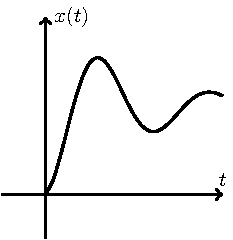
\includegraphics{segnale-continuo-1.pdf}%
    \label{fig:segnale-continuo-1}
\end{figure}

Campionando un segnale analogico si crea un segnale digitale, considerando prima alcune condizioni definite dal teorema del campionamento. Per campionare un segnale si estraggono
valori, o campioni, dal segnale analogico ogni intervallo $T$. Il segnale così ottenuto è un segnale discreto $x_n$ o $x[n]$, che presenta un valore ogni multiplo del tempo di campionamento $T$ 
scelto. 
\begin{equation*}
    x[n]:=\{x(n\cdot T)\,\forall n\in\mathbb{N}\}
\end{equation*}

\begin{figure}[H]%
    \centering
    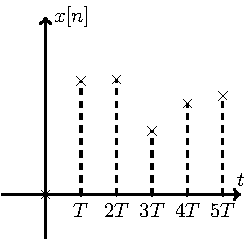
\includegraphics{segnale-discreto-1.pdf}%
    \label{fig:segnale-discreto-1}
\end{figure}

Questi valori vengono poi convertiti in digitale assegnando un certo numero di bit per rappresentare l'intervallo massimo di valori descritti dal segnale. Questo processo 
viene chiamato quantizzazione, si divide l'intervallo dei valori in piccoli intervalli ognuno con un univoco valore in bit, in modo da convertire tutti i valori in quell'intervallo in una sequenza di bit. Aumentando il numero di bit, quindi il numero di suddivisioni dell'intervallo di partenza, aumenta la precisione, ma aumenta anche il costo 
per processare lo stesso segnale. Dopo aver convertito tutti i valori in una sequenza di bit, questo segnale in bit viene tramesso, ed in seguito decodificato in analogico. 
Spesso i segnali vengono creati in digitale, per cui non è necessario campionare un segnale analogico. 


Campionando un segnale si perdono le informazioni contenute tra i campioni, ma è possibile applicare filtri e trasformazioni in digitale utili da giustificare la questa perdita 
di informazioni, per cui la maggior parte dei segnali vengono trasmessi in digitale. 




I segnali possono essere classificati in certi (deterministici) o aleatori (non deterministici). I segnali certi sono segnali di cui è noto tutto l'andamento, come file salvati su un supporto, per cui non è necessario 
trasmetterli. Mentre i segnali aleatori non sono noti a priori e vengono studiati dal punto di vista della statistica. 

In generale un sistema di trasmissione di segnali è formato da un trasmettitore che processa e codifica il segnale, un canale che lo trasmette, ed un ricevitore che lo decodifica:
\begin{figure}[H]%
    \centering
    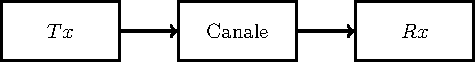
\includegraphics{canale-trasmissione.pdf}%
    \label{fig:canale-trasmissione}
\end{figure}

\clearpage

\section{Segnali Canonici}

\subsection{Segnali a Tempo Continuo}

Vengono definiti in questa sezione una serie di segnali canonici, e le operazioni attuabili su questo tipo di segnali:

\subsubsection{Seno Cardinale}

\begin{equation}
    x(t)=\sinc(t):=\displaystyle\frac{\sin(\pi t)}{\pi t}
\end{equation}
Questo segnale si attenua asintoticamente come $1/t$: 
\begin{equation*}
    \displaystyle-\frac{1}{t}\leq\sinc(t)\leq\frac{1}{t}
\end{equation*}
Viene incluso il fattore $\pi$ nell'argomento in modo che la funzione si annulli per ogni valore intero:
\begin{equation*}
    \sinc(t)=0\,\forall t\in\mathbb{Z}
\end{equation*}

\begin{figure}[H]%
    \centering
    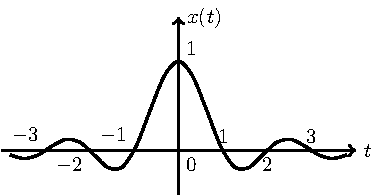
\includegraphics{seno-cardinale.pdf}%
\end{figure}

\subsubsection{Coseno}

\begin{equation}
    x(t)=\cos\left(\displaystyle\frac{2\pi t}{T}\right)
\end{equation}

Il parametro $T$ rappresenta il periodo della funzione, per cui il valore della funzione ad un certo valore $t$ corrisponde al valore in $t-T$. Invece del periodo si può 
usare la frequenza $f_0$, inverso del periodo. 

\begin{figure}[H]%
    \centering
    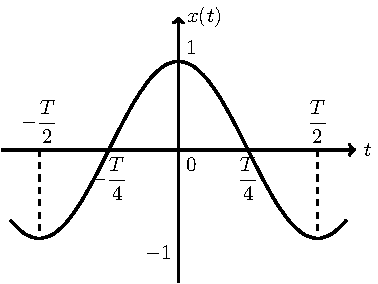
\includegraphics{coseno.pdf}%
\end{figure}

\subsubsection{Gradino Periodico o Onda Quadra}

\begin{figure}[H]%
    \centering
    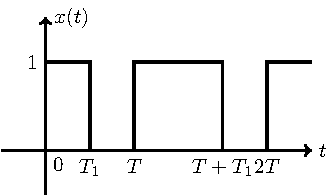
\includegraphics{onda-quadra.pdf}%
\end{figure}

\subsubsection{Esponenziale Complesso}

\begin{equation}
    x(t)=\displaystyle e^{i\frac{2\pi t}{T}}=\cos\left(\frac{2\pi t}{T}\right)+i\sin\left(\frac{2\pi t}{T}\right)
\end{equation}

Un segnale complesso può essere analizzato mediante la sua fase ed il suo modulo in funzione del tempo:
\begin{equation*}
    x(t)=|x(t)|e^{\phase{x(t)}}
\end{equation*}

Dato che la fase è periodica si può rappresentare come una serie di rampe.

\begin{figure}[H]%
    \centering
    \subfloat[\centering Modulo]{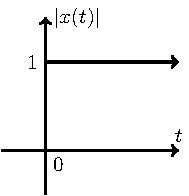
\includegraphics{esponenziale-complesso-modulo.pdf}}%
    \qquad
    \subfloat[\centering Fase]{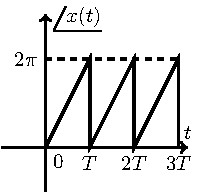
\includegraphics{esponenziale-complesso-fase.pdf}}%
\end{figure}

\subsubsection{Esponenziale}

\begin{equation}
    x(t)=e^{-\alpha t},\,\alpha\in\mathbb{R}
\end{equation}

\begin{figure}[H]%
    \centering
    \subfloat[\centering $\alpha<0$]{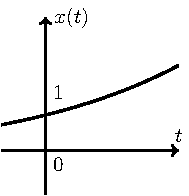
\includegraphics{esponenziale-1.pdf}}%
    \qquad
    \subfloat[\centering $\alpha >0$]{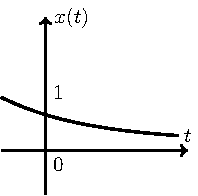
\includegraphics{esponenziale-2.pdf}}%
\end{figure}

\subsubsection{Finestra}

\begin{equation}
    x(t)=\rect\left(\displaystyle\frac{t}{T}\right):=\begin{cases}
        1 & \displaystyle-\frac{\strut T}{\strut 2}\leq t <\frac{\strut T}{\strut 2}\\
        0 & \displaystyle t<-\frac{\strut T}{\strut 2} \land t\geq\frac{\strut T}{\strut 2}
    \end{cases}
\end{equation}

$T$ viene chiamata base della finestra. Questo segnale presenta una discontinuità di salto per $t=\pm\displaystyle\frac{T}{2}$. La funzione finestra viene usata quando si 
vuole analizzare solo una parte di un segnale, poiché il restante sarà pari a $0$. La trasformata di questa funzione rappresenta un filtro in frequenza. 

\begin{figure}[H]%
    \centering
    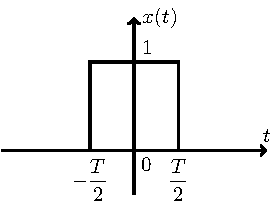
\includegraphics{finestra.pdf}%
\end{figure}

\subsubsection{Triangolo}

\begin{equation}
    x(t)=\mbox{tri}\left(\displaystyle\frac{t}{T}\right):=\begin{cases}
        1-|t| & -T\leq t < T\\
        0 & t<-T \land t\geq T
    \end{cases}
\end{equation}

\begin{figure}[H]%
    \centering
    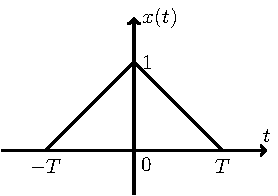
\includegraphics{triangolo.pdf}%
\end{figure}

\subsubsection{Gradino}

\begin{equation}
    x(t)=u(t):=\begin{cases}
        1 & t\geq0\\
        0 & t<0
    \end{cases}
\end{equation}

\begin{figure}[H]%
    \centering
    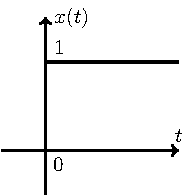
\includegraphics{gradino.pdf}%
\end{figure}

\subsubsection{Gaussiana}

\begin{equation}
    x(t)=e^{-\alpha t^2}\,\,\alpha\in\mathbb{R}^+
\end{equation}

La larghezza della campana centrale dipende dal fattore $\alpha$. Nello studio delle probabilità, si usa la sua forma normalizzata:
\begin{equation*}
    x(t)=\displaystyle\frac{e^{-\frac{t^2}{2\sigma^2}}}{\sqrt{2\pi}\sigma}
\end{equation*}
Il valore $\sigma$ rappresenta la deviazione standard, mentre il suo quadrato $\sigma^2$ descrive la varianza. 

\begin{figure}[H]%
    \centering
    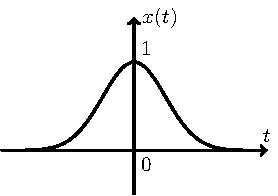
\includegraphics{gaussiana.pdf}%
\end{figure}

\subsubsection{Esponenziale Unilatero}

\begin{equation}
    x(t)=e^{-\alpha t}\cdot u(t)\,\,\alpha\in\mathbb{R}^+
\end{equation}

\begin{figure}[H]%
    \centering
    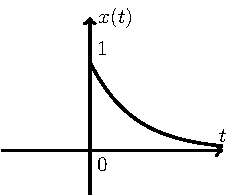
\includegraphics{esponenziale-unilatero.pdf}%
\end{figure}

\subsubsection{Costante}

\begin{equation}
    x(t)=a
\end{equation}
\begin{figure}[H]%
    \centering
    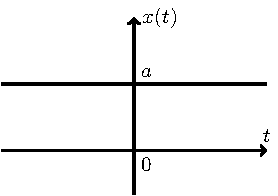
\includegraphics{costante.pdf}%
\end{figure}

\subsubsection{Segno}

\begin{equation}
    x(t)=\mbox{sign}(t):=\begin{cases}
        1&t>0\\
        -1&t<0
    \end{cases}
\end{equation}

\begin{figure}[H]%
    \centering
    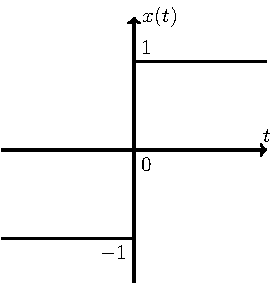
\includegraphics{segno.pdf}%
\end{figure}

\subsubsection{Operazioni sui Segnali}

Le operazioni sui segnali vengono computate istante per istante. L'operazione di somma produce un segnale $z(t)$, tale che ogni valore che assume equivale alla somma 
di altri due segnali $x(t)$ e $y(t)$ nello stesso istante:
\begin{equation*}
    z(t)=x(t)+y(t)
\end{equation*}

Analogamente si considera l'operazione prodotto, come un prodotto istante per istante tra i due segnali:
\begin{equation*}
    z(t)=x(t)\cdot y(t)
\end{equation*}

L'operazione di ribaltamento corrisponde ad una riflessione della funzione lungo l'asse delle ascisse di un segnale $x(t)$ tramite una sostituzione di variabile $t\to-t$:
\begin{equation*}
    z(t)=x(-t)
\end{equation*}
Quest'operazione non produce risultati per segnali pari, poiché presentano la proprietà $x(t)=x(-t)$. 
Tramite l'operazione di ribaltamento si può esprimere il segnale segno tramite la differenza di due gradini:
\begin{equation*}
    \mbox{sign}(t)=u(t)-u(-t)
\end{equation*}


L'operazione di traslazione, sposta un segnale $x(t)$ lungo l'asse delle ascisse di un fattore $\tau$:
\begin{equation*}
    z(t)=x(t-\tau)
\end{equation*}

L'operazione di cambio di scala corrisponde ad un rimpicciolimento o allargamento di un segnale $x(t)$ di un fattore $a\in\mathbb{R}$:
\begin{equation*}
    z(t)=x(at)
\end{equation*}

\subsubsection{Energia e Potenza}

L'energia e la potenza di un segnale rappresentano caratteristiche utili nella loro analisi e processamento. 

Viene definita energia $E_x$ di un segnale $x(t)$, come il limite per $\Delta t\to\infty$ dell'integrale del modulo quadro del segnale: 
\begin{equation}
    E_x:=\lim_{\Delta t\to\infty}\displaystyle\int_{-\frac{\Delta t}{2}}^{\frac{\Delta t}{2}}|x(t)|^2\df t=\int_{-\infty}^{\infty}|x(t)|^2\df t
\end{equation}
L'energia di un segnale è sempre strettamente positiva, poiché si considera tutta l'area sottesa dal quadrato del modulo del segnale, necessariamente positivo; mentre è nulla 
solo se lo è anche il segnale analizzato. Teoricamente non esiste un limite per l'energia contenuta in un segnale, ma sono fisicamente realizzabili solo segnali con energia 
finita. 

Se l'energia di un segnale è finita $E_x\neq\infty$ e diversa da zero $E_x\neq0$, il segnale $x(t)$ si chiama segnale di energia.


Viene definita la potenza $P_x$ di un segnale $x(t)$ in maniera simile alla sua energia:
\begin{equation}
    P_x:=\lim_{\Delta t\to\infty}\displaystyle\left(\frac{1}{\Delta t}\int_{-\frac{\Delta t}{2}}^{\frac{\Delta t}{2}}|x(t)|^2\df t\right)
\end{equation}
Anche la potenza di un segnale è strettamente positiva $P_x\geq0$, se la potenza assume valori diversi da zero e finiti, il segnale $x(t)$ si chiama segnale di potenza. 

Vengono così create due classi di segnali, di potenza e di energia. Per la definizione, queste due grandezze sono antisimmetriche poiché se un segnale è di potenza non può 
essere di energia, e viceversa: 
\begin{gather*}
    x\in E\implies x\notin P\\
    x\in P\implies x\notin E
\end{gather*}

Si determina l'energia di una gaussiana di ampiezza $A$:
\begin{gather*}
    E_x=\lim_{\Delta t\to\infty}\displaystyle\int_{-\frac{\Delta t}{2}}^{\frac{\Delta t}{2}}A^2e^{-2\alpha t^2}\df t=A^2\lim_{\Delta t\to\infty}\displaystyle\int_{-\frac{\Delta t}{2}}^{\frac{\Delta t}{2}}e^{-2\alpha t^2}\df t
\end{gather*}
Si considera il cambio di variabile $\tau=\sqrt{2\alpha}t$:
\begin{equation*}
    E_x=A^2\lim_{\Delta t\to\infty}\displaystyle\int_{-\frac{\Delta t}{2}}^{\frac{\Delta t}{2}}\frac{e^{-\tau^2}}{\sqrt{2\alpha}}\df\tau=\frac{A^2}{\sqrt{2\alpha}}\int_{-\infty}^{+\infty}e^{-\tau^2}\df\tau
\end{equation*}

L'integrale ottenuto è l'integrale di Gauss, risolubile applicando un cambio di coordinate polari al quadrato dell'integrale dato, il risultato dell'integrazione della 
gaussiana sull'intero asse dei reali $\mathbb{R}$ corrisponde alla radice di pi greco: 
\begin{equation*}
    \displaystyle\int_{\mathbb{R}}e^{-t^2}\df t=\sqrt\pi
\end{equation*}
Per cui l'energia di una gaussiana risulta essere:
\begin{equation}
    E_x=A^2\displaystyle\sqrt{\frac{\pi}{2\alpha}}
\end{equation}




Moltiplicando un segnale $x(t)$ per un gradino e calcolandone l'integrale su tutti i reali $\mathbb{R}$, equivale a calcolare l'integrale del segnale originario sui soli 
reali positivi $\mathbb{R}^+$, poiché il segnale assume valori nulli da $-\infty$ a $0$: 
\begin{equation*}
    \displaystyle\int_{\mathbb{R}}x(t)\cdot u(t)\df t=\int_{\mathbb{R}^+}x(t)\df t
\end{equation*}



Si determina l'energia e la potenza di un esponenziale complesso. Il segnale ha un modulo unitario $|x(t)|=1$, per cui la sua energia risultante è:
\begin{equation*}
    E_x=\lim_{\Delta t\to\infty}\displaystyle\int_{-\frac{\Delta t}{2}}^{\frac{\Delta t}{2}}\df t=\lim_{\Delta t\to\infty}\left(\frac{\Delta t}{2}+\frac{\Delta t}{2}\right)=\infty
\end{equation*}
Per cui l'esponenziale complesso non è un segnale di energia. La potenza risulta essere:
\begin{equation*}
    P_x=\lim_{\Delta t\to\infty}\displaystyle\left(\frac{1}{\Delta t}\int_{-\frac{\Delta t}{2}}^{\frac{\Delta t}{2}}\df t\right)=\lim_{\Delta t\to\infty}\left(\frac{1}{\Delta t}\cdot\Delta t\right)=1
\end{equation*}
L'esponenziale complesso è quindi un segnale di potenza. 



Si determina l'energia di un esponenziale unilatero:
\begin{equation*}
    E_x=\displaystyle\int_{-\infty}^{+\infty}\left[e^{-\alpha t}u(t)\right]^2\df t=\int_0^{+\infty}e^{-2\alpha t}\df t=-\frac{1}{2\alpha}\left(\cancelto{0}{e^{-\infty}}-\cancelto{1}{e^{0}}\right)=\frac{1}{2\alpha}
\end{equation*}
Per cui questo segnale non è né di energia né di potenza. 


I segnali periodici non possono essere di energia poiché l'integrale assume sempre valori non finiti, per cui un segnale periodico senza attenuazione non è fisicamente 
realizzabile. Possono essere solo di potenza, si determina la potenza di un segnale periodico:
\begin{equation*}
    P_x=\lim_{\Delta t\to\infty}\displaystyle\left(\frac{1}{\Delta t}\int_{-\frac{\Delta t}{2}}^{\frac{\Delta t}{2}}|x(t)|^2\df t\right)
\end{equation*}
In un segnale periodico si può esprimere l'intervallo di tempo $\Delta t$ come $n$ volte il periodo $T$:
\begin{equation*}
    P_x=\lim_{n\to\infty}\displaystyle\left(\frac{1}{n T}\int_{-\frac{nT}{2}}^{\frac{nT}{2}}|x(t)|^2\df t\right)
\end{equation*}
L'integrale di un segnale perfettamente periodico, ovvero senza smorzamenti, su $n$ periodi equivale ad $n$ volte l'integrale su un singolo periodo $T$:
\begin{equation*}
    P_x=\lim_{n\to\infty}\displaystyle\left(\frac{1}{n T}n\int_{-\frac{n}{2}}^{\frac{T}{2}}|x(t)|^2\df t\right)=\lim_{n\to\infty}\displaystyle\left(\frac{1}{T}\int_{-\frac{T}{2}}^{\frac{T}{2}}|x(t)|^2\df t\right)
\end{equation*} 
Questo integrale è indipendente dalla variabile $n$, per cui si può trascurare il limite, la potenza risulta quindi essere:
\begin{equation}
    P_x=\displaystyle\frac{1}{T}\int_{-\frac{T}{2}}^{\frac{T}{2}}|x(t)|^2\df t
\end{equation}
Quest'ultimo integrale può essere espresso in termini della frequenza naturale: $f_0=\frac{1}{T}$. 



Si determina la potenza del segnale coseno, di ampiezza $A$ e frequenza naturale $f_0$:
\begin{gather*}
    x(t)=A\cos\left(2\pi f_0t\right)\\
    P_x=\displaystyle A^2f_0\int_{-\frac{1}{2f_0}}^{\frac{1}{2f_0}}\cos^2(2\pi f_0 t)\df t
\end{gather*}
Per esprimere il quadrato del coseno, si considera la formula di bisezione del coseno:
\begin{gather*}
    \cos(2x)=2\cos^2(x)-1\\
    \cos^2(x)=\displaystyle\frac{\cos(2x)+1}{2}\\
    A^2\cos^2(2\pi f_0t)=\displaystyle\frac{A^2}{2}(\cos(4\pi f_0t)+1)
\end{gather*}
Si può esprimere inoltre mediante la notazione complessa delle funzioni trigonometriche:
\begin{gather*}
    A\cos(2\pi f_0t)=\displaystyle\frac{A}{2}(e^{2i\pi f_0t}+e^{-2i\pi f_0t})\\
    |x+y|^2\,\,x,y\in\mathbb{C}\\
    (x+y)\cdot(x+y)^*=(x+y)\cdot(x^*+y^*)\\
    xx^*+xy^*+yx^*+yy^*=|x|^2+|y|^2+xy^*+yx^*\\
    xy^*+yx^*=(a_x+ib_x)\cdot(a_y-ib_y)+(a_x-ib_x)\cdot(a_y+ib_y)=2(a_xa_y+b_xb_y)=2\Re\{x^*y\}\\
    |x|^2+|y|^2+2\Re\{|x|e^{-i\varphi_x}+|y|e^{i\varphi_y}\}\\
    |x|^2+|y|^2+2|x||y|\cos(|\varphi_y-\varphi_x|)\\
    \Bigg|\displaystyle\frac{A}{2}\left(e^{2i\pi f_0t}+e^{-2i\pi f_0t}\right)\Bigg|^2=\frac{A^2}{4}\left(1+1+2\Re\Bigl\{e^{2i\pi f_0t}\cdot\left(e^{-2i\pi f_0t}\right)^*\Bigr\}\right)\\
    A^2\cos^2(2\pi f_0t)=\displaystyle\frac{A^2}{2}(1+\cos(4\pi f_0t))
\end{gather*}
Considerando questa sostituzione, l'integrale diventa:
\begin{equation*}
    P_x=\displaystyle\frac{A^2f_0}{2}\int_{-\frac{1}{2f_0}}^{\frac{1}{2f_0}}(\cancelto{0}{\cos(4\pi f_0 t)}+1)\df t=\frac{A^2f_0}{2}\left(\frac{1}{2f_0}+\frac{1}{2f_0}\right)=\frac{A^2}{2}
\end{equation*}
L'integrale su un periodo del coseno è nullo, poiché è una funzione pari, per cui la componente $\cos(4\pi f_0 t)$ fornisce un contributo nullo. 

\clearpage

\subsection{Segnali a Tempo Discreto}

Poiché la maggior parte dei segnali vengono trasmessi o generati in tempo discreto, è necessario essere a conoscenza del comportamento dei segnali continui campionati a 
tempo discreto. 

\subsubsection{Gradino}

\begin{equation}
    x[n]=u[n]:=\begin{cases}
        1&n\geq0\\
        0&n<0
    \end{cases}
\end{equation}

\begin{figure}[H]%
    \centering
    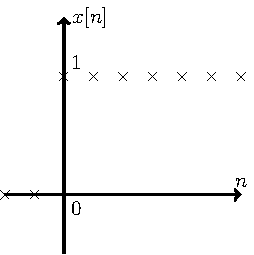
\includegraphics{gradino-discreto.pdf}%
\end{figure}

Non avendo un segnale finestra a tempo discreto, essa può essere descritta come la differenza di due gradini discreti. Una finestra di base $2l$ nel discreto si esprime come:
\begin{equation*}
    u[n+l]-u[n-(l+1)]
\end{equation*}

\begin{figure}[H]%
    \centering
    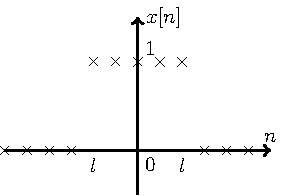
\includegraphics{finestra-discreto.pdf}%
\end{figure}

\subsubsection{Esponenziale Unilatero}

\begin{equation}
    x[n]=a^nu[n]
\end{equation}

\begin{figure}[H]%
    \centering
    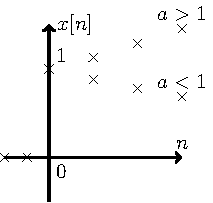
\includegraphics{esponenziale-unilatero-discreto.pdf}%
\end{figure}

\subsubsection{Coseno}

\begin{equation}
    x[n]=\cos(2\pi f_0n)
\end{equation}

Il segnale è periodico nel discreto, solo se la frequenza è un numero intero $f_0\in\mathbb{Z}$. 

\begin{figure}[H]%
    \centering
    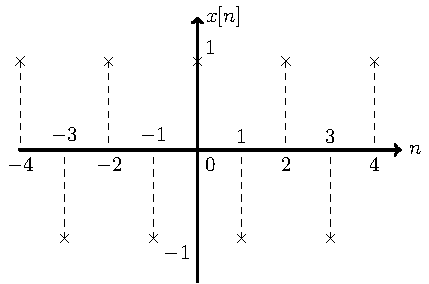
\includegraphics{coseno-discreto.pdf}%
\end{figure}

\subsubsection{Impulso Matematico Tempo Discreto}

L'impulso matematico o delta di Dirac, nel discreto assume solo un valore di $1$ per $n=0$. 
\begin{equation}
    \delta[n]:=\begin{cases}
        1&n=0\\
        0&n\neq0
    \end{cases}
\end{equation}

Questo segnale presenta varie proprietà utili:


L'area della delta è unitaria, poiché presenta un unico campione per $n=0$ di valore $1$:
\begin{equation*}
    \displaystyle\sum_{n=-\infty}^{+\infty}\delta[n]=1
\end{equation*}



Il prodotto di un qualsiasi segnale $x[n]$ per la delta equivale al valore del segnale in $0$ per la delta. Poiché l'unico valore della delta diverso da zero si trova in $n=0$ 
e vale $1$, per cui estrae dal segnale $x$ il campione in posizione $n=0$. Questo campione viene moltiplicato per la delta, poiché non è un segnale continuo, ma si presenta 
solo in quell'istante. Questa caratteristica viene chiamata proprietà di campionamento 
della delta di Dirac:
\begin{equation*}
    x[n]\cdot\delta[n]=x[0]\cdot\delta[n]
\end{equation*}
Questo campione può essere estratto ad un arbitraria posizione $m$:
\begin{equation*}
    x[n]\cdot\delta[n-m]=x[m]\cdot\delta[n-m]
\end{equation*}


L'area del prodotto di un qualsiasi segnale $x[n]$ per la delta risulta nel valore del segnale in $0$, ciò si dimostra tramite la proprietà di campionamento della delta:
\begin{equation*}
    \displaystyle\sum_{n=-\infty}^{+\infty} x[n]\cdot\delta[n]=\sum_{n=-\infty}^{+\infty} x[0]\cdot\delta[n]=x[0]\cancelto{1}{\sum_{n=-\infty}^{+\infty}\delta[n]}=x[0]
\end{equation*}


Invertendo la proprietà di campionamento, ovvero partendo da tutti i campioni di un segnale $x[n]$ e sommandoli tra di loro, è possibile ottenere il segnale originario: 
\begin{equation*}
    \cdots+x[-N]\delta[n+N]+\cdots+x[0]\delta[n]+\cdots+x[N]\delta[n-N]+\cdots=\displaystyle\sum_{k=-\infty}^{+\infty} x[k]\delta[n-k]=x[n]
\end{equation*}


La convoluzione di un qualsiasi segnale $x[n]$ per la delta risulta nel segnale $x$ stesso:
\begin{equation*}
    x[n]*\delta[n]=\displaystyle\sum_{k=-\infty}^{+\infty}x[k]\delta[n-k]=\sum_{k=-\infty}^{+\infty}x[n]\delta[n-k]=x[n]\cancelto{1}{\sum_{k=-\infty}^{+\infty}\delta[n-k]}
\end{equation*}


La delta può essere rappresentata come la differenza tra due gradini, considerando un unico campione in posizione $m$:
\begin{equation*}
    \delta[n-m]=u[n-m]-u[n-(m+1)]
\end{equation*}


Analogamente un gradino può essere espresso come una somma di impulsi traslati ognuno di un diverso fattore. Questa relazione viene espressa in forma canonica come:
\begin{equation*}
    u[n-m]=\displaystyle\sum_{n=-\infty}^{-m}\delta[n+1]
\end{equation*}

\subsubsection{Energia e Potenza}

L'energia di un segnale tempo discreto si calcola come:
\begin{equation*}
    E_x:=\displaystyle\lim_{N\to\infty}\sum_{n=-N}^N|x[n]|^2
\end{equation*}
La potenza di un segnale tempo discreto è definita come:
\begin{equation*}
    P_x:=\displaystyle\lim_{N\to\infty}\left(\frac{1}{2N+1}\sum_{n=-N}^N|x[n]|^2\right)
\end{equation*}
La potenza per segnali periodici tempo discreti si ottiene mediante:
\begin{equation*}
    P_x:=\displaystyle\frac{1}{M}\sum_{n=0}^{M-1}|x[n]|^2
\end{equation*}
Dove $M$ è il periodo del segnale.

\clearpage

\section{Convoluzione e Correlazione}

Prima di analizzare queste due importanti operazioni tra segnali tempo continuo e discreto, bisogna fornire una definizione adeguata per l'impulso matematico tempo 
continuo, segnale utile nello studio, e nel calcolo di queste operazioni.  

\subsection{Impulso Matematico Tempo Continuo}

Per definire l'impulso o delta di Dirac nel tempo continuo, si parte da un segnale finestra con una base $\Delta t$ e ampiezza inverso della base:
\begin{equation*}
    x(t)=\displaystyle\frac{1}{\Delta t}\rect\left(\frac{t}{\Delta t}\right)
\end{equation*}

\begin{figure}[H]%
    \centering
    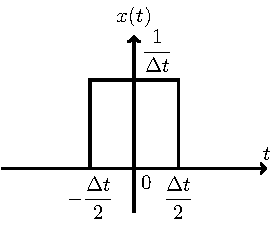
\includegraphics{impulso-finestra.pdf}%
\end{figure}

Al diminuire di $\Delta t$, la base si restringe, mentre l'ampiezza del segnale aumenta, ma complessivamente l'area del segnale rimane costante:
\begin{equation*}
    \displaystyle\int_{-\infty}^{+\infty}x(t)\df t=\frac{1}{\Delta t}\int_{-\frac{\Delta t}{2}}^{\frac{\Delta t}{2}}\df t=\frac{1}{\Delta t}\left(\frac{\Delta t}{2}+\frac{\Delta t}{2}\right)=1
\end{equation*}

Viene definito l'impulso o delta di Dirac come il limite di questa finestra per $\Delta t$ che tende ad un valore nullo:
\begin{equation}
    \delta(t):=\lim_{\Delta t\to0}\displaystyle\frac{1}{\Delta t}\rect\left(\frac{t}{\Delta t}\right)
\end{equation}

Viene rappresentata graficamente come una freccia di altezza unitaria, poiché non è una funzione ma un funzionale, ma questa differenza non verrà trattata nei seguenti 
studi.  
\begin{figure}[H]%
    \centering
    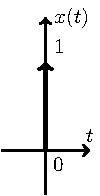
\includegraphics{impulso.pdf}%
\end{figure}

Possiede delle proprietà analoghe alla delta nel tempo discreto:



L'integrale sui reali della delta è unitario in base alla sua definizione:
\begin{equation*}
    \displaystyle\int_{-\infty}^{+\infty}\delta(t)\df t=1
\end{equation*}



Il prodotto di un qualsiasi segnale per la delta equivale al valore del segnale in $0$ moltiplicato per l'impulso, poiché per tutti gli altri valori nel tempo questo prodotto 
è nullo. Proprietà analoga a quella del campionamento, per il continuo:
\begin{equation*}
    x(t)\cdot\delta(t)=x(0)\cdot\delta(t)
\end{equation*}
Questa proprietà può essere estesa considerando un impulso traslato di un fattore $\tau$:
\begin{equation*}
    x(t)\cdot\delta(t-\tau)=x(\tau)\cdot\delta(t-\tau)
\end{equation*}



Segue da quest'ultima che l'integrale del prodotto di un segnale qualunque $x(t)$ per l'impulso equivale al valore del segnale $x$ in $0$:
\begin{equation*}
    \displaystyle\int_{-\infty}^{+\infty}x(t)\cdot\delta(t)\df t=\int_{-\infty}^{+\infty}x(0)\cdot\delta(t)\df t=x(0)\cancelto{1}{\int_{-\infty}^{+\infty}\delta(t)\df t}=x(0)
\end{equation*}



La convoluzione di un qualsiasi segnale $x(t)$ con l'impulso risulta nel segnale originario $x(t)$, per l'inverso della proprietà precedente: 
\begin{equation*}
    x(t)*\delta(t)=\displaystyle\int_{-\infty}^{+\infty}x(\tau)\cdot\delta(t-\tau)\df\tau=x(t)\cancelto{1}{\int_{-\infty}^{+\infty}\delta(t-\tau)\df\tau}=x(t)
\end{equation*}



Poiché il segnale finestra può essere espresso come la differenza tra due gradini, allora anche la definizione dell'impulso può essere espressa come tale:
\begin{equation*}
    \delta(t):=\lim_{\Delta t\to\infty}\frac{1}{\Delta t}\left(u\left(t+\frac{\Delta t}{2}\right)-u\left(t-\frac{\Delta t}{2}\right)\right)
\end{equation*}



L'impulso corrisponde alla derivata rispetto al tempo del gradino. Analogamente il gradino corrisponde alla funzione integrale dell'impulso:
\begin{gather*}
    \delta(t)=\displaystyle\frac{\df u(t)}{\df t}\\
    u(t)=\displaystyle\int_{-\infty}^t\delta(\tau)\df\tau
\end{gather*}



L'impulso è una funzione pari:
\begin{equation*}
    \delta(t)=\delta(-t)
\end{equation*}



L'impulso scalato di un fattore $a$ corrisponde al rapporto tra l'impulso non scalato ed il modulo del fattore $a$, se negativo. Questa proprietà di scala si dimostra 
considerando la definizione dell'impulso: 
\begin{gather*}
    \delta(at)=\displaystyle\lim_{\Delta t\to0}\frac{1}{\Delta t}\rect\left(\frac{at}{\Delta t}\right)\\
    \Delta\tau=\displaystyle\frac{\Delta t}{a}\\
    \displaystyle\lim_{\Delta\tau\to0}\frac{1}{a\Delta\tau}\rect\left(\frac{t}{\Delta\tau}\right)=\frac{1}{a}\lim_{\Delta\tau\to0}\frac{1}{\Delta\tau}\rect\left(\frac{t}{\Delta\tau}\right)\\
    \delta(at)=\displaystyle\frac{\delta(t)}{a}
\end{gather*}



L'impulso è un segnale né di energia né di potenza. I funzionali, come l'impulso, vengono descritti in base agli effetti che provocano sulle funzioni

\subsection{Convoluzione}

La convoluzione rappresenta un'operazione tra due segnali, generandone uno nuovo. L'operazione si indica con il simbolo $*$:
\begin{equation*}
    x(t)*y(t)=z(t)
\end{equation*}

La convoluzione tra due segnali tempo continui produce sempre un segnale continuo: 
\begin{equation}
    z(t)=x(t)*y(t):=\displaystyle\int_{-\infty}^{+\infty}x(\tau)\cdot y(t-\tau)\df\tau
\end{equation}

Il segnale convoluzione è una funzione nella stessa variabile dei segnali convoluti, questa variabile di uscita compare all'interno dell'integrale. Il segnale convoluzione 
rappresenta l'area sottesa dal prodotto tra il segnale $x$ ed il segnale $y$, ribaltato e traslato di un fattore $t$, per ogni istante di tempo $t$. La convoluzione 
è un'operazione commutativa, per cui è arbitraria la scelta di quale dei due segnali debba traslare. 

Si rappresenta il segnale $x$ originario rispetto alla variabile $\tau$, al di sotto si grafica il segnale $y$ ribaltato e traslato di un fattore $t$, per individuare gli 
intervalli dove il prodotto tra i due segnali è nullo. La maggior parte dei segnali reali si attenuano nel tempo, per cui avranno un valore diverso da zero solo per un 
intervallo finito di valori, ed in questi intervalli la convoluzione restituisce un valore non nullo. Anche i segnali puramente matematici spesso presentano valori finiti 
non nulli solo per certi intervalli di tempo. Si considerano tutti i possibili casi di sovrapposizione, quindi di prodotto non nullo, tra i due segnali, per ottenere 
il segnale convoluzione in forma analitica. Da notare che la convoluzione è un segnale continuo per cui non possono essere presenti discontinuità nella sua espressione 
in forma analitica. 

\subsubsection{Proprietà}

La convoluzione è un'operazione commutativa:
\begin{equation*}
    x(t)*y(t)=\displaystyle\int_{-\infty}^{+\infty}x(\tau)y(t-\tau)\df\tau\to{T=t-\tau}\to \int_{-\infty}^{+\infty}y(T)x(t-T)\df T=y(t)*x(t)
\end{equation*}
Vale la proprietà distributiva:
\begin{gather*}
    (x_1(t)+x_2(t))*y(t)=\displaystyle\int_{-\infty}^{+\infty}(x_1(\tau)+x_2(\tau))y(t-\tau)\df\tau\\
    \int_{-\infty}^{+\infty}x_1(\tau)y(t-\tau)\df\tau+\int_{-\infty}^{+\infty}x_2(\tau)y(t-\tau)\df\tau=x_1(t)*y(t)+x_2(t)*y(t)
\end{gather*}

Se uno dei due segnali convoluti, o entrambi, sono traslati allora il segnale convoluzione risultante è traslato della traslazione complessiva dei due segnali originali:
\begin{gather*}
    x(t-t_{x0})*y(t-t_{y0})=\displaystyle\int_{-\infty}^{+\infty}x(\tau-t_{x0})y[t-(\tau+t_{y0})]\df\tau\\
    {T=\tau-t_{x0}}\\\
    \int_{-\infty}^{+\infty}x(T)y[(t-t_{x0}-t_{y0})+T]\df T=z(t-t_{x0}-t_{y0})
\end{gather*}

\subsubsection{Convoluzione Tempo Discreto}

\begin{equation*}
    x[n]*y[n]:=\displaystyle\sum_{k=-\infty}^{+\infty}x[k]y[n-k]
\end{equation*}

Nel discreto, quando si applica la convoluzione, il numero di campioni totali della convoluzione è uguale alla somma dei campioni dei due segnali meno uno. Per le convoluzioni 
a tempo continuo si usa la continuità, per quelle a tempo discreto il numero dei campioni, per identificare se sono convoluzioni valide. Per le convoluzioni a tempo discreto valgono le proprietà 
commutativa e distributiva. I singoli campioni di un segnale nel discreto possono essere rappresentati come una costante che moltiplica un impulso traslato di un certo fattore:
\begin{equation*}
    x[n]=\displaystyle\sum_{k=1}^Nx_k\delta[n-k]
\end{equation*}
Ciò è possibile per ogni segnale discreto, per cui la convoluzione di due segnali discreti si può esprimere come:
\begin{equation*}
    x[n]*y[n]=\displaystyle\sum_{k=-\infty}^{+\infty}x[k]y[n-k]=\sum_{k=-\infty}^{+\infty}\left[\sum_{i=1}^Nx_i\delta[k-i]\sum_{j=1}^Ny_j\delta[n-k-j]\right]
\end{equation*}
Una convoluzione quindi rappresenta una media tra una serie di campioni, può essere estesa a segnali multidimensionali come delle immagini, dove la convoluzione viene 
usata negli algoritmi di compressione dell'immagini per diminuire il costo della trasmissione del segnale, diminuendo l'informazione necessaria. 

\subsection{Correlazione}
\label{sec:correlazione}
La correlazione è un'operazione simile alla convoluzione, calcolabile come una convoluzione. Le convoluzioni vengono usate per modellare l'effetto del passaggio di un segnale 
attraverso un sistema, ciò corrisponde al processamento di un segnale. Alcuni di questi sistemi corrispondono nel dominio della frequenza in filtri. 


Una correlazione si applica quando due segnali sono simili tra loro, viene definita come un segnale continuo nel dominio del tempo:
\begin{equation}
    R_{xy}(t)=x(t)\otimes y(t)=\int_{-\infty}^{+\infty}x(t+\tau)y^*(\tau)\df\tau
\end{equation}
Viene definito $R_{xy}$ il fattore di correlazione tra i due segnali $x$ e $y$. La correlazione al contrario della convoluzione non commuta:
\begin{gather*}
    \displaystyle R_{xy}(t)=\int_{-\infty}^{+\infty}x(t+\tau)y^*(\tau)\df\tau\\
    T=t+\tau\\
    \displaystyle\int_{-\infty}^{+\infty}x(T)y^*(-t+T)\df T=\left[\int_{-\infty}^{+\infty}x^*(T)y(-t+T)\df T\right]^*=R_{yx}^*(-t)
\end{gather*}
Il fattore di convoluzione $R_{xy}(t)$ tra due segnali $x$ e $y$ corrisponde al complesso coniugato del fattore di convoluzione ribaltato dei segnali $y$ e $x$ $R_{yx}^*(-t)$, 
quindi la correlazione è un'operazione anticommutativa. La correlazione tra due segnali $x$ e $y$ equivale alla convoluzione dei segnali $y^*$ e $x$
\begin{gather*}
    x(t)\otimes y(t)=\displaystyle\int_{-\infty}^{+\infty}x(t+\tau)y^*(\tau)\df\tau\\
    x(t)*y^*(-t)=\displaystyle\int_{-\infty}^{+\infty}x(\tau)y^*(-(t-\tau))\df\tau\\
    T=\tau-t\\
    -\int_{+\infty}^{-\infty}x(t+T)y^*(T)\df T=\int_{-\infty}^{+\infty}x(t+T)y^*(T)\df T=R_{xy}(t)\\
    x(t)\otimes y(t)=x(t)*y^*(-t)
\end{gather*}
Quando si analizza la correlazione tra due segnali $x$ e $y$, uno dei quali pari $y(t)=y(-t)$ e reale $y\in\mathbb{R}$, la correlazione tra di loro è uguale alla convoluzione 
tra di loro:
\begin{equation*}
    x(t)\otimes y(t)=x(t)*y^*(-t)=x(t)*y(-t)=x(t)*y(t)
\end{equation*}

L'autocorrelazione di un segnale $x$ nell'istante di tempo $t=0$, corrisponde all'energia del segnale:
\begin{equation*}
    R_{xx}(0)=\displaystyle\int_{-\infty}^{+\infty}x(\tau)x^*(\tau)\df\tau=\int_{-\infty}^{+\infty}|x(\tau)|^2\df\tau=E_x
\end{equation*}

\subsection{Sistema Ingresso-Uscita}

Un sistema di ingresso-uscita applica determinate trasformazioni al segnale $x$ in entrata, per ottenere un altro segnale $y$ in uscita, questo segnale è un funzionale 
del segnale di ingresso $y(t)=\mathcal{F}\{x(t)\}$. Questa trasformazione si basa su dei parametri interni $\sum$ al sistema per cui passa l'ingresso. 
\begin{figure}[H]%
    \centering
    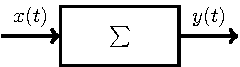
\includegraphics{sistema-io.pdf}%
\end{figure}

Un sistema ingresso-uscita si definisce lineare, se ad una combinazione lineare degli ingressi, corrisponde una combinazione lineare delle uscite:
\begin{equation*}
    x(t)=a_1(t)x_1(t)+\cdots+a_n(t)x_n(t)\to y(t)=b_1(t)y_1(t)+\cdots+b_n(t)y_n(t)
\end{equation*}

Un amplificatore rappresenta un sistema lineare, poiché moltiplica di un fattore $A$ un segnale in entrata:
\begin{gather*}
    x_1(t)\to y_1(t)=Ax_1(t)\\
    x_2(t)\to y_2(t)=Ax_2(t)\\
    ax_1(t)+bx_2(t)\to ay_1(t)+by_2(t)=A(ax_1(t)+bx_2(t))
\end{gather*} 
\begin{figure}[H]%
    \centering
    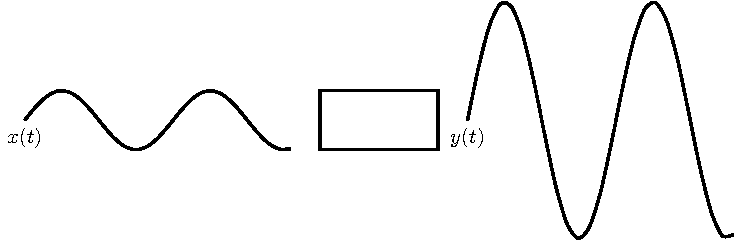
\includegraphics{amplificatore.pdf}%
\end{figure}
Un sistema lineare non distorce gli ingressi. Un sistema che restituisce il segnale originario sommato per una costante $A$ non è lineare:
\begin{gather*}
    x(t)\to y(t)=x(t)+A\\
    x_1(t)+x_2(t)\to y(t)=x_1(t)+x_2(t)+A\neq y_1(t)+y_2(t)
\end{gather*}


Un sistema tempo invariante o permanente, non dipende da quando viene inserito il segnale in entrata:
\begin{gather*}
    x(t)\to y(t)\\
    x(t-\tau)\to y(t-\tau)
\end{gather*}
La linearità e la permanenza sono due proprietà indipendenti tra di loro. Un sistema può essere lineare e non permanente e viceversa, oppure nessuno delle due. 
L'operazione di modulazione di un segnale, il prodotto tra l'entrata ed una funzione sinusoidale, è un sistema lineare e non permanente:
\begin{gather*}
    x(t)\to y(t)=x(t)\cos\displaystyle\left(\frac{2\pi t}{T}\right)\\
    x(t-\tau)\to y(t-\tau)=x(t-\tau)\displaystyle\cos\left(\frac{2\pi t}{T}\right)\neq x(t-\tau)\cos\left(\frac{2\pi (t-\tau)}{T}\right)
\end{gather*}
Per cui dipende dall'istante di tempo quando viene inserito il segnale. 


Un sistema può presentare un'altra proprietà chiamata causalità, che presenta un senso fisico. Un sistema si definisce causale se per ogni uscita all'istante $t_0$, dipende 
da valori entrati al massimo fino al tempo $t_0$: 
\begin{equation*}
    y(t_0)\propto x(t),\,\,t\leq t_0
\end{equation*}
L'uscita non può dipendere da entrate future, se il sistema è causale.
Data un'uscita $y$ dipendente dall'entrata $x$ traslata di un fattore $\tau$ $y(t)=x(t+\tau)$, se questo fattore di traslazione $\tau$ è negativo, l'uscita dipende da entrate ritardate 
per cui dipende da entrate passate, mentre se il fattore $\tau$ è positivo l'uscita dipende da entrate anticipate, quindi per un certo istante $t$ l'uscita dipende da entrate 
future. 


La linearità e la permanenza sono due proprietà fondamentali per cui un sistema si identifica come filtro, o SLI, Sistema Lineare Invariante. L'uscita di un filtro dipende 
solo da una funzione $h(t)$, chiamata risposta impulsiva, e si ottiene mediante la convoluzione tra l'entrata e quest'ultima:
\begin{equation*}
    x(t)\to y(t)=x(t)*h(t)
\end{equation*}
Si chiama risposta impulsiva, poiché se è presente un impulso in entrata, l'uscita è la funzione $h(t)$ stessa, per la proprietà della convoluzione di un impulso:
\begin{equation*}
    \delta(t)\to y(t)=\delta(t)*h(t)=h(t)
\end{equation*}

Per dimostrare l'uscita di un filtro, si considera il segnale $x$ come la somma integrale di impulsi moltiplicati per il valore della funzione in $x(\tau)$, ovvero la sua 
convoluzione:
\begin{gather*}
    x(t)=x(t)*\delta(t)=\displaystyle\int_{-\infty}^{+\infty}x(\tau)\delta(t-\tau)\df\tau=\int_{-\infty}^{+\infty}\df x(t)
\end{gather*}
Poiché il filtro è lineare si può considerare l'uscita $y$ come la somma integrale di tutte le uscite $\df y$ per ogni entrata $\df x=x(\tau)\delta(t-\tau)\df\tau$. Poiché il fattore 
$x(\tau)$ non dipende dal tempo si considera una costante, per cui l'uscita $\df y$ uguale al prodotto tra la costante $x(\tau)$ per la convoluzione tra l'impulso e la 
risposta impulsiva:
\begin{gather*}
    \df x(t)=x(\tau)\delta(t-\tau)\df\tau\\
    \df y(t)=x(\tau)(\delta(t-\tau)*h(t))\df\tau=x(\tau)h(t-\tau)\df\tau
\end{gather*}
L'uscita totale si ottiene integrando su tutti i reali l'uscita infinitesima $\df y(t)$:
\begin{equation*}
    y(t)=\displaystyle\int_{-\infty}^{+\infty}\df y(t)=\int_{-\infty}^{+\infty}x(\tau)h(t-\tau)\df\tau=x(t)*h(t)
\end{equation*}
Per cui l'uscita di un filtro corrisponde alla convoluzione tra l'entrata e la sua risposta impulsiva. 

Per determinare la risoluzione di uno schermo, dispositivo che opera come un filtro, si inserisce in entrata un impulso bidimensionale, rappresentato come un singolo punto 
su una superficie. L'uscita di questa entrata risulta in una macchia formata da vari pixel; più questa macchia è piccola maggiore è la risoluzione del dato schermo.  



Nel tempo discreto un sistema può essere caratterizzato dalle stesse proprietà. 
Linearità:
\begin{gather*}
    x_1[n]\to y_1[n]\\
    x_2[n]\to y_2[n]\\
    a_1x_1[n]+a_2x_2[n]\to a_1y_1[n]+a_2y_2[n]
\end{gather*}
Tempo invarianza:
\begin{gather*}
    x[n+N]\to y[n+N]
\end{gather*}
Causalità:
\begin{equation*}
    y[n_0]\propto x[n],\,\, n\leq n_0
\end{equation*}
Si può esprimere formalmente questa condizione di causalità considerando un filtro con una risposta impulsiva $h[n]$:
\begin{equation*}
    y[n]=\displaystyle\sum_{k=-\infty}^{+\infty}x[k]h[n-k]
\end{equation*} 
Se questo filtro fosse causale allora la variabile $k$ non potrebbe superare il valore $n$, poiché ciò implicherebbe che l'uscita dipenda da entrate future:
\begin{equation*}
    y[n]=\displaystyle\sum_{k=-\infty}^nx[k]h[n-k]
\end{equation*}
Inoltre la risposta impulsiva deve essere nulla se il valore di $k$ è maggiore di $n$:
\begin{equation*}
    h[n-k]=0,\,\, k>n\to{n-k=N}\to h[N],\,\, N<0
\end{equation*} 
Si può attuare lo stesso ragionamento per la causalità a tempo continuo. Un filtro è causale solo se:
\begin{gather*}
    y(t)=\displaystyle\int_{-\infty}^{+\infty}x(\tau)h(t-\tau)\df\tau\to \int_{-\infty}^{t}x(\tau)h(t-\tau)\df\tau\\
    h(t-\tau)=0,\,\, \tau>t\to{t-\tau=T}\to h(T)=0,\,\, T<0
\end{gather*}
Per cui si definisce un filtro di uscita $y$ causale se e solo se:
\begin{equation*}
    y(t):\mbox{ causale}\iff \begin{cases}
        h[n]=0& n<0\\
        h(t)=0& t<0
    \end{cases}
\end{equation*}


Un filtro operante su tempo discreto viene definito, come nel continuo, da un'unica funzione risposta impulsiva $h[n]$:
\begin{equation*}
    \delta[n]*h[n]=h[n]
\end{equation*}
Si esprime per la proprietà di campionamento dell'impulso, un qualsiasi segnale $x$ come:
\begin{equation*}
    x[n]=\displaystyle\sum_{k=-\infty}^{+\infty}x[k]\delta[n-k]
\end{equation*}
Poiché il filtro è un sistema lineare, si possono considera le singole entrate della sommatoria e poi sommare le loro uscite corrispondenti per ottenere l'uscita complessiva. 
Si considera l'uscita per un qualsiasi $k$, pari alla convoluzione tra l'impulso $\delta[n-k]$ e la risposta impulsiva $h[n]$, si considera il parametro $x[k]$ costante poiché 
non dipende dalla variabile $n$:
\begin{equation*}
    y_k[n]=x[k](\delta[n-k]*h[n])=x[k]h[n-k]
\end{equation*}
La somma su tutti gli interi di questo valore $y_k$ corrisponde all'uscita totale $y$ del sistema per l'entrata $x$:
\begin{equation*}
    y[n]=\displaystyle\sum_{k=-\infty}^{+\infty}y_k[n]=\sum_{k=-\infty}^{+\infty}x[k]h[n-k]=x[n]*h[n]
\end{equation*}
Questa uscita $y$ corrisponde alla convoluzione tra l'entrata $x$ e la risposta impulsiva $h$. 


Data la struttura del sistema è possibile individuare l'uscita in forma analitica rispetto ad una generica entrata. Dopo aver determinato la risposta impulsiva inserendo 
al posto di una generica entrata $x$ l'impulso $\delta$, è possibile sostituire l'intero modello strutturale del sistema con un singolo blocco funzionale, un'oggetto che 
applica all'entrata la convoluzione per i parametri contenuti, contenente la risposta impulsiva.  
Si considera un generico schema di un circuito sommatore, un tipo di sistema controllore a feedforward:
\begin{figure}[H]%
    \centering
    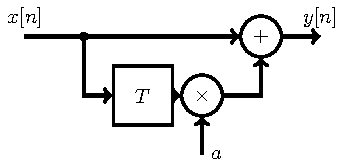
\includegraphics{circuito-1.pdf}%
\end{figure}
Per ottenere l'uscita si somma il segnale originario allo stesso segnale ritardato di un campione e moltiplicato per un fattore $a$:
\begin{gather*}
    y[n]=x[n]+ax[n-1]\\
    h[n]=\delta[n]+a\delta[n-1]
\end{gather*}
\begin{figure}[H]%
    \centering
    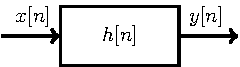
\includegraphics{sistema-io-discreto.pdf}%
\end{figure}

\subsection{Convoluzione tra Due Gaussiane}

Date due gaussiane definite dai parametri $\alpha_1$ e $\alpha_2$, con $\alpha_1,\alpha_2\in\mathbb{R}^+$, si vuole determinare la convoluzione tra questi due segnali:
\begin{gather*}
    z(t)=e^{-\alpha_1t^2}*e^{-\alpha_2t^2}=\displaystyle\int_{-\infty}^{+\infty}e^{-\alpha_1\tau^2}e^{-\alpha_2(t-\tau)^2}\df\tau=\int_{-\infty}^{+\infty}e^{-\alpha_1\tau^2}e^{-\alpha_2(t^2-2t\tau+\tau^2)}\df\tau\\
    \displaystyle e^{-\alpha_2 t^2}\int_{-\infty}^{+\infty}e^{-(\alpha_1+\alpha_2)\tau^2}e^{2\alpha_2t\tau^2}\df\tau=e^{-\alpha_2 t^2}\int_{-\infty}^{+\infty}e^{-(\alpha_1+\alpha_2)\left[\tau^2-2\alpha_2\frac{t\tau}{\alpha_1+\alpha_2}\right]}\df\tau
\end{gather*}

Si somma e si sottrae il fattore $\displaystyle\left(\frac{\alpha_2t}{\alpha_1+\alpha_2}\right)^2$ nell'esponenziale all'interno dell'integrale:
\begin{gather*}
    \displaystyle e^{-\alpha_2 t^2}\int_{-\infty}^{+\infty}e^{-(\alpha_1+\alpha_2)\left[\tau^2-2\alpha_2\frac{t\tau}{\alpha_1+\alpha_2}+\left(\frac{\alpha_2t}{\alpha_1+\alpha_2}\right)^2-\left(\frac{\alpha_2t}{\alpha_1+\alpha_2}\right)^2\right]}\df\tau\\
    \displaystyle e^{-\alpha_2 t^2}\int_{-\infty}^{+\infty}e^{-(\alpha_1+\alpha_2)\left[\left(\tau-\frac{\alpha_2t}{\alpha_1+\alpha_2}\right)^2-\left(\frac{\alpha_2t}{\alpha_1+\alpha_2}\right)^2\right]}\df\tau\\
    \displaystyle e^{-\left(\alpha_2-\frac{\alpha_2^2}{\alpha_1+\alpha_2}\right)t^2}\int_{-\infty}^{+\infty}e^{-(\alpha_1+\alpha_2)\left[\tau-\frac{\alpha_2t}{\alpha_1+\alpha_2}\right]^2}\df\tau
\end{gather*}
Si applica la sostituzione $T=\displaystyle\sqrt{\alpha_1+\alpha_2}\left(\tau+\frac{\alpha_2t}{\alpha_1+\alpha_2}\right)$:
\begin{equation*}
    \displaystyle e^{-\left(\frac{\alpha_1\alpha_2}{\alpha_1+\alpha_2}\right)t^2}\int_{-\infty}^{+\infty}\frac{e^{-T^2}}{\sqrt{\alpha_1+\alpha_2}}\df T=\frac{e^{-\left(\frac{\alpha_1\alpha_2}{\alpha_1+\alpha_2}\right)t^2}}{\sqrt{\alpha_1+\alpha_2}}\int_{-\infty}^{+\infty}{e^{-T^2}}\df T
\end{equation*}
Il fattore integrale corrisponde all'integrale di Gauss, precedentemente discusso, che risulta su tutti i reali in un area di $\sqrt\pi$:
\begin{equation*}
    e^{-\alpha_1t^2}*e^{-\alpha_2t^2}=\displaystyle\sqrt{\frac{\pi}{\alpha_1+\alpha_2}}e^{-\frac{\alpha_1\alpha_2}{\alpha_1+\alpha_2}t^2}
\end{equation*}
Esprimendo le due gaussiane in forma normalizzata, risulta che la varianza della convoluzione equivale alla somma delle varianze delle due gaussiane $\sigma=\sigma_1+\sigma_2$:
\begin{equation}
    \displaystyle\frac{1}{\sqrt{2\pi}\sigma_1}e^{-\frac{t^2}{2\sigma_1}}*\frac{1}{\sqrt{2\pi}\sigma_2}e^{-\frac{t^2}{2\sigma_2}}=\frac{1}{\sqrt{2\pi(\sigma_1^2+\sigma_2^2)}}e^{-\frac{t^2}{2(\sigma_1^2+\sigma_2^2)}}
\end{equation}

\subsection{Convoluzione a Media Mobile}
Calcolare la convoluzione tra una finestra ed un segnale periodico $y$, 
per semplificare i calcoli si considera il segnale coseno, ma le proprietà ottenute da quest'operazione valgono per ogni funzione periodica, non attenuata nel tempo. 

\begin{equation*}
    z(t)=\rect\displaystyle\left(\frac{t}{T_1}\right)*\cos\left(\frac{2\pi t}{T_2}\right)=\int_{-\infty}^{+\infty}\cos\left(\frac{2\pi \tau}{T_2}\right)\rect\displaystyle\left(\frac{t-\tau}{T_1}\right)\df\tau
\end{equation*}
La funzione è periodica per cui non è necessario valutare quando la convoluzione è nulla. Il prodotto tra i due segnali è non nullo per valori di $\tau$ compresi tra 
$\displaystyle\frac{T_1}{2}-t$ e $-\displaystyle\frac{T_1}{2}-t$:
\begin{gather*}
    z(t)=\displaystyle\int_{-\frac{T_1}{2}-t}^{\frac{T_1}{2}-t}\cos\left(\frac{2\pi\tau}{T_2}\right)\df\tau=\frac{T_2}{2\pi}\sin\left(\frac{2\pi\tau}{T_2}\right)\Bigg|_{-\frac{T_1}{2}-t}^{\frac{T_1}{2}-t}\\
    \displaystyle\frac{T_2}{2\pi}\left[\sin\left(\frac{2\pi(t+\frac{T_1}{2})}{T_2}\right)-\sin\left(\frac{2\pi(t-\frac{T_1}{2})}{T_2}\right)\right]
\end{gather*}
Per la seconda formula di prostaferesi si ottiene:
\begin{gather*}
    z(t)=\displaystyle\frac{T_2}{2\pi}\cos\left(\frac{2\pi}{T_2}t\right)\sin\left(\frac{2\pi}{T_2}\frac{T_1}{2}\right)=\left[\frac{T_2}{2\pi}\sin\left(\pi\frac{T_1}{T_2}\right)\right]\cos\left(\frac{2\pi t}{T_2}\right)
\end{gather*}
Se il periodo del coseno è uguale alla base della finestra, il seno è sempre nullo, quindi anche la convoluzione è nulla per ogni valore di $t$. I fattori invarianti nel 
tempo si possono esprimere come una costante $A$, ampiezza del segnale ottenuto:
\begin{equation*}
    \rect\left(\displaystyle\frac{t}{T_1}\right)*\cos\left(\frac{2\pi t}{T_2}\right)=A\cos\left(\frac{2\pi t}{T_2}\right)
\end{equation*}  
Il risultato della convoluzione è il segnale periodico originario moltiplicato per un fattore costante, che dipende dal periodo $T_2$ e dalla base del segnale finestra $T_1$. 
Il segnale di convoluzione quindi oscilla come la funzione periodica di partenza. In generale il risultato della convoluzione di una finestra con una funzione periodica è un fattore 
$A$ moltiplicato per il segnale originario:
\begin{equation}
    \rect\left(\frac{t}{T_1}\right)*y(t)=A(T_1,T_2)y(t)
\end{equation}

Questa proprietà si indica come un'operazione a media mobile, che amplifica o riduce l'ampiezza di un segnale periodico, oppure lo rende nullo. 

\clearpage

\section{Serie di Fourier}

Dati due segnali di frequenza doppia come il La$4$ a $\approx 440Hz$ ed il La$5$ a $\approx 880Hz$, non si nota la differenza poiché sono esattamente una il doppio dell'altra. 
In generale segnali musicali affinché suonino bene devono avere frequenze tra di loro o multipli oppure relati da frazioni semplici, non possono essere scelte arbitrariamente. 
Queste frequenze sono associate a varie note, inserendo una serie di queste note è possibile scrivere un segnale musicale. Viene attuato un processo analogo tramite la serie di 
Fourier. Questo tipo di analisi venne introdotta da Fourier nella sua teoria analitica del calore, dove oltre all'omonima serie e trasformata, introdusse molti concetti 
matematici importanti. 



La serie di Fourier è uno strumento per esprimere solo i segnali periodici, 
se il segnale non è periodico si usa la trasformata di Fourier, se rispetta le condizioni di Dirichlet, ma per i nostri fini si considerano sempre verificate. 
I segnali si esprimono rispetto alle sue armoniche. Dato un segnale $x(t)$ di periodo $T$, può essere rappresentato come una serie, ovvero una sommatoria, di alcuni 
coefficienti di Fourier per un fattore esponenziale, chiamato armonica, di frequenza multiplo della frequenza del segnale originario:
\begin{equation}
    x(t)=\displaystyle\sum_{k=-\infty}^{+\infty}c_ke^{i\frac{2\pi  k t}{T}}
\end{equation}
Il fattore $c_k$ indica se una data frequenza è presente nel segnale analizzato. Le armoniche sono note a priori, dal punto di vista fisico non esistono armoniche di frequenze 
negative, ma in ambito matematico sono necessarie per esprimere il segnale. Considerando la rappresentazione di Eulero si può esprimere la serie di Fourier come:
\begin{equation}
    x(t)=\displaystyle\sum_{k=-\infty}^{+\infty}c_k\left[\cos\left(\frac{2\pi k t}{T}\right)+i\sin\left(\frac{2\pi k t}{T}\right)\right]
\end{equation}
Poiché le armoniche sono le stesse, l'unica differenza tra varie rappresentazioni di Fourier è il valore dei coefficienti $c_k$ assegnati. Lo spazio dei segnali periodici, 
aventi lo stesso periodo $T$, può essere scritto come uno spazio vettoriale dotato di prodotto scalare, dove ogni segnale è espresso come un vettore. Questo spazio può essere 
espresso data una base ortonormale.

\subsection{Spazio Vettoriale}

Si considera uno spazio euclideo $\mathbb{R}^3$ descritto da tre vettori ortonormali $\hat x=(1,0,0)$, $\hat y=(0,1,0)$ e $\hat z=(0,0,1)$, chiamati base canonica dello spazio vettoriale. 
Dei vettori di uno spazio vettoriale si dicono base, se sono ortonormali tra di loro, quindi il prodotto scalare tra di loro è nullo ovvero sono linearmente indipendenti, 
mentre si dicono basi canoniche se il quadrato di un vettore, il prodotto scalare per sé stesso, equivale ad uno. 
Il prodotto scalare è un'operazione binaria interna ad uno spazio vettoriale $V$ che restituisce uno scalare:
\begin{equation*}
    \langle \cdot \; , \; \cdot \rangle : V \times V  \rightarrow \mathbb{R}
\end{equation*}
Si definisce come il prodotto matriciale tra il primo vettore per la trasposta del secondo:
\begin{equation*}
    \langle\vec v,\,\vec w\rangle=\vec v\cdot \vec w^T=\begin{pmatrix}
        v_x &v_y&v_z
    \end{pmatrix}\cdot\begin{pmatrix}
        w_x\\ w_y \\ w_z
    \end{pmatrix}
\end{equation*} 
Per ottenere una certa componente di un generico vettore $\vec{v}$ si considera il prodotto tra quel vettore e la base della componente desiderata:
\begin{equation*}
    \langle\vec v,\,\hat x\rangle=\vec v\cdot \hat x^T=\begin{pmatrix}
        v_x &v_y&v_z
    \end{pmatrix}\cdot\begin{pmatrix}
        1\\ 0 \\0
    \end{pmatrix}=v_x
\end{equation*} 



Il segnale periodico $x(t)$ può essere scritto come una somma di coefficienti moltiplicati per una base ortonormale dello spazio vettoriale dei segnali periodici di periodo 
$T$. In questo spazio sono presenti infiniti vettori ortonormali tra di loro, a differenza dello spazio euclideo $\mathbb{R}^3$, dove sono presenti tre vettori base. Questo 
spazio è quindi uno spazio euclideo di dimensione numerabile, ma infinita, poiché le basi ortonormali corrispondono alle infinite armoniche di periodo $T$. 
Il prodotto scalare tra due segnali $x$ e $y$ viene definito come:
\begin{equation*}
    \langle x(t),\,y(t)\rangle=x(t)\cdot y(t)=\displaystyle\int_{-\infty}^{+\infty}x(t)\cdot y^*(t)\df t
\end{equation*}
Il prodotto scalare tra due segnali periodici viene definito come:
\begin{equation*}
    \langle x(t),\,y(t)\rangle=x(t)\cdot y(t)=\displaystyle\frac{1}{T}\int_{-\frac{T}{2}}^{\frac{T}{2}}x(t)\cdot y^*(t)\df t
\end{equation*}
Per cui per ottenere i coefficienti di Fourier $c_k$ rispetto ad una determinata armonica $k$ di un segnale $x$ si considera il prodotto scalare tra quel segnale per l'
armonica $k$:
\begin{equation}
    c_k=\langle x(t),\,e^{i\frac{2\pi  k t}{T}}\rangle=\displaystyle\frac{1}{T}\int_{-\frac{T}{2}}^{\frac{T}{2}}x(t)\cdot e^{-i\frac{2\pi  k t}{T}}\df t
\end{equation} 

Il prodotto tra due basi è nullo, tranne nel caso dove sono la stessa base, in quel caso il risultato è $1$. Per dimostrare che le armoniche rappresentano una base dello 
spazio vettoriale si considera il prodotto scalare tra un'armonica $k$ ed una $l$:
\begin{gather*}
    \langle e^{i\frac{2\pi kt}{T}},e^{i\frac{2\pi lt}{T}}\rangle=\displaystyle\frac{1}{T}\int_{-\frac{T}{2}}^{\frac{T}{2}}e^{i\frac{2\pi kt}{T}}e^{-i\frac{2\pi lt}{T}}\df t=
    \frac{1}{T}\left[e^{i\frac{2\pi(k-l)t}{T}}\frac{T}{2i\pi (k-l)}\right]^{\frac{T}{2}}_{-\frac{T}{2}}\\
    \displaystyle\frac{e^{i\pi(l-k)}-e^{-i\pi(l-k)}}{2i}\frac{1}{\pi (k-l)}=\frac{\sin(\pi(k-l))}{\pi (k-l)}
\end{gather*} 
Questa funzione risulta essere una sinc, e per definizione è un segnale che si annulla per ogni valore intero, e poiché $k$ e $l$ sono due interi la loro differenza lo è 
poiché l'insieme degli interi è chiuso rispetto alla somma: $k-l\in\mathbb{Z}$. Quindi il prodotto scalare tra due armoniche $k$ e $l$, non triviale: $k\neq l$, è di valore 
nullo:
\begin{equation*}
    \forall k\neq l\in\mathbb{Z}\implies \langle e^{i\frac{2\pi kt}{T}},e^{i\frac{2\pi lt}{T}}\rangle=0
\end{equation*}
\'{E} stato dimostrato che le armoniche sono una base dello spazio vettoriale dei segnali periodici di periodo $T$. 
Per $k=0$ l'armonica corrispondente è un segnale costante. In generale un'armonica di ordine $k$ si può esprimere mediante la rappresentazione di Eulero:
\begin{equation*}
    \displaystyle e^{i\frac{2\pi kt}{T}}=\cos\left(\frac{2\pi kt}{T}\right)+i\sin\left(\frac{2\pi kt}{T}\right)
\end{equation*}
Per cui la parte reale di un'armonica oscilla come un segnale coseno di frequenza dell'armonica. 

\subsection{Serie Notevoli}

Si considera un segnale costante $x(t)=A$. Per determinare i coefficienti della sua serie di Fourier si considera il prodotto scalare tra il segnale ed una generica armonica $k$: 
\begin{gather*}
    c_k=\langle x(t),e^{i\frac{2\pi kt}{T}}\rangle=\displaystyle\frac{1}{T}\int_{-\frac{T}{2}}^{\frac{T}{2}}Ae^{-i\frac{2\pi kt}{T}}\df t=\left[A\frac{e^{-i\frac{2\pi kt}{T}}}{-2i\pi k}\right]_{-\frac{T}{2}}^{\frac{T}{2}}\\
    \displaystyle\frac{A(e^{-i\pi k}-e^{i\pi k})}{-2i\pi k}=A\frac{-\sin(\pi k)}{-\pi k}=A\,\sinc[k]
\end{gather*}
L'unico valore per cui il seno cardinale discreto in funzione di $k$ assume un valore non nullo è per $k=0$:
\begin{equation*}
    c_0=A\,\cancelto{1}{\sinc[0]}\to x(t)=c_0e^{\cancelto{0}{i\frac{2\pi kt}{T}}}
\end{equation*}

Si considera un coseno di periodo $T$: $x(t)=A\cos\left(\frac{2\pi t}{T}\right)$. Si vuole determinare la sua espansione di Fourier, per cui si considera il suo prodotto 
scalare con una generica armonica $k$. Si esprime il coseno tramite le formule di Eulero, in questo modo assume la stessa forma di una differenze di due armoniche: 
\begin{gather*}
    c_k=\displaystyle\frac{1}{T}\int_{-\frac{T}{2}}^{\frac{T}{2}}A\cos\left(\frac{2\pi t}{T}\right)e^{-i\frac{2\pi kt}{T}}\df t=
    \frac{A}{2T}\left(\int_{-\frac{T}{2}}^{\frac{T}{2}}e^{i\frac{2\pi t}{T}}e^{-i\frac{2\pi kt}{T}}\df t+\int_{-\frac{T}{2}}^{\frac{T}{2}}e^{-i\frac{2\pi t}{T}}e^{-i\frac{2\pi kt}{T}}\df t\right)
\end{gather*}
Il prodotto scalare tra due armoniche è stato precedentemente individuato come un seno cardinale:
\begin{equation*}
    \displaystyle c_k=\frac{A\,\sinc[1-k]+A\,\sinc[-(1+k)]}{2}
\end{equation*}
Il seno cardinale nel discreto assume gli stessi valori dell'impulso discreto. 
Quindi il coefficiente è nullo per ogni $k\neq1\lor-1$, gli unici coefficienti non nulli della sua serie di Fourier sono $c_{-1}$ e $c_1$:
\begin{gather*}
    \displaystyle c_1=c_{-1}=\frac{A}{2}\\
    \displaystyle x(t)=c_{-1}e^{-i\frac{2\pi t}{T}}+c_1e^{i\frac{2\pi t}{T}}
\end{gather*}


Si applica un processo analogo per determinare l'espansione di Fourier di un segnale sinusoidale $x(t)=\sin\left(\frac{2\pi t}{T}\right)$:
\begin{gather*}
    c_k=\displaystyle\frac{1}{T}\int_{-\frac{T}{2}}^{\frac{T}{2}}A\sin\left(\frac{2\pi t}{T}\right)e^{-i\frac{2\pi kt}{T}}\df t=
    \frac{A}{2iT}\left(\int_{-\frac{T}{2}}^{\frac{T}{2}}e^{i\frac{2\pi t}{T}}e^{-i\frac{2\pi kt}{T}}\df t-\int_{-\frac{T}{2}}^{\frac{T}{2}}e^{-i\frac{2\pi t}{T}}e^{-i\frac{2\pi kt}{T}}\df t\right)\\
    \displaystyle c_k=\frac{A\,\sinc[1-k]-A\,\sinc[-(1+k)]}{2i}\\
    c_1=-c_{-1}=\frac{A}{2i}\\
    x(t)=c_{-1}e^{-i\frac{2\pi t}{T}}+c_1e^{i\frac{2\pi t}{T}}
\end{gather*}
Altrimenti è possibile calcolare i coefficienti tramite confronto diretto dalla rappresentazione di Eulero delle funzioni trigonometriche, in questo modo si individuano le due 
armoniche che producono il segnale sinusoidale, di ordine $1$ e $-1$. 


Si considera ora un segnale $x(t)=A\cos^2\left(\frac{2\pi t}{T}\right)$. Per le formula di duplicazione del coseno si può riscrivere come:
\begin{equation*}
    A\cos^2\left(\frac{2\pi t}{T}\right)=\frac{A}{2}\left(\cos\left(\frac{4\pi t}{T}\right)+1\right)
\end{equation*}
Si calcola il valore di un coefficiente generico $k$:
\begin{gather*}
    c_k=\displaystyle\frac{1}{T}\int_{-\frac{T}{2}}^{\frac{T}{2}}A\cos^2\left(\frac{2\pi t}{T}\right)e^{-i\frac{2\pi kt}{T}}\df t=
    \frac{A}{2T}\int_{-\frac{T}{2}}^{\frac{T}{2}}\left(\cos\left(\frac{4\pi t}{T}\right)+1\right)e^{-i\frac{2\pi kt}{T}}\df t\\
    \displaystyle\frac{A}{2T}\left(\int_{-\frac{T}{2}}^{\frac{T}{2}}e^{i\frac{4\pi t}{T}}e^{-i\frac{2\pi kt}{T}}\df t+\int_{-\frac{T}{2}}^{\frac{T}{2}}e^{-i\frac{4\pi t}{T}}e^{-i\frac{2\pi kt}{T}}\df t+\int_{-\frac{T}{2}}^{\frac{T}{2}}e^{-i\frac{2\pi kt}{T}}\df t\right)\\
    \displaystyle\frac{A}{2}\left(2\,\sinc[2-k]-2\,\sinc[-(2+k)]+\sinc[k]\right)
\end{gather*}
I coefficienti non si annullano per valori di $k$ pari a $\pm2$ e $0$:
\begin{equation*}
    x(t)=c_{-2}e^{-i\frac{4\pi t}{T}}+c_0+c_2e^{i\frac{4\pi t}{T}}
\end{equation*}


Si considera un segnale onda quadra di periodo $T$ e di base $\tau$: 
\begin{equation*}
    x(t)=\displaystyle\sum_{n=-\infty}^{+\infty}\rect\left(\frac{t-nT}{\tau}\right)
\end{equation*}
Si determina il valore di un coefficiente generico $k$:
\begin{gather*}
    c_k=\displaystyle\frac{1}{T}\int_{-\frac{T}{2}}^{\frac{T}{2}}\sum_{n=-\infty}^{+\infty}\rect\left(\frac{t-nT}{\tau}\right)e^{-i\frac{2\pi k t}{T}}\df t
\end{gather*}
Nell'intervallo $[-T/2,T/2]$ cade una sola finestra di base $\tau$, per $n=0$, per cui si può riscrivere come:
\begin{gather*}
    c_k=\displaystyle\frac{1}{T}\int_{-\frac{T}{2}}^{\frac{T}{2}}\rect\left(\frac{t}{\tau}\right)e^{-i\frac{2\pi k t}{T}}\df t=\frac{1}{T}\int_{-\frac{\tau}{2}}^{\frac{\tau}{2}}e^{-i\frac{2\pi k t}{T}}=
    \left[\frac{e^{-i\frac{2\pi kt}{T}}}{-2i\pi k}\right]_{-\frac{\tau}{2}}^{\frac{\tau}{2}}\\
    \displaystyle\frac{e^{-i\pi k\frac{\tau}{T}}-e^{i\pi k\frac{\tau}{T}}}{-2i}\frac{1}{\pi k}=\frac{\tau}{T}\frac{\sin\left(\frac{\pi k \tau}{T}\right)}{\frac{\pi k \tau}{T}}=\frac{\tau}{T}\sinc\left(\frac{k \tau}{T}\right)
\end{gather*}

Il seno cardinale non è discreto, poiché l'argomento non necessariamente assume valore intero. 
\begin{equation*}
    x(t)=\displaystyle\sum_{n=-\infty}^{+\infty}\rect\left(\frac{t-nT}{\tau}\right)=\sum_{k=-\infty}^{+\infty}\frac{\tau}{T}\sinc\left(\frac{k \tau}{T}\right)e^{i\frac{2\pi kt}{T}}
\end{equation*}
All'aumentare di $k$ e quindi della frequenza delle armoniche, il valore dei coefficienti diminuisce, quindi diminuiscono anche i contributi delle armoniche a frequenza 
maggiore per la ricostruzione del segnale originale. I coefficienti rappresentano il peso di quanto le armoniche contribuiscono al segnale originario. La precisione 
aumenta sempre di meno per ogni nuova armonica aggiunta, fino a ricostruire completamente il segnale originale se $k$ tende asintoticamente ad infinito. Da notare che se 
$T=2\tau$, per $k$ pari i coefficienti della serie di Fourier dell'onda quadra che ha periodo esattamente il doppio della base sono nulli. In generale se $T=n\tau$, dove 
$n\in\mathbb{N}$, i contributi delle armoniche con frequenza multiplo di $n/T$ sono nulli, ovvero i coefficienti con $k$ multiplo di $n$ sono nulli:
\begin{gather*}
    c_k=\frac{1}{n}\sinc\left(\frac{k}{n}\right)=0\;\forall k=\alpha\cdot n,\;\alpha\in\mathbb{Z}
\end{gather*}
In generale se $T/\tau\notin\mathbb{Z}$ e $\tau/T\notin\mathbb{Z}$, i coefficienti dell'espansione di Fourier non sono mai nulli, poiché non comprendono mai zeri triviali 
della funzione seno cardinale. 



Per cui in generale il contenuto informativo del segnale è descritto interamente dai coefficienti della serie di Fourier $c_k$. 
A volte viene richiesto di individuare il periodo del segnale trattato per poi individuare i coefficienti della sua serie di Fourier.

\subsection{Proprietà}

\subsubsection{Linearità}

Poiché segnali $x(t)$ e $y(t)$, periodici di periodo $T$, possono essere espressi come espansione di Fourier rispetto alle stesse armoniche, la loro combinazione lineare 
può essere espressa come una combinazione lineare dei coefficienti delle due serie di Fourier:
\begin{gather*}
    x(t)=\displaystyle\sum_{k=-\infty}^{+\infty}c_ke^{i\frac{2\pi  k t}{T}}\\    
    y(t)=\displaystyle\sum_{k=-\infty}^{+\infty}d_ke^{i\frac{2\pi  k t}{T}}\\
    ax(t)+by(t)=\displaystyle\sum_{k=-\infty}^{+\infty}(ac_k+bd_k)e^{i\frac{2\pi  k t}{T}}\\
    \displaystyle\frac{1}{T}\int_{-\frac{T}{2}}^{\frac{T}{2}}(ax(t)+by(t))\df t=\frac{a}{T}\int_{-\frac{T}{2}}^{\frac{T}{2}}x(t)e^{-i\frac{2\pi  k t}{T}}\df t
    +\frac{b}{T}\int_{-\frac{T}{2}}^{\frac{T}{2}}y(t)e^{-i\frac{2\pi  k t}{T}}\df t=ac_k+bd_k
\end{gather*}

Data un'onda quadra $z(t)$ che assume valori di $1$ e $-1$ periodicamente, con periodo $T$, può essere espressa come una differenza tra due onde quadre $x(t)$ e $y(t)$ in 
opposizione di fase che assumono valori di $1$ e $0$ con periodo $T$. Una delle quali ha una base di lunghezza $\tau$, mentre l'altra lunghezza di $T-\tau$ e traslata di un 
semi-periodo $T/2$:
\begin{equation*}
    z(t)=\displaystyle\sum_{k=-\infty}^{+\infty}\left[\rect\left(\frac{t-kT}{\tau}\right)-\rect\left(\frac{t-nT-\frac{T}{2}}{T-\tau}\right)\right]
\end{equation*}

\begin{figure}[H]%
    \centering
    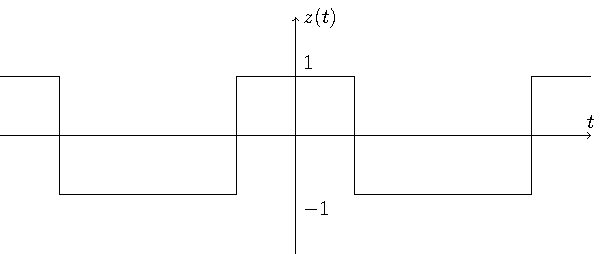
\includegraphics{onda-quadra-2.pdf}%
\end{figure}

Si calcolano ora i coefficienti dell'espansione di Fourier:
\begin{gather*}
    a_k=\displaystyle\frac{1}{T}\int_{-\frac{T}{2}}^{\frac{T}{2}}\left[\rect\left(\frac{t-kT}{\tau}\right)-\rect\left(\frac{t-kT-\frac{T}{2}}{T-\tau}\right)\right]\df t\\
    \displaystyle\frac{1}{T}\int_{-\frac{\tau}{2}}^{\frac{\tau}{2}}\rect\left(\frac{t-kT}{\tau}\right)\df t-\frac{1}{T}\int_{-\frac{T-\tau}{2}}^{\frac{T-\tau}{2}}\rect\left(\frac{t-kT-\frac{T}{2}}{T-\tau}\right)\df t\\
    \displaystyle\frac{e^{-i\pi k\frac{\tau}{T}}-e^{i\pi k\frac{\tau}{T}}}{-2i}\frac{1}{\pi k}\frac{\tau}{T}-\frac{e^{-i2\pi k\frac{T-\tau/2}{T}}-e^{i2\pi k\frac{T-\tau/2}{T}}}{-2i}\frac{1}{\pi k}\frac{\tau}{T}
\end{gather*}
Per $k=0$ si ottiene una forma indeterminata, per cui bisogna risolvere l'integrale considerando il valor medio assunto dal segnale nell'intervallo $\left[-T/2,T/2\right]$. 
\begin{gather*}
    \displaystyle\frac{\tau}{T}\sinc\left(\frac{k\tau}{T}\right)-\frac{e^{i\pi k\frac{\tau}{T}}-e^{-i\pi k\frac{\tau}{T}}}{-2i}\frac{1}{\pi k}\\
    c_k=\displaystyle\frac{2\tau}{T}\sinc\left(\frac{k\tau}{T}\right)
\end{gather*}


Generalmente si differenziano i casi dove l'esponenziale assume valore unitario, per $k=0$, dai casi dove è presente un'armonica generica. 

Il segnale originale può essere espresso come un'onda quadra doppia, di stesso periodo $T$ e base $\tau$, e traslata verso il basso:
\begin{equation*}
    z(t)=\displaystyle\sum_{k=-\infty}^{+\infty}\left[2\,\rect\left(\frac{t-kT}{\tau}\right)\right]-1=2x(t)-1
\end{equation*}
In questo modo si effettuano meno calcoli per determinare i coefficienti di Fourier, usufruendo della proprietà di linearità bisogna tenere conto che il fattore costante $-1$, 
assume un valore non nullo solo per $k=0$. Si considerano i coefficienti del segnale $x$ come $c_k$, mentre del segnale costante $d_k$, per cui in questo caso i coefficienti 
del segnale $z$ si esprimono come: 
\begin{equation*}
    a_k=\begin{cases}
        2c_k+d_k &k=0\\
        2c_k&k\neq0
    \end{cases}=\begin{cases}
        \displaystyle\frac{\strut 2\tau}{\strut T}-1&k=0\\
        \displaystyle\frac{\strut 2\tau}{\strut T}\sinc\left(\frac{ k\tau}{ T}\right)&k\neq0
    \end{cases}
\end{equation*}

\subsubsection{Traslazione nel Tempo}

Si considera un segnale ritardato nel tempo di un fattore $t_0$: $x(t-t_0)$, dati i coefficienti del segnale non traslato $c_k$. Per confronto diretto si ottiene:
\begin{gather*}
    x(t)=\displaystyle\sum_{k=-\infty}^{+\infty}c_ke^{i\frac{2\pi kt}{T}}\\
    x(t-t_0)=\displaystyle\sum_{k=-\infty}^{+\infty}c_ke^{i\frac{2\pi k(t-t_0)}{T}}=\sum_{k=-\infty}^{+\infty}\left(c_ke^{-i\frac{2\pi kt_0}{T}}\right)e^{i\frac{2\pi kt}{T}}\\
    x(t-t_0)=\displaystyle\sum_{k=-\infty}^{+\infty}d_ke^{i\frac{2\pi kt}{T}}
\end{gather*}
Per cui tutti i coefficienti equivalgono ai coefficienti non traslati $c_k$ moltiplicati per un fattore esponenziale, che dipende dalla traslazione $t_0$:
\begin{equation*}
    \displaystyle d_k=c_ke^{-i\frac{2\pi kt_0}{T}}
\end{equation*}

Altrimenti si possono determinare i coefficienti tramite la definizione, attuando una sostituzione $t-t_0\to\tau$:
\begin{gather*}
    d_k=\displaystyle\frac{1}{T}\int_{-\frac{T}{2}}^{\frac{T}{2}}x(t-t_0)e^{-i\frac{2\pi kt}{T}}\df T\to\int_{-\frac{T}{2}-t_0}^{\frac{T}{2}-t_0}x(\tau)e^{-i\frac{2\pi kt_0}{T}}e^{-i\frac{2\pi k\tau}{T}}\df\tau\\
    d_k=\displaystyle\frac{1}{T}e^{-i\frac{2\pi kt_0}{T}}\int_{-\frac{T}{2}-t_0}^{\frac{T}{2}-t_0}x(\tau)e^{-i\frac{2\pi k\tau}{T}}\df\tau=e^{-i\frac{2\pi kt_0}{T}}c_k
\end{gather*}
Dove $c_k$ sono i coefficienti del segnale non traslato. 


%grafico(?)
% EX:
Si considera un'onda quadra di periodo $T$ traslata di un fattore $\tau$, corrispondente alla lunghezza della sua base. Dati i coefficienti di un onda quadra non traslata 
$c_k$ si possono esprimere direttamente i coefficienti del segnale traslato $d_k$:
\begin{equation*}
    d_k=\displaystyle\frac{\tau}{T}\sinc\left(\frac{k\tau}{T}\right)e^{-i\frac{2\pi k\tau}{T}}
\end{equation*}

In caso il periodo sia esattamente il doppio della base $T=2\tau$:
\begin{equation*}
    d_k=\displaystyle\frac{1}{2}\sinc\left(\frac{k}{2}\right)e^{-i\pi k}=\frac{1}{2}\frac{e^{i\frac{\pi k}{2}}-e^{-i\frac{\pi k}{2}}}{i\pi k}e^{-i\pi k}=
    \frac{e^{-i\frac{\pi k}{2}}-e^{-i\frac{3\pi k}{2}}}{2i\pi k}
\end{equation*}
Per cui i coefficienti dell'onda quadra di armoniche di ordine pari risultano nulli. 

\subsubsection{Traslazione in Frequenza}

Si considera un segnale $x$ moltiplicato per un'armonica di ordine $n$:
\begin{equation*}
    y(t)=x(t)\cdot e^{i\frac{2\pi nt}{T}}=\displaystyle\sum_{k=-\infty}^{+\infty}c_ke^{i\frac{2\pi kt}{T}}e^{i\frac{2\pi nt}{T}}=\sum_{k=-\infty}^{+\infty}c_ke^{i\frac{2\pi (k+n)t}{T}}
\end{equation*}
Si considera la sostituzione $l=n+k$:
\begin{equation*}
    y(t)=\displaystyle\sum_{l=-\infty}^{+\infty}c_{l-n}e^{i\frac{2\pi lt}{T}}
\end{equation*}

Per cui i coefficienti dell'espansione di Fourier di $y$, corrispondo agli stessi coefficienti del segnale originario $x$, ma ad un generico coefficiente $c_k$ viene 
associata l'armonica di ordine $k+n$.   
Tramite la definizione integrale dei coefficienti di Fourier, si arriva allo stesso risultato:
\begin{gather*}
    \langle y(t),\;e^{i\frac{2\pi kt}{T}}\rangle=\displaystyle\frac{1}{T}\int_{-\frac{T}{2}}^{\frac{T}{2}}\left(x(t)\cdot e^{i\frac{2\pi nt}{T}}\right)e^{-i\frac{2\pi kt}{T}}\df t=\frac{1}{T}\int_{-\frac{T}{2}}^{\frac{T}{2}}x(t)\left(e^{i\frac{2\pi nt}{T}}e^{-i\frac{2\pi kt}{T}}\right)\df t\\
    \displaystyle\frac{1}{T}\int_{-\frac{T}{2}}^{\frac{T}{2}}x(t)e^{i\frac{2\pi (n-k)t}{T}}\df t=d_k=c_{k-n}
\end{gather*}
Si ottiene lo stesso risultato, i coefficienti associati alle armoniche vengono traslati di un fattore $n$, fattore del ritardo in frequenza del segnale.  

\subsubsection{Teorema della Modulazione}

Quando un segnale viene moltiplicato per un coseno ad una determinata frequenza si indica quest'operazione come modulazione. 
\begin{gather*}
    y(t)=x(t)\cos\displaystyle\left(\frac{2\pi t}{T}\right)=x(t)\left[\frac{e^{i\frac{2\pi t}{T}}+e^{-i\frac{2\pi t}{T}}}{2}\right]=\sum_{k=-\infty}^{+\infty}c_ke^{i\frac{2\pi kt}{T}}\frac{e^{i\frac{2\pi t}{T}}+e^{-i\frac{2\pi t}{T}}}{2}\\
    y(t)=\displaystyle\frac{1}{2}\sum_{k=-\infty}^{+\infty}c_ke^{i\frac{2\pi (k+1)t}{T}}+\frac{1}{2}\sum_{k=-\infty}^{+\infty}c_ke^{i\frac{2\pi (k-1)t}{T}}=\frac{1}{2}\left(\sum_{m=-\infty}^{+\infty}c_{m-1}e^{i\frac{2\pi mt}{T}}+\sum_{m=-\infty}^{+\infty}c_{m+1}e^{i\frac{2\pi mt}{T}}\right)\\
    d_k=\displaystyle\frac{1}{2}c_{k-1}+\frac{1}{2}c_{k+1}
\end{gather*}

\subsubsection{Teroema della Derivazione}

Espansione di Fourier della derivata di un segnale $x(t)$:
\begin{gather*}
    y(t)=\displaystyle\frac{\df}{\df t}x(t)=\frac{\df}{\df t}\left(\displaystyle\sum_{k=-\infty}^{+\infty}c_ke^{i\frac{2\pi kt}{T}}\right)=\sum_{k=-\infty}^{+\infty}c_k\frac{2i\pi k}{T}e^{i\frac{2\pi kt}{T}}\\
    d_k=c_k\displaystyle\frac{2i\pi k}{T}
\end{gather*}
Tramite la definizione, si risolve tramite integrazione per parti:
\begin{gather*}
    d_k=\displaystyle\frac{1}{T}\int_{-\frac{T}{2}}^{\frac{T}{2}}\frac{\df}{\df t}x(t)e^{-i\frac{2\pi kt}{T}}\df t=
    \left[\frac{1}{T}x(t)e^{-i\frac{2\pi kt}{T}}\right]_{-\frac{T}{2}}^{\frac{T}{2}}+\frac{1}{T}\int_{-\frac{T}{2}}^{\frac{T}{2}}x(t)\frac{2i\pi k}{T}e^{-i\frac{2\pi kt}{T}}\df t\\
    \displaystyle-\frac{1}{T}x(t)\left(e^{i\pi k}-e^{-i\pi k}\right)+c_k\frac{2i\pi k}{T}\\
    \displaystyle-\frac{2i}{T}\cancelto{0}{\sin(\pi k)}+c_k\frac{2i\pi k}{T}\\
    d_k=c_k\displaystyle\frac{2i\pi k}{T}
\end{gather*}

\subsubsection{Teorema di Parseval}

Questo teorema permette di calcolare velocemente la potenza di un segnale periodico, la potenza di un segnale periodico è definita come:
\begin{gather*}
    P_x=\displaystyle\frac{1}{T}\int_{-\frac{T}{2}}^{\frac{T}{2}}x(t)x^*(t)\df t=
    \frac{1}{T}\int_{-\frac{T}{2}}^{\frac{T}{2}}\left(\sum_{k=-\infty}^{+\infty}c_ke^{i\frac{2\pi kt}{T}}\right)\cdot\left(
    \sum_{n=-\infty}^{+\infty}c_n^*e^{-i\frac{2\pi nt}{T}}\right)\df t\\
    P_x=\displaystyle\sum_{k=-\infty}^{+\infty}\sum_{n=-\infty}^{\infty}\frac{1}{T}c_kc^*_n\int_{-\frac{T}{2}}^{\frac{T}{2}}e^{i\frac{2\pi (k-n)t}{T}}\df t
\end{gather*}
L'integrale corrisponde all'impulso discreto di argomento $k-n$:
\begin{equation*}
    P_x=\displaystyle\sum_{k=-\infty}^{+\infty}\sum_{n=-\infty}^{\infty}\frac{1}{T}c_kc_n^*\delta[k-n]=\frac{1}{T}\sum_{k=-\infty}^{+\infty}c_kc_k^*=\frac{1}{T}\sum_{k=-\infty}^{+\infty}|c_k|^2
\end{equation*}
Si possono raggruppare le sommatorie, poiché l'impulso assume valori non nulli solo quando i coefficienti sono uguali. 

\subsection{Serie di Un'Onda Quadra}

Data un'onda quadra: 
\begin{gather*}
    x(t)=\displaystyle\sum_{k=-\infty}^{+\infty}\rect{\left(\frac{t-kT}{\tau}\right)},\;\; T>\tau
\end{gather*}

\begin{figure}[H]%
    \centering
    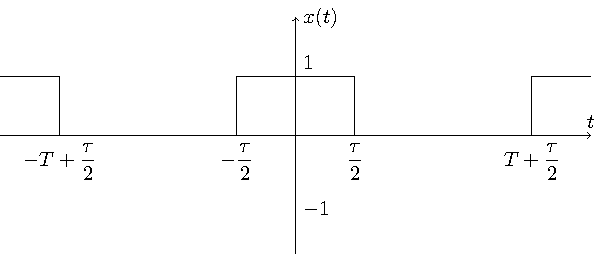
\includegraphics{onda-quadra-3.pdf}%
\end{figure}

Si vuole descrivere l'espansione  di Fourier della derivata di questo segnale. Si esprime come la differenza tra due gradini:
\begin{gather*}
    x(t)=\displaystyle\sum_{k=-\infty}^{+\infty}u\left(t-kT+\frac{\tau}{2}\right)-u\left(t-kT-\frac{\tau}{2}\right)\\
    \displaystyle\frac{\df}{\df t}x(t)=\sum_{k=-\infty}^{+\infty}\delta\left(t-kT+\frac{\tau}{2}\right)-\delta\left(t-kT-\frac{\tau}{2}\right)
\end{gather*}
Poiché per definizione la derivata di un gradino è l'impulso di Dirac. La derivata corrisponde ad una serie di impulsi nei punti dove l'onda quadra presenta delle discontinuità. 

\begin{figure}[H]%
    \centering
    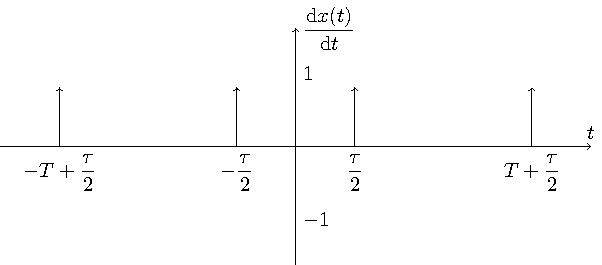
\includegraphics{serie-impulsi-1.pdf}%
\end{figure}

I coefficienti di Fourier corrispondenti alla derivata di $x$ risultano essere:
\begin{gather*}
    d_k=c_k\displaystyle\frac{2i\pi k}{T}=\frac{\tau}{T}\frac{2i\pi k}{T}\sinc\left({\frac{k\tau}{T}}\right)=\frac{\tau}{T}\frac{2i\pi k}{T}\frac{\sin(k\pi \tau/T)}{k\pi \tau/T}\\
    d_k=\displaystyle\frac{2i}{T}\sin\left(\frac{k\pi\tau}{T}\right)
\end{gather*}

Per un'onda quadra avente periodo $T$ pari al doppio della base delle finestre $\tau$: $T=2\tau$, i suoi coefficienti di Fourier risultano essere:
\begin{equation*}
    d_k=\displaystyle\frac{i}{\tau}\sin\left(\frac{k\pi}{2}\right)
\end{equation*}
Poiché $k\in\mathbb{Z}$, il valore dei coefficienti è o $\pm1$ o assume un valore nullo. 

Si calcolano tramite la definizione:
\begin{gather*}
    d_k=\displaystyle\int_{-\frac{T}{2}}^{\frac{T}{2}}\delta\left(t-kT+\frac{\tau}{2}\right)-\delta\left(t-kT-\frac{\tau}{2}\right)\df t=
    \int_{-\frac{T}{2}}^{\frac{T}{2}}\delta\left(t+\frac{\tau}{2}\right)-\delta\left(t-\frac{\tau}{2}\right)\df t\\
\end{gather*}
Poiché all'interno dell'intervallo di integrazione cade un singolo impulso

\subsection{Segnale Treno di Impulsi o Campionatore}

Questo segnale corrisponde ad una serie di impulsi di periodo $T$. Questo segnale è anche noto come segnale pettine o rastrelliera.  
\begin{equation*}
    x(t)=\pi(t)=\displaystyle\sum_{k=-\infty}^{+\infty}\delta(t-kT)
\end{equation*}
Permette di passare da un segnale analogico ad un segnale digitale, estraendo campioni ad intervalli regolari dal segnale in tempo continuo. 

\begin{figure}[H]%
    \centering
    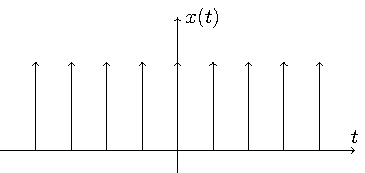
\includegraphics{rastrelliera.pdf}%
\end{figure}


Si calcolano i coefficienti dell'espansione di Fourier del segnale pettine. Si considera l'unico impulso che cade all'interno dell'intervallo di integrazione, centrato 
in $t=0$, per la proprietà di campionamento della delta e per l'area della delta si ottiene:
\begin{gather*}
    c_k=\displaystyle\frac{1}{T}\int_{-\frac{T}{2}}^{\frac{T}{2}}\delta(t)e^{-i\frac{2\pi kt}{T}}\df t=\frac{1}{T}\cancelto{1}{e^{-i{\frac{2\pi k0}{T}}}}\cancelto{1}{\int_{-\frac{T}{2}}^{\frac{T}{2}}\delta(t)\df t}\\
    c_k=\displaystyle\frac{1}{T}
\end{gather*}

Tutti i coefficienti della serie di Fourier della rastrelliera assumono lo stesso valore costante $1/T$. 

\subsection{Segnali Reali}
Se un segnale è reale, i suoi coefficienti possono essere espressi in un altro modo. Considerando la forma integrale dei coefficienti, e la formula di Eulero per gli 
esponenziali
\begin{gather*}
    c_k=\displaystyle\frac{1}{T}\int_{-\frac{T}{2}}^{\frac{T}{2}}x(t)\left[\cos\left(\frac{2\pi kt}{T}\right)-i\sin\left(\frac{2\pi kt}{T}\right)\right]\df t\\
    c_k=\displaystyle\frac{1}{T}\int_{-\frac{T}{2}}^{\frac{T}{2}}x(t)\cos\left(\frac{2\pi kt}{T}\right)\df t-\frac{i}{T}\int_{-\frac{T}{2}}^{\frac{T}{2}}x(t)\sin\left(\frac{2\pi kt}{T}\right)\df t
\end{gather*}
Si definiscono due coefficienti $a_k$ e $b_k$ pari alla parte reale ed immaginaria del coefficienti $c_k$:
\begin{gather*}
    c_k=a_k+ib_k\\
    a_k=\displaystyle\frac{1}{T}\int_{-\frac{T}{2}}^{\frac{T}{2}}x(t)\cos\left(\frac{2\pi kt}{T}\right)\df t\\
    b_k=\displaystyle-\frac{1}{T}\int_{-\frac{T}{2}}^{\frac{T}{2}}x(t)\sin\left(\frac{2\pi kt}{T}\right)\df t
\end{gather*}
I coefficienti $a_k$ sono pari, mentre i coefficienti $b_k$ sono dispari:
\begin{gather*}
    a_k=a_{-k}\\
    b_k=-b_{-k}\\
    c_{-k}=a_{-k}+ib_{-k}=a_{k}-ib_k=c_k^*
\end{gather*}
In forma polare si può esprimere come:
\begin{gather*}
    c_k=\rho_k e^{i\phi_k}\\
    c_{-k}=\rho_{-k}e^{i\phi{-k}}=\rho_k e^{-i\phi}=c_k^*
\end{gather*}

Un qualsiasi segnale reale può essere espresso come:
\begin{gather*}
    x(t)=\displaystyle\sum_{k=-\infty}^{-1}c_ke^{i\frac{2\pi kt}{T}}+c_0+\sum_{k=1}^{+\infty}c_ke^{i\frac{2\pi kt}{T}}=\sum_{k=1}^{+\infty}c_{-k}e^{-i\frac{2\pi kt}{T}}+c_0+\sum_{k=1}^{+\infty}c_ke^{i\frac{2\pi kt}{T}}\\
    \displaystyle\left(\sum_{k=1}^{+\infty}c_k^*e^{-i\frac{2\pi kt}{T}}+c_ke^{i\frac{2\pi kt}{T}}\right)+c_0=\left(\sum_{k=1}^{+\infty}\rho_k e^{-i\phi}e^{-i\frac{2\pi kt}{T}}+\rho_ke^{i\phi}e^{i\frac{2\pi kt}{T}}\right)+c_0\\
    x(t)=\displaystyle\sum_{k=1}^{+\infty}\rho_k \left(e^{i\left(\frac{2\pi kt}{T}+\phi_k\right)}+e^{-i\left(\frac{2\pi kt}{T}+\phi_k\right)}\right)+c_0=\displaystyle c_0+\sum_{k=1}^{+\infty}2\rho_k\cos\left(\frac{2\pi kt}{T}+\phi_k\right)
\end{gather*}
Questo rappresentazione è possibile solo per segnali $x$ reali. 
Considerando le formule del coseno della somma si può esprimere come:
\begin{gather*}
    \displaystyle c_0+\sum_{k=1}^{+\infty}2\rho_k\cos\left(\frac{2\pi kt}{T}+\phi_k\right)=
    c_0+\sum_{k=1}^{+\infty}2\rho_k\cos(\phi_k)\cos\left(\frac{2\pi kt}{T}\right)-2\rho_k\sin(\phi_k)\sin\left(\frac{2\pi kt}{T}\right)\\
    x(t)=\displaystyle c_0+2\sum_{k=1}^{+\infty}a_k\cos\left(\frac{2\pi kt}{T}\right)-b_k\sin\left(\frac{2\pi kt}{T}\right)\\
    a_k=\displaystyle\frac{1}{T}\int_{-\frac{T}{2}}^{\frac{T}{2}}x(t)\cos\left(\frac{2\pi kt}{T}\right)\df t\\
    b_k=\displaystyle-\frac{1}{T}\int_{-\frac{T}{2}}^{\frac{T}{2}}x(t)\sin\left(\frac{2\pi kt}{T}\right)\df t
\end{gather*}
Se il segnale $x$ è reale e pari, allora i coefficienti $b_k$ sono nulli, se il segnale è immaginario e dispari, i coefficienti $a_k$ sono nulli. 
Per cui i coefficienti $c_k$ di Fourier di un segnale reale e pari sono pari e reali, i coefficienti $c_k$ di Fourier di un segnale immaginario e 
dispari sono immaginari e dispari. 

\clearpage

\section{Trasformata di Fourier}
Quando si trattano segnali non periodici, non si possono esprimere mediante una serie di Fourier, quindi si analizzano mediante la trasformata di Fourier. 
La trasformata di Fourier si può applicare solamente a segnali impulsivi. Segnali impulsivi sono definiti dalla seguente espressione:
\begin{equation*}
    \displaystyle\int_{-\infty}^{+\infty}|x(t)|\df t\neq\infty
\end{equation*}
Come la serie di Fourier la trasformata di Fourier è uno strumento per analizzare i segnali. Questi segnali possono essere nel dominio del tempo $x(t)$ o dominio 
della frequenza $X(f)$. La trasformata è quindi un funzionale che dipende dalla variabile della frequenza, non più dalla variabile del tempo del segnale originale $x(t)$. 
La trasformata $X(f)$ è univoca per ogni segnale $x(t)$ nel tempo. Questa trasformata associa univocamente un segnale nel dominio del tempo ad un segnale nel dominio della 
frequenza:   
\begin{equation*}
    \mathscr{F}\{x(t)\}=X(f)
\end{equation*}

Ricordando la serie di un segnale periodico $x$ di periodo $T$:
\begin{gather*}
    x(t)=\displaystyle\sum_{k=-\infty}^{+\infty}c_ke^{i\frac{2\pi kt}{T}}
\end{gather*}
Nello spazio vettoriale dei segnali periodico è stato definito il prodotto scalare:
\begin{equation*}
    \langle x_1(t),\;x_2(t)\rangle=\displaystyle\frac{1}{T}\int_{-\frac{T}{2}}^{\frac{T}{2}}x_1(t)x_2^*(t)\df t
\end{equation*}
Nello spazio vettoriale di Fourier, la base ortonormale è formata da tutte le armonica:
\begin{gather*}
    \langle e^{i\frac{2\pi kt}{T}},\;e^{i\frac{2\pi nt}{T}}\rangle=\begin{cases}
        0&\forall k\neq n\\
        1&\forall k=n
    \end{cases}
\end{gather*} 
Da queste armoniche si può ricavare il coefficiente di ordine $k$ di un qualsiasi segnale periodico di periodo $T$:
\begin{equation*}
    c_k=\displaystyle\frac{1}{T}\int_{-\frac{T}{2}}^{\frac{T}{2}}x(t)e^{-i\frac{2\pi kt}{T}}\df t
\end{equation*}



Si considerano per semplicità tutti i segnali trattati come impulsivi. Per cui non sarà necessario dimostrare l'esistenza della trasformata di un certo segnale $x(t)$ 
non necessariamente periodico. Si vuole rappresentare questo segnale in modo equivalente alla serie di Fourier. Per rappresentare questo segnale sono necessarie un numero 
infinito non numerabile di armoniche, per cui si considera un integrale, dove il coefficiente dipende dalla variabile dell'integrale. E l'armonica non dipende dal parametro 
$k$, ma dalla stessa variabile dell'integrale:
\begin{equation*}
    x(t)=\displaystyle\int_{-\infty}^{+\infty}X(f)e^{2i\pi tf}df
\end{equation*}
Il segnale si esprime quindi tramite un insieme infinito non numerabile di armoniche, sempre uguali per ogni segnale. Per cui la differenza tra due segnali, come per 
l'espansione di Fourier, è il peso di ogni armonica $X(f)$. Bisogna comunque dimostrare che queste armoniche siano una base ortonormale in questo spazio di Fourier. Si 
introduce il prodotto scalare nello spazio dei segnali impulsivi:
\begin{equation*}
    \langle x_1(t),\;x_2(t)\rangle=\displaystyle\int_{-\infty}^{+\infty}x_1(t)x_2^*(t)\df t
\end{equation*}
Questo prodotto scalare corrisponde alla correlazione tra due segnali a ritardo nullo. 

Per determinare se due armoniche di frequenze diverse $f_1$ e $f_2$ sono una base si considera il loro prodotto scalare:
\begin{gather*}
    \langle e^{2i\pi f_1t},\;e^{2i\pi f_2t}\rangle=\displaystyle\lim_{\Delta t\to\infty}\int_{-\frac{\Delta t}{2}}^{+\frac{\Delta t}{2}}e^{2i\pi f_1t}e^{-2i\pi f_2t}\df t\\
    \displaystyle\lim_{\Delta t\to\infty}\left[\frac{e^{2i\pi(f_1-f_2)t}}{2i\pi(f_1-f_2)}\right]^{\frac{\Delta t}{2}}_{-\frac{\Delta t}{2}}=\lim_{\Delta t\to\infty}
    \Delta t\frac{\sin(\pi(f_1-f_2)\Delta t)}{\pi(f_1-f_2)\Delta t}\\
    \displaystyle\lim_{\Delta t\to\infty}\Delta t\,\sinc(\Delta t(f_1-f_2))
\end{gather*}
Per $\Delta t\to\infty$, la sinc diventa un impulso tempo continuo:
\begin{equation*}
    \langle e^{2i\pi f_1t},\;e^{2i\pi f_2t}\rangle=\delta(f_1-f_2)
\end{equation*}
Per cui tutte le armoniche di frequenza diversa hanno prodotto scalare nullo, e solo due armoniche di frequenza uguale hanno prodotto scalare di valore unitario. 
Bisogna dimostrare che i coefficienti trasformata di Fourier $X(f)$ si ottengono analogamente ai coefficienti $c_k$:
\begin{gather*}
    X(f)=\langle x(t),\;e^{2i\pi ft}\rangle=\displaystyle\int_{-\infty}^{+\infty}x(t)e^{-2i\pi ft}\df t
\end{gather*}
Nello spazio di Fourier si può poi analizzare la banda di un segnale, ovvero il contenuto informativo rispetto alla frequenza. Quest'informazione è necessaria per poter 
trasmettere un determinato segnale. I due domini del tempo e della frequenza sono due domini separati. 
Il nucleo o kernel della trasformata di Fourier corrisponde all'armonica, ovvero il componente esponenziale complesso nell'integrale. 

\subsection{Trasformate Notevoli}

Dato un segnale finestra:
\begin{gather*}
    x(t)=\rect\displaystyle\left(\frac{t}{\tau}\right)\\
    X(f)=\displaystyle\int_{-\infty}^{+\infty}\rect\left(\frac{t}{\tau}\right)e^{-2i\pi ft}\df t=\left[\frac{e^{-2i\pi ft}}{2i\pi ft}\right]^{+\frac{\tau}{2}}_{-\frac{\tau}{2}}\\
    \displaystyle\frac{e^{-i\pi f\tau}-e^{-i\pi f\tau}}{-2i\pi f}=\frac{\sin(\pi f\tau)}{\pi f}=\tau\,\sinc(f\tau)
\end{gather*}
Quindi la trasformata di un segnale finestra di base $\tau$ è un seno cardinale moltiplicato per la base, di argomento moltiplicato per la base:
\begin{gather*}
    x(t)=\rect\displaystyle\left(\frac{t}{\tau}\right)\rightarrow X(f)=\tau\,\sinc(f\tau)
\end{gather*}
La trasformata in $f=0$, corrisponde al valore medio del segnale finestra:
\begin{equation*}
    X(0)=\displaystyle\int_{-\frac{\tau}{2}}^{\frac{\tau}{2}}\df t=\tau
\end{equation*}
%% grafo
Questa proprietà si chiama teorema del valor medio. Ovvero per ogni segnale $x$, la trasformata per la frequenza nulla $f=0$ corrisponde al valore medio del segnale. 



Dato un segnale impulso di Dirac:
\begin{gather*}
    x(t)=\delta(t)\\
    X(f)=\displaystyle\int_{-\infty}^{+\infty}\delta(t)e^{-2i\pi ft}\df t=1
\end{gather*}
Per la proprietà di campionamento dell'impulso e per l'area dell'impulso, si ottiene che la trasformata di Fourier dell'impulso è sempre costante è unitario per ogni frequenza. 


Tanto più è limitato nel tempo, tanto più è largo il contenuto spettrale o la banda del segnale. Dove lo spettro di un segnale indica la sua trasformata di Fourier 
$\mathscr{F}$. 


Dato un segnale costante:
\begin{gather*}
    x(t)=1\\
    X(f)=\displaystyle\int_{-\infty}^{+\infty}e^{-2i\pi ft}\df t=\delta (f)
\end{gather*}
Analogamente al prodotto scalare tra due armoniche. 
Tanto più è esteso un segnale nel dominio del tempo, tanto più è limitato nel domino della frequenza. 


Dato il segnale impulso traslato:
\begin{gather*}
    x(t)=\delta (t-t_0)\\
    X(f)=\displaystyle\int_{-\infty}^{+\infty}\delta(t-t_0)e^{-2i\pi ft}\df t=e^{-2i\pi ft_0}
\end{gather*}
Dato il segnale armonica di frequenza $f_0$:
\begin{gather*}
    x(t)=e^{2i\pi f_0t}\\
    X(f)=\displaystyle\int_{-\infty}^{+\infty}e^{2i\pi(f_0-f)t}\df t=\delta(f_0-f)
\end{gather*}
Analogamente al prodotto scalare tra due armoniche di frequenza diversa. 


Dato il segnale coseno:
\begin{gather*}
    x(t)=\cos(2\pi f_0t)\\
    X(f)=\displaystyle\frac{1}{2}\int_{-\infty}^{+\infty}\left(e^{2i\pi f_0t}+e^{-2i\pi f_0t}\right)e^{-2i\pi ft}\df t=\frac{\delta(f-f_0)+\delta(f+f_0)}{2}\\
    x(t)=\cos(2\pi f_0t)\rightarrow X(f)=\displaystyle\frac{\delta(f-f_0)+\delta(f+f_0)}{2}
\end{gather*}
Nella notazione di Fourier un coseno viene rappresentato come due frequenze $\pm f_0$. 
Analogamente per il seno:
\begin{gather*}
    x(t)=\sin(2\pi f_0t)\\
    X(f)=\displaystyle\int_{-\infty}^{+\infty}\frac{1}{2i}(e^{2i\pi f_0t}-e^{-2i\pi f_0t})e^{-2i\pi ft}\df t=\frac{\delta (f-f_0)-\delta(f+f_0)}{2i}
\end{gather*}
Dato un coseno di ampiezza $A$ con un anticipo di fase $\phi$: 
\begin{gather*}
    x(t)=A\cos(2\pi f_0t+\phi)\\
    X(f)=\displaystyle\frac{A}{2}\int_{-\infty}^{+\infty}\left(e^{2i\pi f_0t}e^{i\phi}+e^{-2i\pi f_0t}e^{-i\phi}\right)e^{-2i\pi ft}\df t\\
    X(f)=\frac{A\delta(f-f_0)e^{i\phi}+A\delta(f+f_0)e^{-i\phi}}{2}
\end{gather*}

\subsection{Proprietà di Linearità}

La trasformata di Fourier è un operatore lineare. Dati due segnali $x(t)$ e $y(t)$:
\begin{gather*}
    x(t)\to X(f)\\
    y(t)\to Y(f)\\
    ax(t)+by(t)=\displaystyle\int_{-\infty}^{+\infty}(ax(t)+by(t))e^{-2i\pi ft}\df t\\
    a\int_{-\infty}^{+\infty}x(t)e^{-2i\pi ft}\df t+b\int_{-\infty}^{+\infty}y(t)e^{-2i\pi ft}\df t= 
    aX(f)+bY(f)
\end{gather*}

\subsection{Proprietà di Dualità}

La trasformata di Fourier accoppia due segnali nei due domini. Se la trasformata di un segnale $x$ nel tempo è una funzione $y$ nella frequenza, la trasformata di un segnale $y$ 
nel tempo è un segnale $x$ nella frequenza, di variabile opposta $-f$.

Per dimostrare questa proprietà si considerano la formula di trasformazione:
\begin{equation*}
    X(f)=\displaystyle\int_{-\infty}^{+\infty}x(t)e^{-2i\pi ft}\df t
\end{equation*}
E la formula di antitrasformazione:
\begin{equation*}
    x(t)=\displaystyle\int_{-\infty}^{+\infty}X(f)e^{2i\pi ft}\df f
\end{equation*}

Data la trasformata di un segnale $x(t)$ $X(f)$, per riportarla nel dominio del tempo, si considera l'integrale di trasformazione di $X(t)$:
\begin{gather*}
    \displaystyle\int_{-\infty}^{+\infty}X(t)e^{-2i\pi ft}\df t
\end{gather*}
Si considera la sostituzione $f=t'$ e $t=f'$, l'integrale diventa l'integrale di antitrasformazione:
\begin{equation*}
    \displaystyle\int_{-\infty}^{+\infty}X(f')e^{-2i\pi f't'}\df f'=x(-t')
\end{equation*}
Allora:
\begin{gather*}
    \mathscr{F}\{x(t)\}= X(f)\\
    \mathscr{F}\{X(t)\}=x(-f)
\end{gather*}

\subsection{Proprietà di Scala}

Si considera la trasformata di un segnale:
\begin{gather*}
    x(at)\to\displaystyle\int_{-\infty}^{+\infty}x(at)e^{-2i\pi ft}\df t\\
    t'=at\\
    \displaystyle\frac{1}{a}\int_{-\infty}^{+\infty}x(t')e^{-2i\pi \frac{f}{a}t'}\df t'=\frac{1}{a}X\left(\frac{f}{a}\right)
\end{gather*}
Se $a=-1$, la trasformata corrisponde a:
\begin{gather*}
    \displaystyle\int_{-\infty}^{+\infty}x(-t)e^{-2i\pi ft}\df t\\
    t'=-t\\
    \displaystyle\int_{-\infty}^{+\infty}x(t')e^{-2i\pi(- f)t'}\df t'=X(-f)
\end{gather*}
Per cui quando $a<0$:
\begin{gather*}
    x(at)\to\displaystyle\int_{-\infty}^{+\infty}x(t)e^{-2i\pi ft}\df t\\
    t'=at\\
    \displaystyle\frac{1}{|a|}\int_{-\infty}^{+\infty}x(t')e^{-2i\pi \left(-\frac{f}{a}\right)t'}\df t'=\frac{1}{|a|}X\left(-\frac{f}{a}\right)
\end{gather*}
Per cui in generale dato un segnale scalato di un fattore $a$, la sua trasformata è:
\begin{gather*}
    \mathscr{F}\{x(at)\}=\displaystyle\frac{1}{|a|}X\left(\frac{f}{a}\right)
\end{gather*}

\subsection{Ulteriori Trasformate Notevoli}

Si considera la trasformata del segnale gaussiano:
\begin{gather*}
    x(t)=e^{-\alpha t^2}\\
    X(f)=\displaystyle\int_{-\infty}^{+\infty}e^{-\alpha t^2}e^{-2i\pi ft}\df t=\int_{-\infty}^{+\infty}e^{-\alpha\left(\frac{2i\pi ft}{\alpha} + t^2\right)}\df t\\
    \displaystyle\int_{-\infty}^{+\infty}e^{-\alpha\left[t^2+\frac{2i\pi ft}{\alpha}+\left(\frac{i\pi f}{\alpha}\right)^2-+\left(\frac{i\pi f}{\alpha}\right)^2\right]}\df t\\
    e^{-\frac{\pi^2f^2}{\alpha}}\displaystyle\int_{-\infty}^{+\infty}e^{-\alpha\left(t+\frac{i\pi f}{\alpha}\right)^2}\df t
\end{gather*}
Si applica la sostituzione $\tau=\sqrt{\alpha}(t+i\pi f/\alpha)$, l'integrale diventa allora:
\begin{gather*}
    e^{-\frac{\pi^2f^2}{\alpha}}\displaystyle\int_{-\infty}^{+\infty}e^{-\tau^2}\frac{\df\tau}{\sqrt{\alpha}}=e^{-\frac{\pi^2f^2}{\alpha}}\sqrt{\frac{\pi}{\alpha}}\\
    X(f)=\sqrt{\frac{\pi}{\alpha}}e^{-\frac{\pi^2f^2}{\alpha}}
\end{gather*}

In forma normalizzata la gaussiana si esprime direttamente rispetto alla deviazione standard $\sigma$ e alla sua varianza $\sigma^2$:
\begin{gather*}
    x(t)=e^{-\frac{t^2}{2\sigma^2}}\\
    X(f)=\sqrt{2\pi}\sigma e^{-2\pi^2\sigma^2f^2}
\end{gather*}
L'area sottesa dalla gaussiana risulta essere il valor medio, esprimibile tramite il valore della trasformata per $f=0$:
\begin{equation*}
    X(0)=\sqrt{2\pi}\sigma
\end{equation*}
La gaussiana è una delle pochissime funzioni che si auto-trasforma. 

Si determina la trasformata dell'esponenziale unilatero:
\begin{gather*}
    x(t)=e^{-\alpha t}u(t)\\
    X(f)=\displaystyle\int_{-\infty}^{+\infty}e^{-\alpha t}u(t)e^{-2i\pi ft}\df t=\int_0^{+\infty}e^{-(2i\pi f+\alpha)t}\df t\\
    \left[\displaystyle\frac{e^{-(2i\pi f+\alpha)t}}{-(\alpha+2i\pi f)}\right]^{+\infty}_0=0+\frac{1}{\alpha+2i\pi f}\\
    X(f)=\frac{1}{\alpha+ 2i\pi f}
\end{gather*}
Il modulo quadro del segnale corrisponde ad una Lorentziana, una funzione simile ad una gaussiana: 
\begin{equation*}
    \left|X(f)\right|^2=\frac{1}{\alpha^2+4\pi^2f^2}
\end{equation*}
\begin{figure}[H]%
    \centering
    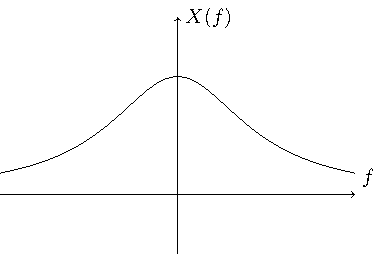
\includegraphics{lorentziana.pdf}%
\end{figure}


Dato il segnale esponenziale del modulo. Si può esprimere il segnale come due esponenziali unilateri:
\begin{figure}[H]%
    \centering
    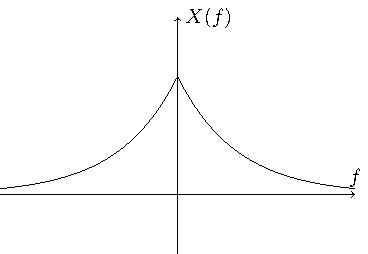
\includegraphics{esponenziali-unilateri.pdf}%
\end{figure}
\begin{gather*}
    x_1(t)=e^{-\alpha|t|}\\
    x_1(t)=x(t)+x(-t)\\
    X_1(f)=X(f)+X(-f)=\displaystyle\frac{1}{\alpha+2i\pi f}+\frac{1}{\alpha-2i\pi ft}=\frac{2\alpha}{\alpha^2+4\pi^2f^2}
\end{gather*}
Per cui la sua trasformata corrisponde alla Lorentziana. 


Dato il segnale Lorentziana, si può calcolare la sua trasformata tramite la proprietà di dualità della trasformata: 
\begin{gather*}
    x_2(t)=\displaystyle\frac{1}{\alpha+2i\pi t}\\
    X(f)=x(-f)=e^{\alpha f}u(-f)
\end{gather*}



Dato il segnale gradino, si può esprimere come il limite di un esponenziale unilatero:
\begin{equation*}
    x_3(t)=u(t)=\lim_{\alpha\to0}e^{-\alpha t}{u(t)}
\end{equation*}
Poiché non è un segnale impulsivo, questo risultato non rappresenta la trasformata su tutte le frequenze. 
\begin{gather*}
    X(f)=\displaystyle\lim_{\alpha\to0}\frac{1}{\alpha+2i\pi f}=\frac{1}{2i\pi f}
\end{gather*}
Razionalizzando l'argomento del limite si osserva come il risultato ottenuto per frequenze nulle perda informazioni sulla trasformata:
\begin{gather*}
    \displaystyle\lim_{\alpha\to0}\frac{1}{\alpha+2i\pi f}=\lim_{\alpha\to0}\left(\frac{\alpha}{\alpha^2+4\pi^2f^2}-\frac{2i\pi f}{\alpha^2+4\pi^2f^2}\right)
\end{gather*}


Per cui si esprime la trasformata di un gradino come il limite ottenuto sommato ad una costante $A$ moltiplicata per l'impulso, per considerare il valore della trasformata 
per frequenze nulle: 
\begin{gather*}
    X(f)=\displaystyle\lim_{\alpha\to0}\frac{1}{\alpha+2i\pi f}=\frac{1}{2i\pi f}+\delta(f)A
\end{gather*}
Il fattore $A$ si ottiene integrando il fattore che si annulla nel limite:
\begin{gather*}
    A=\displaystyle\int_{-\infty}^{+\infty}\frac{\alpha}{\alpha^2+4\pi^2f^2}\df f=\int_{-\infty}^{+\infty}\frac{1}{\alpha\left(1+\frac{4\pi^2f^2}{\alpha^2}\right)}\df f\\
    f'=\displaystyle\frac{2\pi f}{\alpha}\\
    \displaystyle\frac{1}{\alpha}\frac{\alpha}{2\pi}\int_{-\infty}^{+\infty}\frac{1}{1+f'^2}\df f'=\left[\frac{1}{2\pi}\arctan f'\right]^{+\infty}_{-\infty}=\frac{1}{2\pi}\left[\frac{\pi}{2}-\left(-\frac{\pi}{2}\right)\right]=\frac{1}{2}
\end{gather*}
Per cui la trasformata di un gradino, segnale non impulsivo, risulta essere:
\begin{equation*}
    X_3(f)=\displaystyle\frac{1}{2}\delta(f)+\frac{1}{2i\pi f}
\end{equation*}


Si considera il segnale segno, e si vuole determinare la sua trasformata:
\begin{gather*}
    x_4(t)=\mbox{sign}(t)=u(t)-u(-t)\\
    X_4(f)=X_3(f)-X_3(-f)=\displaystyle\frac{1}{2}\delta(f)+\frac{1}{2i\pi f}-\frac{1}{2}\delta(f)+\frac{1}{2i\pi f}=\frac{1}{i\pi f}
\end{gather*}

\subsection{Funzioni di Trasferimento}

Per determinare la risposta impulsiva di un filtro si considera in entrata un impulso, ma inviare un segnale infinitesimo in un sistema non è semplice. Per cui generalmente 
si inserisce in ingresso un armonica a frequenza costante $f_0$:
\begin{gather*}
    y(t)=\displaystyle\int_{-\infty}^{+\infty}h(t)e^{2i\pi f_0(t-\tau)}\df\tau\\
    e^{2i\pi f_0t}\displaystyle\int_{-\infty}^{+\infty}h(t)e^{-2i\pi f_0\tau}\df\tau=e^{2i\pi f_0t}H(f_0)
\end{gather*}
Si definisce la risposta impulsiva nel dominio della frequenza la funzione di trasferimento del sistema. I filtri sono sistemi che filtrano nel dominio delle frequenze. 

Per cui un filtro è caratterizzato dalla risposta impulsiva o dalla sua funzione di trasferimento, che indica quale frequenze vengono eliminate dal filtro. 




Una Lorentziana è un segnale dove la maggior parte del contenuto informativo è all'interno di un'intervallo finito. Si definiscono quindi dei segnali passa basso, 
ovvero dei segnali il cui contenuto informativo è presente nell'intorno dell'origine. Se un filtro ha funzione di trasferimento passa basso, allora si definisce segnale 
passa basso. La banda del segnale è legata alla frequenza massima $f_{max}$, non è necessario sia una finestra in frequenza, una qualsiasi funzione che assume valori nulli 
per frequenze maggiori della frequenza massima è una funzione passa basso valida per essere funzione di trasferimento di un filtro. 

Tutti i segnali inviati per cavi presentano una banda base, ovvero sono segnali passa basso. 


Esistono altri segnali chiamati passa banda, o modulati. Il segnale è centrato in una frequenza $\pm f_0$, chiamata portante. Si usano per la trasmissioni di segnali 
che vengono inviati nell'etere, tutti questi segnali devono essere modulati. 

\subsection{Traslazione nel Tempo}

Data la trasformata di Fourier di un segnale tempo continuo, è nota anche la trasformata del segnale ritardato o anticipato:
\begin{gather*}
    \mathscr{F}\{x(t)\}=X(f)\\
    \mathscr{F}\{x(t-t_0)\}=\displaystyle\int_{-\infty}^{+\infty}x(t-t_0)e^{-2i\pi ft}\df t\\
    \tau=t-t_0\\
    \displaystyle\int_{-\infty}^{+\infty}x(\tau)e^{-2i\pi f(\tau+t_0)}\df\tau=e^{-2i\pi ft_0}\int_{-\infty}^{+\infty}x(\tau)e^{-2i\pi f\tau}\df\tau=e^{-2i\pi ft_0}X(f)
\end{gather*}

Data una gaussiana traslata nel tempo:
\begin{gather*}
    x(t)=e^{-\alpha(t-t_0)^2}\\
    X(f)=\displaystyle\sqrt{\frac{\pi}{\alpha}}e^{-\left(\frac{\pi^2f^2}{\alpha}+2i\pi ft_0\right)}
\end{gather*}

\subsection{Traslazione in Frequenza}

Questa proprietà si indica anche come proprietà di modulazione. 
Si considera un segnale moltiplicato per un armonica di frequenza costante $f_0$:
\begin{gather*}
    \mathscr{F}\left\{e^{2i\pi f_0t}x(t)\right\}=\displaystyle\int_{-\infty}^{+\infty}x(t)e^{-2i\pi(f-f_0)t}\df t=X(f-f_0)
\end{gather*}

Quest'operazione si chiama modulazione di ampiezza (AM). Il segnale trasmesso corrisponde ad un coseno di ampiezza pari al segnale originario.
\begin{gather*}
    \mathscr{F}\{x(t)\cos(2\pi f_0t)\}=\displaystyle\frac{1}{2}\int_{-\infty}^{+\infty}x(t)\left[e^{2i\pi f_0t}+e^{-2i\pi f_0t}\right]e^{-2i\pi ft}\df t\\
    \frac{1}{2}\displaystyle\int_{-\infty}^{+\infty}x(t)e^{-2i\pi(f-f_0)t}\df t+\frac{1}{2}\int_{-\infty}^{+\infty}x(t)e^{-2i\pi (f+f_0)t}\df t=\frac{X(f-f_0)}{2}+\frac{X(f+f_0)}{2}
\end{gather*}

\subsection{Proprietà Operative della Trasformata}

\subsubsection{Proprietà della Derivazione}

La trasformata, nel trasportare una funzione da un dominio all'altro, può offrire una serie di semplificazioni ad operazioni come integrali e derivate nei due domini. Si vuole 
determinare la trasformata della derivata di un noto segnale $x$, di trasformata $X$. 

Si considera il segnale derivata $x_1$:
\begin{gather*}
    x_1(t)=\displaystyle\frac{\df}{\df t}x(t)\\
    X_1(f)=\displaystyle\int_{-\infty}^{+\infty}\left(\frac{\df}{\df t}x(t)\right)e^{-2i\pi ft}\df t
\end{gather*}
Si considera l'antitrasformata del segnale originale $x$ e si derivano entrambi i lati rispetto al tempo: 

\begin{gather*}
    x(t)=\displaystyle\int_{-\infty}^{+\infty}X(f)e^{2i\pi ft}\df f\\
    \displaystyle\frac{\df}{\df t}x(t)=\int_{-\infty}^{+\infty}2i\pi fX(f)e^{2i\pi ft}\df f=x_1
\end{gather*}
Quest'integrale rappresenta l'antitrasformata del segnale derivata $x_1$, per cui la sua trasformata può essere espressa come:
\begin{gather*} 
    X_1(t)=2i\pi fX(f)
\end{gather*}

\subsubsection{Duale della Derivazione}
Dato un segnale $x(t)$ e la sua trasformata $X(f)$, si dimostra che vale la proprietà duale della derivazione: 
\begin{gather*}
    x_1(t)=2i\pi tx(t)\\
    X_1(f)=\displaystyle\int_{-\infty}^{+\infty}2i\pi tx(t)e^{-2i\pi ft}\df t\\
    X(f)=\displaystyle\int_{-\infty}^{+\infty}x(t)e^{-2i\pi ft}\df t\\
    \displaystyle\frac{\df}{\df f}X(f)=\int_{-\infty}^{+\infty}-2i\pi t x(t)e^{2i\pi ft}\df t=-\int_{-\infty}^{+\infty}x_1(t)e^{2i\pi ft}\df t=-X_1(f)\\
    \displaystyle\frac{\df}{\df f}X(f)=-X_1(f)
\end{gather*}


Si considera il seguente segnale in frequenza:
\begin{gather*}
    X_1(f)=\displaystyle\frac{1}{(\alpha+2i\pi f)^2}
\end{gather*}
Per ottenere la trasformata del segnale, si considera il duale della proprietà della derivazione della trasformata. Si considera il segnale esponenziale unilatero e la sua 
trasformata:
\begin{gather*}
    x(t)=e^{-\alpha t}u(t)\\
    X(f)=\displaystyle\frac{1}{\alpha+2i\pi f}\\
    \displaystyle\frac{\df}{\df f}X(f)=\frac{-2i\pi}{(\alpha+2i\pi f)^2}\\
    X_1(f)=\displaystyle-\frac{1}{2i\pi}\frac{\df}{\df f}X(f)=-\frac{1}{2i\pi}(-2i\pi tx(t))=te^{-\alpha t}u(t)
\end{gather*}

\subsubsection{Prorpietà dell'Integrazione}

Dato un segnale $x$ di trasformata $X$, si considera il suo integrale fino ad un valore $\tau$, ciò equivale ad attuare una convoluzione con il gradino $u(t)$:
\begin{gather*}
    x_1(t)=\displaystyle\int_{-\infty}^{+\tau}x(\tau)\df\tau=\int_{-\infty}^{*\infty}u(t-\tau)x(\tau)\df\tau=x(t)*u(t)
\end{gather*}
Nel domino della frequenza la trasformata del segnale $x_1$ è quindi il prodotto tra la trasformata di $x$ e del segnale gradino:
\begin{gather*}
    X_1(f)=X(f)\left[\displaystyle\frac{1}{2}\delta(f)+\frac{1}{2i\pi f}\right]=\frac{1}{2}X(0)\delta(f)+\frac{X(f)}{2i\pi f}
\end{gather*}

\subsubsection{Proprietà del Coniugato}

Dato un segnale $x$ di trasformata $X$, si considera il suo coniugato $x*$, e si vuole calcolare la sua trasformata:
\begin{gather*}
    x_1(t)=x^*(t)\\
    X_1(f)=\displaystyle\int_{-\infty}^{+\infty}x^*(t)e^{2i\pi ft}\df t=\left(\int_{-\infty}^{+\infty}x(t)e^{-2i\pi ft}\df t\right)^*=X^*(-f)
\end{gather*}
La coniugazione ha quindi una simmetria hermitiana, nella trasformata di Fourier. 

\subsubsection{Proprietà della Correlazione}

Dato una una correlazione $z$ tra due segnali $x$ e $y$, si può esprimere come una convoluzione. Tramite il teorema della convoluzione e del coniugato, la sua trasformata può 
essere espressa come il prodotto tra due trasformate: 
\begin{gather*}
    z(t)=x(t)\otimes y(t)=\displaystyle\int_{-\infty}^{+\infty}x(t+\tau)y^*(\tau)\df\tau=x(t)*y^*(-t)\\
    Z(f)=X(f)\cdot Y^*(f)
\end{gather*}

\subsection{Finestra e Triangolo tramite Derivata}
Dato un segnale finestra e la sua trasformata:
\begin{gather*}
    x(t)=\rect\displaystyle\left(\frac{t}{T}\right)\\
    X(f)=T\sinc\displaystyle\left(Tf\right)
\end{gather*}
Si considera ora la derivata del segnale finestra. Questo segnale è costante per tutti valori eccetto per le discontinuità in $\pm T/2$, dove presenta una variazione istantanea. 
Esprimendola come due gradini, questa variazione viene espressa nella derivata come la differenza tra due impulsi, nota la derivata di un gradino: 
\begin{gather*}
    x(t)=u(t-T/2)-u(t+T/2)\\
    \displaystyle\frac{\df}{\df t}x(t)=\delta(t-T/2)-\delta(t+T/2)
\end{gather*}
La trasformata della derivata risulta essere:
\begin{gather*}
    X(f)=2i\pi fT\,\sinc(Tf)=\displaystyle2i\pi fT\frac{\sin(\pi Tf)}{\pi Tf}\\
    2i\sin(\pi Tf)=2i\frac{e^{i\pi Tf}-e^{-i\pi Tf}}{2i}\\
    X(f)=e^{i\pi Tf}-e^{-i\pi Tf}
\end{gather*}


Si considera ora un segnale triangolo di base $T$, e si attua un processo analogo. La sua derivata è quindi la differenza tra due finestre, poiché aumenta costantemente da 
$-T$ a $0$ e decresce costantemente da $0$ a $T$. 
\begin{gather*}
    x(t)=\mbox{tri}\displaystyle\left(\frac{t}{T}\right)\\
    \displaystyle\frac{\df}{\df t}x(t)=\frac{1}{T}\rect\left(\frac{t+T/2}{T}\right)-\frac{1}{T}\rect\left(\frac{t-T/2}{T}\right)\\
    X'(f)=2i\pi f\displaystyle\left(\frac{1}{T}T\sinc(Tf)e^{i\pi Tf}-\frac{1}{T}T\sinc(Tf)e^{-i\pi Tf}\right)\\
    2i\,\sinc(Tf)\sin(Tf)=\displaystyle2i\frac{\sin^2(Tf)}{\pi Tf}
\end{gather*}

Per ottenere la trasformata del segnale triangolo, si considera la trasformata della sua derivata:
\begin{gather*}
    X'(f)=2i\pi fX(f)\\
    X(f)=\displaystyle2i\frac{\sin^2(Tf)}{\pi fT}\frac{1}{2i\pi f}=T\,\sinc^2(Tf)
\end{gather*}
La derivata nel dominio del tempo corrisponde a moltiplicare nel dominio della frequenza per il fattore $2i\pi f$. 

\subsection{Teorema della Convoluzione}

Data la convoluzione tra due segnali $x$ e $y$:
\begin{gather*}
    x(t)*y(t)=\displaystyle\int_{-\infty}^{+\infty}x(t-\tau)y(\tau)\df\tau
\end{gather*}
Si esprime il segnale $y$ antitrasformata:
\begin{gather*}
    y(\tau)=\displaystyle\int_{-\infty}^{+\infty}Y(f)e^{2i\pi f\tau}\df f\\
    x(t)*y(t)=\displaystyle\int_{-\infty}^{+\infty}x(t-\tau)\left(\int_{-\infty}^{+\infty}Y(f)e^{2i\pi f\tau}\df f\right)\df\tau
\end{gather*}
Si inverte l'ordine di integrazione, possibile poiché i due integrali sono indipendenti tra di loro, e si applica la sostituzione $t'=t-\tau$: 
\begin{gather*}
    x(t)*y(t)=\displaystyle\int_{-\infty}^{+\infty}Y(f)\left(\int_{-\infty}^{+\infty}x(t-\tau)e^{2i\pi f\tau}\df\tau\right)\df f\\
    t'=t-\tau\\
    \int_{-\infty}^{+\infty}Y(f)e^{2i\pi ft}\left(\int_{-\infty}^{+\infty}x(t')e^{-2i\pi ft'}\df t'\right)\df f\\
    x(t)*y(t)=\displaystyle\int_{-\infty}^{+\infty}Y(f)X(f)e^{2i\pi ft}\df f
\end{gather*}

\subsection{Filtri}

I filtri sono sistemi ingresso-uscita caratterizzati da un'unica funzione chiamata risposta impulsiva $h(t)$, che permette di calcolare l'uscita come la convoluzione tra l'
entrata e la risposta impulsiva. Per cui considerando il teorema appena dimostrato, l'uscita si può rappresentare nel domino della frequenza più semplicemente come un prodotto:
\begin{gather*}
    y(t)=x(t)*h(t)=\displaystyle\int_{-\infty}^{+\infty}X(f)H(f)e^{2i\pi ft}\df f\\
    Y(f)=X(f)\cdot H(f)
\end{gather*}
Per cui si può rappresentare molto più semplicemente l'uscita di un sistema nel dominio della frequenza, ovvero analizzando lo spettro dell'uscita. 

Si considera un segnale $x$ in entrata ad un filtro $h$:
\begin{gather*}
    h(t)=\displaystyle\frac{1}{T}\sinc\left(\frac{t}{T}\right)\\
    x(t)=\cos(2\pi f_0t)
\end{gather*}
Per la proprietà di scala:
\begin{gather*}
    H(f)=\rect(Tf)\\
    X(f)=\displaystyle\frac{1}{2}\delta(f-f_0)+\frac{1}{2}\delta(f+f_0)\\
    Y(f)=\frac{1}{2}\rect(Tf)(\delta(f-f_0)+\delta(f+f_0))\\
    \displaystyle\frac{1}{2}\rect(Tf_0)\delta(f-f_0)+\frac{1}{2}\rect(-Tf_0)\delta(f+f_0)
\end{gather*}


Dato un sistema definito dall'espressione:
\begin{gather*}
    \displaystyle\frac{\df}{\df t}y(t)+\alpha y(t)=x(t)
\end{gather*}
Si può semplificare l'analisi passando per il domino della frequenza: 
\begin{gather*}
    2i\pi fY(f)+\alpha Y(f)=X(f)\\
    Y(f)=\displaystyle\frac{1}{\alpha+2i\pi f}X(f)
\end{gather*}
Quindi la funzione di trasferimento del sistema risulta essere:
\begin{gather*}
    H(f)=\displaystyle\frac{1}{\alpha+2i\pi f}
\end{gather*}
E la sua antitrasformata è la risposta impulsiva del sistema, in questo caso un esponenziale unilatero: 
\begin{gather*}
    h(t)=e^{-\alpha t}u(t)
\end{gather*}

\subsection{Teorema di Parseval}

Si considera una convoluzione $z$, ed il suo valore nell'origine:
\begin{gather*}
    z(t)=x(t)*y(t)=\displaystyle\int_{-\infty}^{+\infty}x(t-\tau)y(\tau)\df\tau=\int_{-\infty}^{+\infty}X(f)Y(f)e^{2i\pi ft}\df f\\
    z(t)=\displaystyle\int_{-\infty}^{+\infty}x(-\tau)y(\tau)\df\tau=\int_{-\infty}^{+\infty}X(f)Y(f)\df f 
\end{gather*}
Si considera ora la convoluzione tra $x(t)$ e $y^*(-t)$, sempre calcolata nell'origine
\begin{gather*}
    z(t)=\displaystyle\int_{-\infty}^{+\infty}x(\tau)y^*(-(t-\tau))\df\tau=\int_{-\infty}^{+\infty}X(f)Y^*(f)e^{2i\pi ft}\df f\\
    z(0)=\displaystyle\int_{-\infty}^{+\infty}x(\tau)y^*(\tau)\df\tau=\int_{-\infty}^{+\infty}X(f)Y^*(f)\df f
\end{gather*}
Se si considera $y=x$, allora la convoluzione diventa un'auto-convoluzione. Calcolata nell'origine corrisponde all'energia di un segnale:
\begin{gather*}
    z(0)=\displaystyle\int_{-\infty}^{+\infty}x(\tau)x^*(\tau)\df\tau=\int_{-\infty}^{+\infty}X(f)X^*(f)\df f\\
    E_x=\displaystyle\int_{-\infty}^{+\infty}|x(\tau)|^2\df\tau=\int_{-\infty}^{+\infty}|X(f)|^2\df f
\end{gather*}
Per cui l'energia di un segnale si calcola esattamente allo stesso modo sia nel dominio del tempo che nel dominio della frequenza. 

\subsection{Trasformata di Segnali Reali}

Se un segnale $x(t)$ è reale, la sua trasformata di Fourier, gode delle seguenti proprietà:
\begin{gather*}
    x(t)\in\mathbb{R}\\
    X(f)=\displaystyle\int_{-\infty}^{+\infty}x_1(t)e^{-2i\pi ft}\df t=\int_{-\infty}^{+\infty}x_1(t)\left[\cos(2\pi ft)-i\sin(2\pi ft)\right]\df t\\
    \displaystyle\int_{-\infty}^{+\infty}x_1(t)\cos(2\pi ft)\df t-i\int_{-\infty}^{+\infty}x_1(t)\sin(2\pi ft)\df t\\
    \Re\left\{X(f)\right\}=\displaystyle\int_{-\infty}^{+\infty}x_1(t)\cos(2\pi ft)\df t\\
    \Im\left\{X(f)\right\}=\displaystyle-\int_{-\infty}^{+\infty}x_1(t)\sin(2\pi ft)\df t
\end{gather*}
La parte reale della trasformata di un segnale reale è pari, mentre la sua parte immaginaria è dispari:
\begin{gather*}
    \Re\left\{X(-f)\right\}=\Re\left\{X(f)\right\}\\
    \Im\left\{X(-f)\right\}=-\Im\left\{X(f)\right\}
\end{gather*}
Per cui la trasformata di un segnale reale ha simmetria hermitiana:
\begin{gather*}
    X(-f)=\Re\{X(-f)\}+i\Im\{X(-f)\}=\Re\{X(f)\}-i\Im\{X(f)\}=X^*(f)
\end{gather*}
Se il segnale $x$ è reale e pari, allora la sua trasformata è anch'essa reale e pari, poiché $\Im\left\{X(f)\right\}=0$. 
Analogamente se $x$ è reale e dispari, allora la sua trasformata è puramente immaginaria e dispari, poiché $\Re\{X(f)\}=0$. 

\subsection{Trasformata di Segnali Periodici}

Data l'espansione di Fourier di un segnale periodico $x$, di periodo $T$:
\begin{gather*}
    x(t)=\displaystyle\sum_{k=-\infty}^{+\infty}c_ke^{2i\pi kt/T}
\end{gather*}
La sua trasformata di Fourier corrisponde ad un treno di impulsi, centrati nei multipli della frequenza naturale $f_0=1/T$, di ampiezza pari al valore del coefficiente $k-$
esimo: 
\begin{gather*}
    X(f)=\displaystyle\sum_{k=-\infty}^{+\infty}c_k\delta\left(f-\frac{k}{T}\right)
\end{gather*}
La trasformata di un segnale periodico è sempre un treno di impulsi, moltiplicati ciascuno per un coefficiente $c_k$.


Si considera la formula del coefficiente di Fourier:
\begin{gather*}
    c_k=\frac{1}{T}\displaystyle\int_{-T/2}^{T/2}x(t)e^{-2i\pi kt/T}\df t
\end{gather*}
Poiché considera un singolo componente nell'intervallo, si può ottenere lo stesso coefficiente, considerando il segnale $\dot x(t)$, replica del segnale $x(t)$ nel solo periodo 
centrato in $t=0$, e nullo fuori dal periodo:
\begin{gather*}
    c_k=\frac{1}{T}\displaystyle\int_{-T/2}^{T/2}\dot x(t)e^{-2i\pi kt/T}\df t=\frac{1}{T}\dot X\left(\frac{k}{T}\right)
\end{gather*}
Assume il valore della trasformata del segnale $\dot x$, rispetto alla frequenza $f_k=k/T$. 

Si dimostra in questo modo, nella sezione successiva, che il treno campionatore è uno dei pochi segnali che si auto-trasforma, insieme con la gaussiana. 

\clearpage

\section{Trasformata di Fourier Tempo Discreto}

Si considera un filtro descritto da una risposta impulsiva $h(t)$, definita come la risposta $y(t)=x(t)*h(t)$ corrispondente ad un impulso in entrata $x(t)=u(t)$. Se viene 
inserita un'armonica nel sistema:
\begin{gather*}
    x(t)=e^{2i\pi f_0t}\\
    y(t)=h(t)*x(t)=\displaystyle\int_{-\infty}^{+\infty}h(\tau)e^{2i\pi f_0(t-\tau)}\df\tau=e^{2i\pi f_0t}\int_{-\infty}^{+\infty}h(\tau)e^{2i\pi f_0\tau}\df\tau\\
    H(f)=\displaystyle\int_{-\infty}^{+\infty}h(\tau)e^{2i\pi f_0\tau}\df\tau\\
    y(t)=e^{2i\pi f_0t}H(f_0)
\end{gather*}
Si è definita la trasformata della risposta impulsiva la funzione di trasferimento del filtro. L'uscita del sistema in frequenza si esprime quindi come il prodotto 
tra le trasformate delle due entrate. Poiché agisce selettivamente sulle varie frequenze in entrata si definisce questo tipo di sistema filtro. 

Si considera ora un filtro tempo discreto, descritto da una risposta impulsiva $h[n]$, definita come nel continuo dall'uscita del sistema ad un impulso in entrata. L'uscita 
$y[n]$ di un sistema tempo discreto si ottiene come la convoluzione tra l'entrata $x[n]$ e la risposta impulsiva:
\begin{gather*}
    y[n]=x[n]*h[n]
\end{gather*}
Continuando le analogie con il tempo continuo, sarà quindi possibile riportare questa relazione in frequenza, considerando un'armonica tempo discreta in entrata:
\begin{gather*}
    x[n]=e^{2i\pi f_0nT}
\end{gather*}
Poiché spesso un segnale tempo discreto corrisponde ad un segnale tempo continuo $x(t)$ campionato ad intervalli regolari $T$, creando così una sequenza di valori equamente 
distribuiti rispetto al tempo $x[n]$. Per cui questo segnale viene definito rispetto al tempo di campionamento, periodico, $T$. Si considera ora l'uscita del sistema 
data quest'entrata:
\begin{gather*}
    y[n]=e^{2i\pi f_0nT}*h[n]=\displaystyle\sum_{k=-\infty}^{+\infty}h[k]e^{2i\pi f_0(n-k)T}=e^{2i\pi f_0nT}\displaystyle\sum_{k=-\infty}^{+\infty}h[k]e^{-2i\pi f_0k}
\end{gather*}
Si definisce quindi la trasformata di Fourier discreta come la sommatoria così ottenuta, equivalente alla funzione di trasferimento tempo discreto della risposta 
impulsiva $h[n]$:
\begin{gather*}
    H(f_0)=\displaystyle\sum_{k=-\infty}^{+\infty}h[k]e^{-2i\pi f_0kT}\\
    y[n]=e^{2i\pi g_0nT}H(f_0)
\end{gather*}
Analogamente al tempo continuo, il sistema filtra l'armonica in entrata rispetto alla funzione di trasferimento del sistema. 
La prima informazione ricavabile da questo processo è che la trasformata di Fourier di una sequenza di valori, il segnale in discreto, è una funzione continua, nella 
variabile $f_0$. Per cui dato un generico segnale $x[n]$, la sua trasformata si ottiene come:
\begin{gather*}
    \mathscr{F}\{x[n]\}=\displaystyle\sum_{k=-\infty}^{+\infty}x[k]e^{-2i\pi fkT}=X(f)
\end{gather*}
Questo segnale risultante è periodico e di periodo $1/T$, si dimostra considerando la trasformata ritardata di un fattore $1/T$:
\begin{gather*}
    X\left(\displaystyle f-\frac{1}{T}\right)=\displaystyle\sum_{k=-\infty}^{+\infty}x[k]e^{2i\pi (f-1/T)T}=\displaystyle\sum_{k=-\infty}^{+\infty}x[k]e^{-2\pi fkT}\cancelto{1}{e^{2i\pi k}}=X(f)
\end{gather*}
Per analizzare un segnale periodico in frequenza, si considera la frequenza normalizzata $\Phi$, definita come il prodotto tra la frequenza ed il reciproco del periodo:
\begin{gather*}
    \Phi=TF
\end{gather*}
La funzione di trasferimento può essere espressa come:
\begin{gather*}
    X(\Phi)=\displaystyle\sum_{k=-\infty}^{+\infty}x[k]e^{-2i\pi k\Phi}
\end{gather*}
La funzione misurata rispetto alla frequenza normalizzata ha periodo unitario. 
Se la trasformata tempo discreta è un segnale periodico rispetto alla frequenza, allora per confronto diretto è la sua stessa rappresentazione di Fourier, nel dominio della 
frequenza di periodo $1/T$:
\begin{gather*}
    X(f)=\displaystyle\sum_{k=-\infty}^{+\infty}x[k]e^{-2i\pi kfT}=\sum_{k=-\infty}^{+\infty}c_ke^{-2i\pi kfT}\\
    c_k=x[k]
\end{gather*}
La sequenza stessa coincide esattamente con i coefficienti della serie di Fourier del segnale trasformata. Si considera ora la definizione di un coefficiente di Fourier, 
per ottenere la relazione inversa, ovvero l'antitrasformata dal dominio della frequenza al dominio tempo discreto:
\begin{gather*}
    c_k=\displaystyle T\int_{-1/2T}^{1/2T}X(f)e^{2i\pi kfT}\df f=x[k]
\end{gather*}

\subsection{Trasformate Notevoli}

Si considera un impulso discreto $\delta[n]$, e si vuole calcolare la sua trasformata di Fourier tramite la definizione:
\begin{gather*}
    X(f)=\displaystyle\sum_{k=-\infty}^{+\infty}\delta[k]e^{2i\pi fkT}=\delta[0]e^{-2i\pi 0fT}=1
\end{gather*}
Poiché l'unico campione non nullo dell'impulso si trova in $k=0$, e l'armonica assume valore unitario. Quindi la trasformata assume valore unitario e costante. 


Si considera un segnale discreto, analogo ad una finestra traslata, che presenta campioni di valore unitario da $k=0$, fino a $k=N-1$. La sua trasformata è quindi:
\begin{gather*}
    X(f)=\displaystyle\sum_{k=0}^{N-1}1\cdot e^{-2i\pi kfT}
\end{gather*}
Corrisponde ad una somma di potenze di base $x=e^{-2i\pi fT}$, per cui converge ad un valore:
\begin{gather*}
    X(f)=\displaystyle\sum_{k=0}^{N-1}x^k=\frac{1-x^N}{1-x}=\frac{1-e^{-2i\pi NfT}}{1-e^{-2i\pi fT}}\\
    \frac{e^{-i\pi NfT}}{e^{-i\pi fT}}\frac{e^{i\pi NfT}-e^{-i\pi NfT}}{e^{i\pi fT}-e^{-i\pi fT}}=e^{-i\pi(N-1)fT}\frac{\sin(\pi fNT)}{\sin(\pi fT)}
\end{gather*}
Il modulo della trasformata corrisponde ad un rapporto tra due seni:
\begin{gather*}
    |X(f)|=\displaystyle\frac{\sin(\pi fNT)}{\sin(\pi fT)}
\end{gather*}
Il segnale si annulla ogni multiplo del fattore $1/NT$, un valore massimo $N$ per $f=0$, ed ha un periodo di $1/T$:
\begin{figure}[H]%
    \centering
    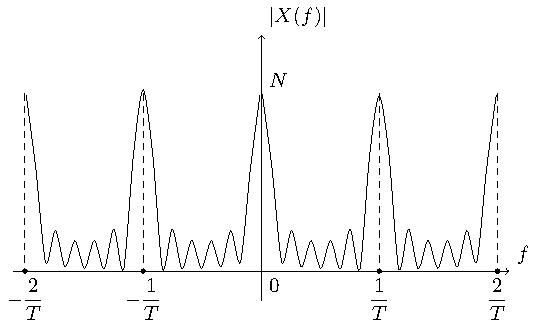
\includegraphics{trasformata-discreta-1.pdf}%
\end{figure}


Si considerano due campioni in $k=0,1$. La trasformata corrispondente si ottiene come:
\begin{gather*}
    x[n]=\delta[n]+\delta[n-1]\\
    X(f)=\displaystyle\sum_{k=0}^1e^{-2i\pi kfT}=1+e^{-2i\pi fT}=e^{-i\pi fT}\left(e^{i\pi fT}+e^{-i\pi fT}\right)=2e^{-i\pi fT}\cos(\pi fT)\\
    |X(f)|=2\cos(\pi fT)
\end{gather*}
\begin{figure}[H]%
    \centering
    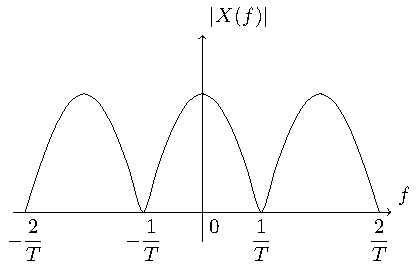
\includegraphics{trasformata-discreta-2.pdf}%
\end{figure}


Questa trasformata corrisponde ad un filtro passa basso, ovvero filtra le alte frequenze, e permette alle basse frequenze di passare. Si considera invece la differenza 
tra due impulsi, la sua trasformata corrisponde ad un filtro passa alto:
\begin{gather*}
    x[n]=\delta[n]-\delta[n-1]\\
    X(f)=\displaystyle\sum_{k=0}^1e^{-2i\pi kfT}=1-e^{-2i\pi fT}=e^{-i\pi fT}\left(e^{i\pi fT}-e^{-i\pi fT}\right)=2ie^{-i\pi fT}\sin(\pi fT)\\
    |X(f)|=2\sin(\pi fT)
\end{gather*}
\begin{figure}[H]%
    \centering
    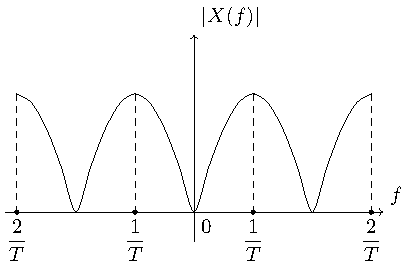
\includegraphics{trasformata-discreta-3.pdf}%
\end{figure}


Data una trasformata di Fourier $X$:
%% grafico
\begin{gather*}
    X(f)=\rect\displaystyle\left(\frac{f}{2f_c}\right)
\end{gather*}
Non può essere la trasformata di una sequenza, poiché deve essere necessariamente periodica. Per cui deve essere espressa come un treno di finestre:
\begin{gather*}
    X(f)=\displaystyle\sum_{k=-\infty}^{\infty}\rect\left(\frac{f-k/T}{2f_c}\right)
\end{gather*}
Per determinare la sequenza associata a questa trasformata si applica l'integrale di antitrasformazione:
\begin{gather*}
    x[n]=T\displaystyle\int_{-1/2T}^{1/2T}\rect\left(\frac{f}{2f_0}\right)e^{2i\pi n fT}\df f=T\int_{-f_c}^{f_c}e^{2i\pi nfT}\df f\\
    \displaystyle\left[T\frac{e^{2i\pi nfT}}{2i\pi fT}\right]^{f_c}_{-f_c}=\frac{2f_cT}{2f_cT}\frac{\sin(2\pi nf_cT)}{\pi n}=2f_cT\sinc(2nf_cT)
\end{gather*}

\subsection{Proprietà del Valor Medio}

Il valor della trasformata di Fourier calcolata in $f=0$ corrisponde al valor medio della sequenza di campioni:
\begin{gather*}
    X(0)=\displaystyle\sum_{k=-\infty}^{+\infty}x[k]
\end{gather*}
Analogamente vale la proprietà duale; il valore del campione in $k=0$, corrisponde al valore medio della trasformata:
\begin{gather*}
    x[0]=\displaystyle\int_{-1/2T}^{1/2T}X(f)df
\end{gather*}

\subsection{Traslazione nel Tempo Discreto ed in Frequenza}

Dato un segnale tempo discreto $x[n]$ e la sua trasformata $X(f)$, si considera un ritardo di $n_0$ campioni e si calcola la sua trasformata rispetto alla trasformata del 
segnale non traslato:
\begin{gather*}
    \mathscr{F}\{x[n-n_0]\}=\displaystyle\sum_{n=-\infty}^{+\infty}x[n-n_0]e^{-2i\pi fnT}=e^{-2i\pi fn_0T}\sum_{m=-\infty}^{+\infty}x[m]e^{-2i\pi mfT}=X(f)e^{-2i\pi fn_0T}
\end{gather*}
Si considera la proprietà duale della traslazione in frequenza, nota una sequenza di campioni $x[n]$ e la sua trasformata di Fourier $X(f)$:
\begin{gather*}
    \mathscr{F}\left\{x[n]e^{2i\pi f_0nT}\right\}=\displaystyle\sum_{k=-\infty}^{+\infty}x[k]e^{2i\pi f_0kT}e^{-2i\pi fkT}=\sum_{k=-\infty}^{+\infty}x[k]e^{-2i\pi (f-f_0)kT}=X(f-f_0)
\end{gather*} 

\subsection{Teorema della Convoluzione}

Data un segnale $y$ convoluzione tra due segnali tempo discreti $x$ e $h$:
\begin{gather*}
    y[n]=x[n]*h[n]=\displaystyle\sum_{k=-\infty}^{+\infty}x[k]h[n-k]
\end{gather*}
Applicando la definizione si ottiene:
\begin{gather*}
    Y(f)=\displaystyle\sum_{n=-\infty}^{+\infty}y[n]e^{-2i\pi nfT}=\displaystyle\sum_{n=-\infty}^{+\infty}\left(\sum_{k=-\infty}^{+\infty}x[k]h[n-k]\right)e^{-2i\pi nfT}
\end{gather*}
Si applica la sostituzione $m=n-k$:
\begin{gather*}
    Y(f)=\displaystyle\sum_{k=-\infty}^{+\infty}\sum_{m=-\infty}^{+\infty}x[k]h[m]e^{-2i\pi kfT}e^{-2i\pi mfT}=\sum_{k=-\infty}^{+\infty}x[k]\left(\sum_{m=-\infty}^{+\infty}h[m]e^{-2i\pi mfT}\right)e^{-2i\pi kfT}\\
    Y(f)=\displaystyle\left(\sum_{k=-\infty}^{+\infty}x[k]e^{-2i\pi kfT}\right)H(f)=X(f)H(f)
\end{gather*}

Dato un segnale $y$ prodotto tra due segnali tempo discreti $x$ e $h$:
\begin{gather*}
    y[n]=x[n]\cdot h[n]
\end{gather*}
Si vuole calcolare la trasformata di Fourier $Y$ nota $X$ e $H$. Si esprime $Y$ tramite la definizione:
\begin{gather*}
    Y(f)=\displaystyle\sum_{n=-\infty}^{+\infty}x[n]h[n]e^{-2i\pi nfT}
\end{gather*}
Si esprime il segnale $x$ come l'antitrasformata del suo spettro in frequenza: 
\begin{gather*}
    Y(f)=\displaystyle\sum_{n=-\infty}^{+\infty}\left(T\int_{-1/2T}^{1/2T}X(\theta)e^{2i\pi n\theta T}\df\theta\right)h[n]e^{-2i\pi nfT}\\
    T\int_{-1/2T}^{1/2T}X(\theta)\left(\sum_{n=-\infty}^{+\infty}h[n]e^{-2i\pi n(f-\theta)T}\right)\df\theta\\
    Y(f)=\displaystyle T\int_{-1/2T}^{1/2T}X(\theta)H(f-\theta)\df\theta
\end{gather*}

\subsubsection{Convoluzione Circolare}

Questa operazione non corrisponde ad una convoluzione tra due segnali periodici $X$ e $H$, poiché la loro convoluzione è data dalla 
convoluzione tra i due segnali $\overline{X}$ e $\overline{H}$:
\begin{gather*}
    {X}(f)*{H}(f)=\displaystyle\int_{-\infty}^{+\infty}\overline{X}(\theta)\overline{H}(f-\theta)\df\theta
\end{gather*}
Questi segnali rappresentano il contenuto informativo in un singolo periodo $1/T$, sono  le basi o repliche che vengono riprodotte ad ogni periodo:
\begin{gather*}
    X(f)=\displaystyle\sum_{n=-\infty}^{+\infty}\overline{X}\left(f-\frac{n}{T}\right)\\
    H(f)=\displaystyle\sum_{k=-\infty}^{+\infty}\overline{H}\left(f-\frac{k}{T}\right)
\end{gather*}
L'operazione ottenuta precedentemente si indica come convoluzione circolare, tra due segnali periodici di periodo uguale $1/T$. Si ottiene come l'integrale 
di convoluzione tra i due segnali su un unico periodo, moltiplicato per l'inverso del periodo:
\begin{gather*}
    X(f) \circledast H(f)=\displaystyle T\int_{-1/2T}^{1/2T}X(\theta)H(f-\theta)\df\theta
\end{gather*}

Si dimostra ora che la convoluzione tra due segnali periodici $X$ e $H$, corrisponde esattamente alla convoluzione circolare tra i due, 
periodicizzata di periodo pari al periodo dei due segnali originali. 


Si considera la convoluzione $\overline{Y}$ tra queste repliche si ottiene come:
\begin{gather*}
    \overline{X}(f)*\overline{H}(f)=\displaystyle\int_{-\infty}^{+\infty}\overline{X}(\theta)\overline{H}(f-\theta)\df\theta=\overline{Y}(f)
\end{gather*}
Si considera la convoluzione circolare $Y$ tra i due segnali $X$ e $H$, esprimendoli come treni di repliche:
\begin{gather*}
    Y(f)=\displaystyle T\int_{-1/2T}^{1/2T}X(\theta)H(f-\theta)\df\theta=T\sum_{n=-\infty}^{+\infty}\sum_{k=-\infty}^{+\infty}\int_{-1/2T}^{1/2T}\overline{X}\left(\theta-\frac{n}{T}\right)\overline{H}\left(f-\theta-\frac{k}{T}\right)\df\theta
\end{gather*}
Si applica la sostituzione $\theta'=\theta-n/T$:
\begin{gather*}
    Y(f)=T\displaystyle\sum_{n=-\infty}^{+\infty}\sum_{k=-\infty}^{+\infty}\int_{-1/2T-n/T}^{1/2T-n/T}\overline{X}(\theta')\overline{H}\left(f-\theta'-\frac{k+n}{T}\right)\df\theta'
\end{gather*}
Il segnale $\overline{X}(\theta')$ assume valori non nulli solo nel periodo centrato in $f=0$, per cui la sommatoria su $n$ fornisce contributi nulli 
per tutti i valori di $n$ eccetto $n=0$
\begin{gather*}
    Y(f)=T\displaystyle\sum_{k=-\infty}^{+\infty}\int_{-1/2T}^{1/2T}\overline{X}(\theta')\overline{H}\left(f-\theta'-\frac{k}{T}\right)\df\theta'
\end{gather*}
Le repliche $\overline{X}$ e $\overline{H}$ sono non nulle solo 
all'interno del periodo base, per cui si possono espandere gli intervalli di integrazione della convoluzione circolare arbitrariamente ottenendo:
\begin{gather*}
    Y(f)=T\displaystyle\sum_{k=-\infty}^{+\infty}\int_{-\infty}^{+\infty}\overline{X}(\theta')\overline{H}\left(f-\theta'-\frac{k}{T}\right)\df\theta'
\end{gather*}
Questa modifica può essere attuata a scopo di calcolo, e non influisce sul risultato finale. Si è quindi ottenuta la convoluzione circolare tra i due segnali $X$ e 
$H$, traslata di un fattore $k/T$:
\begin{gather*}
    Y(f)=T\displaystyle\sum_{k=-\infty}^{+\infty}\overline{Y}\left(f-\frac{k}{T}\right)
\end{gather*}
Si è dimostrato che la convoluzione tra due segnali periodici, di periodo uguale, può essere espressa come la loro convoluzione circolare periodicizzata con lo stesso 
periodo dei due segnali, e moltiplicata per l'inverso del periodo:
\begin{equation}
    X(f)*H(f)=\displaystyle T\sum_{k=-\infty}^{+\infty} X(f) 
    \circledast 
    H(f-k/T)
\end{equation}

\subsection{Teorema di Parseval}

Prima di dimostrare il teorema di Parseval, si determina la trasformata del coniugato di un segnale noto $y$:
\begin{gather*}
    y[n]\to Y(f)
\end{gather*}
Si esprime tramite la definizione:
\begin{gather*}
    \displaystyle\sum_{n=-\infty}^{+\infty}y^*[n]e^{-2i\pi nfT}=\left[\sum_{n=-\infty}^{+\infty}y[n]e^{2i\pi nfT}\right]^*=Y^*(-f)
\end{gather*}

Si considera il duale del teorema della convoluzione:
\begin{gather*}
    \displaystyle\sum_{n=-\infty}^{+\infty}y[n]x[n]e^{-2i\pi nfT}=T\displaystyle\int_{-1/2T}^{1/2T}Y(\theta)X(f-\theta)\df\theta
\end{gather*}
Si pone $f=0$:
\begin{gather*}
    \displaystyle\sum_{n=-\infty}^{+\infty}y[n]x[n]=T\displaystyle\int_{-1/2T}^{1/2T}Y(\theta)X(-\theta)\df\theta
\end{gather*}
Si considera ora $y=y^*$:
\begin{gather*}
    \displaystyle\sum_{n=-\infty}^{+\infty}y^*[n]x[n]=T\displaystyle\int_{-1/2T}^{1/2T}Y^*(-\theta)X(-\theta)\df\theta
\end{gather*}
Si sostituisce ora $x=y$:
\begin{gather*}
    \displaystyle\sum_{n=-\infty}^{+\infty}x^*[n]x[n]=T\displaystyle\int_{-1/2T}^{1/2T}X^*(-\theta)X(-\theta)\df\theta\\
    \displaystyle\sum_{n=-\infty}^{+\infty}|x[n]|^2=T\int_{-1/2T}^{1/2T}|X(\theta)|^2\df\theta
\end{gather*}
Per cui l'energia di un segnale $x$ si può calcolare sia nel tempo discreto che nel dominio della frequenza:
\begin{gather}
    E_x=\displaystyle\sum_{n=-\infty}^{+\infty}|x[n]|^2=T\int_{-1/2T}^{1/2T}|X(f)|^2\df f
\end{gather}

\subsection{Teorema della Correlazione}

Si considera la correlazione tra due segnali tempo discreti $x$ e $y$, e si esprime rispetto alla convoluzione:
\begin{gather*}
    R_{xy}[n]=x[n]\otimes y[n]=\displaystyle\sum_{k=-\infty}^{+\infty}x[n+k]y^*[k]
\end{gather*}
Si vuole calcolare la trasformata del segnale correlazione, tramite la definizione:
\begin{gather*}
    \displaystyle\sum_{n=-\infty}^{+\infty}\sum_{k=-\infty}^{+\infty}x[n+k]y^*[k]e^{-2i\pi nfT}
\end{gather*}
Si applica la sostituzione $m=n+k$:
\begin{gather*}
    \displaystyle\sum_{k=-\infty}^{+\infty}y^*[k]\left(\sum_{m=-\infty}^{+\infty}x[m]e^{-2i\pi mfT}\right)e^{2i\pi kfT}= X(f)\sum_{k=-\infty}^{+\infty}y^*[k]e^{2i\pi kfT}=X(f)Y^*(f)
\end{gather*}
Nel caso in cui $y=x$, allora l'autocorrelazione ha una trasformata di Fourier pari al modulo al quadrato della sua trasformata:
\begin{gather*}
    R_{xx}[n]\to X(f)X^*(f)=|X(f)|^2
\end{gather*}

\subsection{Campionamento}

Un segnale introdotto precedentemente necessario per il campionamento di un segnale è il treno di delta, esprimibile tramite serie di Fourier, poiché periodico:
\begin{gather*}
    \pi(t)=\displaystyle\sum_{n=-\infty}^{+\infty}\delta\left(f-nT\right)=\sum_{k=-\infty}^{+\infty}c_ke^{2i\pi nt/T}
\end{gather*}
I suoi coefficienti si esprimono come:
\begin{gather*}
    c_k=\displaystyle\frac{1}{T}\int_{-T/2}^{T/2}\pi(t)e^{-2i\pi nt/T}\df t=\frac{1}{T}\int_{-T/2}^{T/2}\delta(t)e^{-2i\pi nt/T}\df t=\frac{1}{T}\cancelto{1}{e^{-2i\pi n0/T}}
\end{gather*}
Un treno di delta rappresenta una serie armonica, di ragione $e^{2i\pi t/T}$. La sua trasformata si ottiene come:
\begin{gather*}
    \Pi(f)=\displaystyle\sum_{n=-\infty}^{+\infty}e^{-2i\pi nfT}=\sum_{k=-\infty}^{+\infty}\frac{1}{T}\delta\left(f-\frac{k}{T}\right)
\end{gather*}
La sua trasformata è quindi anch'essa un treno campionatore, con ogni impulso distanziato di un fattore $1/T$ in frequenza. 

Per campionare un segnale si considera un ADC, ``Analog to Digital Converter", un circuito composto da un interruttore che si chiude ad intervalli regolari per misurare il 
valore in entrata: 
\begin{figure}[H]%
    \centering
    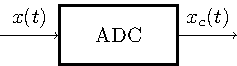
\includegraphics{adc.pdf}%
\end{figure}
Si indica il segnale campionato con $x_c(t)$, mentre il segnale originario con $x(t)$:
\begin{gather*}
    x_c(t)=x(t)\pi(t)=\displaystyle\sum_{n=-\infty}^{+\infty}x(t)\delta\left(t-\frac{n}{T}\right)=\sum_{n=-\infty}^{+\infty}x(nT)\delta\left(t-\frac{n}{T}\right)
\end{gather*}
Il segnale campionato è un segnale tempo continuo, ma si comporta a tutti gli effetti come fosse una sequenza di valori $x[n]$ tempo discreto. 

Si considera ora un campionatore nel dominio della frequenza:
\begin{figure}[H]%
    \centering
    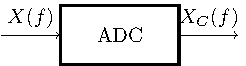
\includegraphics{adc-fourier.pdf}%
\end{figure}

Nel dominio della frequenza il segnale campionato si ottiene come:
\begin{gather*}
    x_c(t)=x(t)\pi(t)=\displaystyle\sum_{n=-\infty}^{+\infty}x(nT)\delta\left(t-nT\right)\\
    X_c(f)=X(f)*\Pi(f)=\displaystyle\sum_{n=-\infty}^{+\infty}x(nT)e^{-2i\pi nfT}\\
    X(f)*\Pi(f)=\displaystyle X(f)*\frac{1}{T}\sum_{n=-\infty}^{+\infty}\delta\left(f-\frac{n}{T}\right)=\frac{1}{T}\sum_{n=-\infty}^{+\infty}X\left(f-\frac{n}{T}\right)
\end{gather*}
Per cui la trasformata del segnale campionato è un segnale periodico nella frequenza, di periodo $1/T$. 
La trasformata di Fourier di una sequenza coincide con la trasformata di Fourier di un segnale campionato. 
Quando le repliche del segnale si sovrappongono, avviene un fenomeno 
noto come ``aliasing", dove a frequenze alte si perdono delle informazioni, poiché si sovrappone con la replica del periodo successivo a basse frequenze. 



Si considera una sequenza $x[n]$ e la sua trasformata:
\begin{gather*}
    x[n]\to X_c(f)=\displaystyle\sum_{n=-\infty}^{+\infty}x[n]e^{-2i\pi nfT}
\end{gather*}
Si può rappresentare la sequenza come un segnale tempo continuo $x$ ad intervalli regolari $T$, chiamato tempo di campionamento:
\begin{gather*}
    x[n]=x(nT)\\
    t=nT\\
    x(t)
\end{gather*}
Per evitare di calcolare la sommatoria si considera la trasformata di questo segnale da cui si è estratta la sequenza: 
\begin{gather*}
    x(t)\to X(f)
\end{gather*}
Per esprimere la trasformata della sequenza si replica questa trasformata ad intervalli $1/T$ in frequenza:
\begin{gather*}
    X_c(f)=\displaystyle\frac{1}{T}\sum_{n=-\infty}^{+\infty}X\left(f-\frac{n}{T}\right)
\end{gather*}

\subsection{Densità Spettrale di Energia}

Per gli integrali tempo continui l'energia di un segnale è definita come:
\begin{gather*}
    E_x=\displaystyle\int_{-\infty}^{+\infty}|x(t)|^2\df x=\int_{-\infty}^{+\infty}|X(f)|^2\df f
\end{gather*}
Mentre per i segnali discreti l'energia viene definita come:
\begin{gather*}
    E_x=\displaystyle\sum_{n=-\infty}^{+\infty}|x[n]|^2
\end{gather*}

La trasformata di Fourier dell'autocorrelazione di un segnale $x$ è pari alla sua energia:
\begin{gather*}
    R_{xx}[n]=\displaystyle\sum_{k=-\infty}^{+\infty}x[n+k]x^*[k]\to X(f)X^*(f)=|X(f)|^2
\end{gather*}
Per cui si può esprimere tramite la sua antitrasformata:
\begin{gather*}
    R_{xx}[n]=T\displaystyle\int_{-1/2T}^{1/2T}|X(f)|^2e^{2i\pi nfT}\df f
\end{gather*}
Per un ritardo nullo $n=0$, l'autocorrelazione corrisponde all'energia di un segnale $x$:
\begin{gather*}
    R_{xx}[n]=T\displaystyle\int_{-1/2T}^{1/2T}|X(f)|^2\df f=E_x
\end{gather*}
Per cui si definisce la densità spettrale di energia l'argomento dell'integrale $|X(f)|^2$, poiché rappresenta la densità dell'energia di un segnale 
ad ogni sua frequenza. 

\subsection{Teorema del Campionamento}

Si considera un sistema di campionamento ADC che prende in ingresso un segnale $x(t)$ tempo continuo, ed ha in uscita un segnale $x_c(t)$, pari ad una 
sommatoria di impulsi estratti dal segnale tempo continuo, ad intervalli regolari del periodo di campionamento $T_c$:
\begin{gather*}
    x_c(t)=x(t)\pi(t)=x(t)\displaystyle\sum_{n=-\infty}^{+\infty}\delta(t-nT_c)=\sum_{n=-\infty}^{+\infty}x(nT)\delta(t-nT)=\sum_{n=-\infty}^{+\infty}x[n]\delta(t-nT)
\end{gather*}
\begin{figure}[H]%
    \centering
    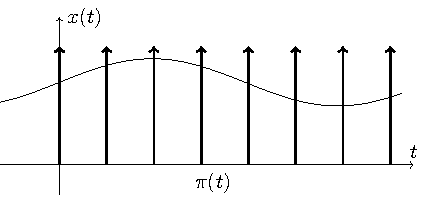
\includegraphics{segnale-campionato.pdf}%
\end{figure}
Nel dominio della frequenza lo spettro del segnale si periodicizza, ovvero corrisponde ad una serie di repliche di periodo $1/T_c$:
\begin{gather*}
    X_c(f)=X(f)*\Pi(f)=\displaystyle\frac{1}{T}\sum_{n=-\infty}^{+\infty}X(f)\delta\left(f-\frac{n}{T}\right)=\frac{1}{T}\sum_{n=-\infty}^{+\infty}X\left(f-\frac{n}{T}\right)=\sum_{n=-\infty}^{+\infty}x[n]e^{-2i\pi nfT}
\end{gather*}

Nel dominio della frequenza si ottiene lo spettro periodicizzato con passo $1/T$. 
\begin{figure}[H]%
    \centering
    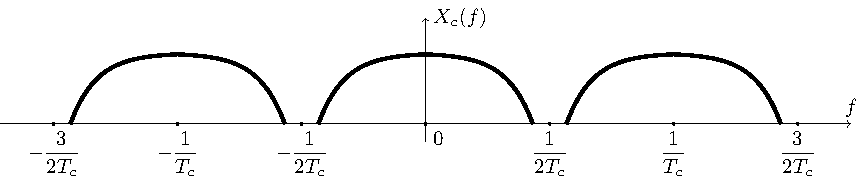
\includegraphics{segnale-campionato-frequenza.pdf}%
\end{figure}

Il teorema del campionamento fornisce una legge per ricostruire una sequenza di campioni in un segnale tempo continuo, con la minima perdita di informazione dal segnale 
originario campionato. Il teorema del campionamento o teorema di Shannon afferma che si può ricostruire perfettamente il segnale originario, soddisfatte una serie di condizioni, 
considerando solamente un'insieme finito di campioni, e non l'intera sequenza. 

Per ricostruire una sequenza di valori si utilizza un filtro DAC ``Digital to Analog Converter". Nel dominio della frequenza, poiché lo spettro del segnale campionato è una 
ripetizione del segnale originario, è sufficiente considerare una singola ripetizione. Per cui la funzione di trasferimento del filtro è una finestra:
\begin{gather*}
    H(f)=T\,\rect(Tf)
\end{gather*}
\begin{figure}[H]%
    \centering
    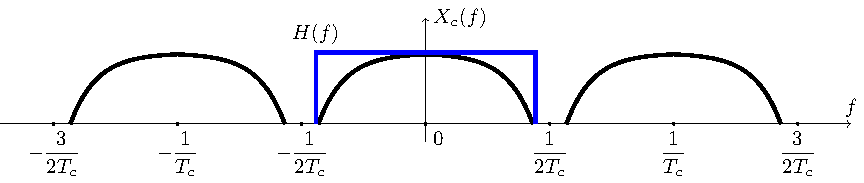
\includegraphics{segnale-replicato-filtro.pdf}%
\end{figure}
In questo modo l'uscita del filtro corrisponde alla trasformata del segnale originario non campionato. 
\begin{figure}[H]%
    \centering
    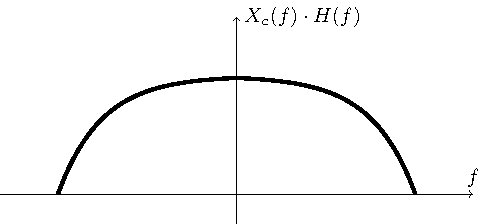
\includegraphics{segnale-replicato-filtrato.pdf}
\end{figure}
Questo filtro è un passa basso ideale. Nel dominio del tempo questo filtro viene descritto da una risposta impulsiva seno cardinale:
\begin{gather*}
    h(t)=\sinc\left(\displaystyle\frac{t}{T}\right)
\end{gather*}
L'uscita nel dominio del tempo è quindi la convoluzione tra la sequenza e la risposta impulsiva del filtro:
\begin{gather*}
    y(t)=\displaystyle\sum_{n=-\infty}^{+\infty}\left[x[n]\delta(t-nT)\right]*\sinc\left(\frac{t}{T}\right)=\sum_{n=-\infty}^{+\infty}x[n]\sinc\left(\frac{t-nT}{T}\right)
\end{gather*}
Per ricostruire un segnale campionato quindi si considerano le somme tra infiniti seni cardinali di ampiezza pari al valore del campione e traslati di un fattore corrispondente. 
\begin{figure}[H]%
    \centering
    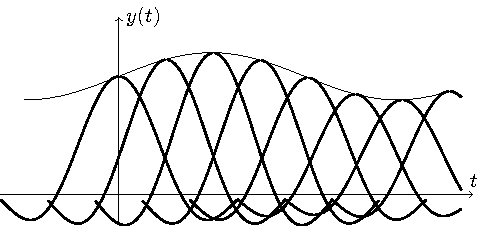
\includegraphics{segnale-ricostruito.pdf}
\end{figure}

Per $t=0$ solo la sinc non traslata da un contributo non nullo, poiché tutte le altre si annullano per valori interi. Ciò è valido per ogni altro valore intero di tempo, dove 
l'unico contributo non nullo coincide con il valore del campione estratto in quel tempo. In questo modo si può ricostruire il segnale originario mantenendo lo stesso contenuto 
informativo, mantenendo solamente una sequenza di valori, campionati dal segnale originario. 


Per ricostruire il segnale bisogna avere un filtro di base abbastanza elevata per contenere il segnale ripetuto. Inoltre è necessario che i segnali ripetuti in frequenza non siano 
sovrapposti tra di loro, altrimenti si verifica il fenomeno noto come aliasing. 
Tutti i segnali reali presentano uno spettro di banda infinito, ma per poter applicare il teorema del campionamento bisogna avere necessariamente un segnale limitato in banda, 
per cui lo spettro di un segnale reale si considera nullo dopo una certa frequenza, chiamata frequenza massima. Per cui prima di digitalizzare il segnale si filtra per 
limitare la banda del segnale. Analogamente bisogna utilizzare un tempo di campionamento abbastanza ridotto per non sovrapporre le repliche del segnale in frequenza. 

La minore frequenza di campionamento possibile affinché non sia presente aliasing corrisponde a due volte la frequenza massima dello spettro del segnale. Questa condizione 
si chiama criterio di Nyquist:
\begin{gather*}
    f_c>2f_{max}\\
    T_c<\displaystyle\frac{1}{2f_{max}}
\end{gather*}
La frequenza massima dipende dal segnale, mentre il tempo di campionamento viene scelto arbitrariamente per soddisfare il criterio di Nyquist. Quando la frequenza di campionamento 
coincide con la frequenza di Nyquist le due repliche coincidono al valore $f=f_{max}$. 

Nel processamento di segnali audio si considera una banda di $4kHz$, per cui nella tecnica PCM ``Pulse Code Modulation" si campiona ad una frequenza di $8kHz$. 
Ad ogni valore della sequenza vengono assegnati $8$ bit, per cui per un segnale audio vengono trasmessi $64k$ bit al secondo. 
Quando non bisogna campionare in tempo reale, si usa una frequenza di campionamento che copra la frequenza massima udibile dall'orecchio umano, pari a $20kHz$, per cui 
i CD Rom adoperano una frequenza di campionamento pari a $44,1kHz$, mentre i DVD campionano fino ad un massimo di $96kHz$. La frequenza di Nyquist quindi dipende dal tipo 
di segnale che si vuole processare, si studieranno in seguito più approfonditamente metodi di processamento di segnali. 

\clearpage

\section{Fenomeni Aleatori}

\subsection{Teoria della Probabilità}


I processi aleatori sono processi il cui valore non è noto a priori. Sono note invece le procedure dell'avvenimento di quell'evento e quindi la probabilità assuma un 
determinato stato. 

I risultati di un fenomeno aleatorio sono univocamente definiti e devono essere completi, si definiscono questo tipo di eventi: eventi elementari. 
L'insieme di tutti i possibili eventi si chiama spazio degli eventi (semplici), in questo spazio sono presenti altri eventi non semplici. 
Si definisce prova l'esecuzione delle procedure definite dall'evento aleatorio, si dice ripetizione una prova ripetuta più volte. Il risultato di una prova può essere favorevole 
o non favorevole. 

Si definisce l'insieme dei possibili risultati di un evento con il simbolo $\mathscr{E}$:
\begin{gather}
    \mathscr{E}:=\{\}
\end{gather}
In uno spazio $\mathbb{R}^n$, e si crea una corrispondenza tra un evento ed un elemento appartenente all'insieme $\mathbb{R}^n$, 
definito da un vettore di dimensione $n$: $\underline{x}=(x_1,\cdots,x_n)\in\mathbb{R}^n$. 
Si definisce il risultato di una prova la variabile $X$, si associa questo valore ad un elemento dello spazio $\mathbb{R}^n$. Questa variabile può essere discreta o continua, 
vettoriale o scalare, sulla base del risultato associato, e le procedure attuate per arrivare a quel risultato. 

Si definisce $\Omega$ l'insieme di tutti i possibili risultati di un evento, chiamato spazio degli eventi semplici. 

Si definisce la funzione probabilità con un approccio frequentistico. Si considera una serie di ripetizioni, e si considera il risultato favorevole delle singole prove $N_E$, diviso per 
tutte le ripetizioni $N$ effettuate, per valori abbastanza grandi di ripetizioni questo valore tende alla frequenza dell'evento $E$:
\begin{gather*}
    f_E=\lim_{N\to\infty}\displaystyle\frac{N_E}{N}
\end{gather*}
Questa definizioni frequentistica si basa sulla legge dei grandi numeri della statistica. Questo valore tende al valore della probabilità dell'evento $E$. 
Questo rapporto per definizione è minore o uguale ad uno, per cui la probabilità che un evento si verifichi deve essere anch'essa minore uguale ad uno:
\begin{gather*}
    P_r\{\mathscr{E}\}\leq1
\end{gather*}
Si dice un evento certo quando la sua probabilità corrisponde ad uno, per cui l'evento $\mathscr{E}$ o coincide con l'insieme degli eventi semplici $\Omega$, oppure lo include. 
Si dice un evento impossibile quando la sua probabilità coincide a zero, ovvero nessuna ripetizione soddisfa questo caso. Per cui per un qualsiasi evento la sua probabilità 
appartiene all'insieme $[0,1]$: $P_r\{\mathscr{E}\}\in[0,1]$. 

Si considera un insieme di eventi disgiunti, se gli eventi sono semplici, necessariamente sono disgiunti. Nota la probabilità dei singoli eventi, la probabilità che avvengano 
tutti gli eventi corrisponde alla somma delle probabilità dei singoli eventi:
\begin{gather*}
    P_r\{\mathscr{E}\}=\displaystyle\sum_{n=1}^{\dim\mathscr{E}}P_r\{{e}_i\}
\end{gather*}
Se gli eventi non sono disgiunti, allora la probabilità che avvenga un evento dipende dagli eventi che sono accaduti precedentemente. 


Si definisce ora la probabilità sulla base di un approccio assiomatico. Si considerano quattro assiomi: 
\begin{itemize}
    \item La probabilità di un evento deve essere maggiore o uguale di zero: $P(A)\geq0$;
    \item La probabilità di un evento certo deve essere uguale ad uno: $P(\Omega)=1$;
    \item La probabilità dell'unione di due eventi disgiunti corrisponde alla somma delle probabilità dei due eventi: $P(A\cup B)=P(A)+P(B)$;
    \item La probabilità dell'unione di eventi disgiunti corrisponde alla somma delle probabilità dei singoli eventi: $P\left(\displaystyle\bigcup_{i=1}^kA_i\right)=\sum_{i=1}^kP(A_i)$;
\end{itemize}

Si associa ad ogni evento un insieme, e si trattano come fossero degli insieme interni allo spazio degli eventi $\Omega$. Si definiscono due eventi $A$ e $B$ disgiunti se la loro 
sovrapposizione produce un insieme vuoto:
\begin{gather*}
    A\cap B=\emptyset
\end{gather*}
Per cui è possibile che avvengano entrambi, poiché la probabilità della loro intersezione non è nulla. 


Si considerano ora una serie di teoremi derivati da questi quattro assiomi: 
Si definisce la probabilità che avvenga un evento di insieme nullo, come impossibile:
\begin{gather*}
    P(\emptyset)=0
\end{gather*}
Si definisce l'evento complementare  $\overline{A}$ all'interno dello spazio degli eventi di $A$ la probabilità che l'evento $A$ non avvenga, e si ottiene come:
\begin{gather*}
    P(\overline{A})=P(\Omega)-P(A)=1-P(A)
\end{gather*}
Se due eventi non sono disgiunti la probabilità che si verifichi uno dei due corrisponde alla somma delle due probabilità tolta la probabilità che avvengano entrambi:
\begin{gather*}
    P(A\cup B)=P(A)+P(B)-P(A\cap B)
\end{gather*}


Si definisce la probabilità condizionata, la probabilità che accada un evento $A$ quando è accaduto $B$:
\begin{gather*}
    P(A|B)=\displaystyle\frac{P(A\cap B)}{P(B)}
\end{gather*} 


Il teorema delle probabilità totali afferma che se una serie di eventi $B_i$ (disgiunti) completa lo spazio degli eventi $\Omega$, allora la probabilità 
che avvenga un evento $A$ si ottiene tramite la seguente espressione: 
\begin{gather*}
    P(A)=\displaystyle\sum_{i=1}^NP(A|B_i)P(B_i)=\sum_{i=1}^N\frac{P(A\cap B_i)}{P(B_i)}P(B_i)=\sum_{i=1}^NP(A\cap B_i)=P(A\cap \Omega)=P(A)
\end{gather*}

Il teorema di Bayes afferma che la probabilità ch avvenga $A$ dato $B$ e la probabilità che avvenga $B$ dato $A$ sono legate tra di loro dalla seguente espressione:
\begin{gather*}
    P(A|B)P(B)=P(B|A)P(A)
\end{gather*}

Con questo teorema si può risolvere il problema di Monty Hall. Si considera la scelta di una delle tre porte $A_1$, $A_2$ e $A_3$, mentre la scelta a posteriori di una delle 
due porte rimanenti $B$. Si considera come prima scelta la porta $A_1$, e si mostra che il premio non si trovi dietro la porta $A_3$. Si calcola la probabilità che il premio 
si trovi dietro la porta $A_1$: 
\begin{gather*}
    P(A_1)=\displaystyle\frac{1}{3}=P(A_2)=P(A_3)\\
    P(A_1|B)=\displaystyle\frac{P(B|A_1)P(A_1)}{P(B)}=\frac{\displaystyle\frac{1}{2}\cdot{\frac{1}{3}}}{P(B)}
\end{gather*}
Sapendo che non può scegliere la porta che contiene il premio, si esprime la probabilità $P(B)$ tramite il teorema delle probabilità totali:
\begin{gather*}
    P(B)=P(B|A_1)P(A_1)+P(B|A_2)P(A_2)+P(B|A_3)P(A_3)=\displaystyle\frac{1}{2}\cdot\frac{1}{3}+1\cdot\frac{1}{3}+0\cdot\frac{1}{3}=\frac{1}{2}\\
    P(A_1|B)=\frac{\displaystyle\frac{1}{2}\cdot{\frac{1}{3}}}{\displaystyle\frac{1}{2}}=\frac{1}{3}
\end{gather*}
Invece la probabilità si trovi dietro alla porta $A_2$:
\begin{gather*}
    P(A_2|B)=\displaystyle\frac{1\cdot\displaystyle\frac{1}{3}}{\displaystyle\frac{1}{2}}=\frac{2}{3}
\end{gather*}
Mentre la probabilità si trovi dietro alla porta $A_3$ è nulla, poiché è stato mostrato non si trovi là:
\begin{gather*}
    P(A_3|B)=0
\end{gather*}

\subsection{Variabili Aleatorie}

Si definisce la variabile aleatoria $X$ una rappresentazione matematica di un problema espresso tramite il linguaggio, mentre si considera una determinazione $x$, un possibile 
valore assunto dalla variabile aleatoria $X$. Si vuole quindi calcolare la probabilità che la variabile aleatoria assuma un certo valore $x$:
\begin{gather*}
    P(X=x)
\end{gather*}
Lo spazio di valori che può assumere la variabile aleatoria può essere discreto o continuo, in base alla descrizione dell'evento. Dato uno spazio degli eventi $\Omega$ ed 
un suo sottoinsieme evento $E$, la probabilità che avvenga l'evento appartiene al codominio $[0,1]$, mentre l'insieme delle determinazioni della variabile aleatoria 
associata appartiene all'insieme $\mathbb{R}^n$:
\begin{gather*}
    P: E\to[0,1]\\
    X:E\to\mathbb{R}^n
\end{gather*}

Si considera un resistore che può assumere tre valori di resistenza $R_1=40\,\Omega$, $R_2=50\,\Omega$ e $R_3=\,\Omega$. La probabilità assuma questi tre valori è:
\begin{gather*}
    P(R=40\,\Omega)=0.1\\
    P(R=50\,\Omega)=0.6\\
    P(R=60\,\Omega)=0.3
\end{gather*}
Si considera la probabilità che il resistore assuma un valore minore o uguale di un certo valore $x$, questa funzione viene definita funzione di distribuzione cumulativa $D(x)$:
\begin{gather}
    P(R\leq x)=D_R(x)
\end{gather}
\begin{figure}[H]%
    \centering
    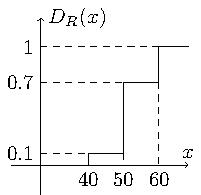
\includegraphics{distribuzione-cumulativa.pdf}%
\end{figure}

La funzione di distribuzione cumulativa deve essere monotona crescente, può essere formata da gradini, ma deve essere sempre crescente. In generale per una variabile 
aleatoria $X$, all'aumentare della variabile $x$, le probabilità si sommano, per cui il valore tende asintoticamente ad un valore $1$, mentre tende ad un valore nullo 
per $x\to-\infty$:
\begin{gather*}
    \lim_{x\to-\infty}D_X(x)=0\\
    \lim_{x\to+\infty}D_X(x)=1
\end{gather*}
Per una variabile aleatoria discreta si può esprimere come la somma delle probabilità che la variabile assuma il valore della realizzazione $x_i$, moltiplicate per un gradino 
che parte dal valore $x_i$:
\begin{gather}
    D_X(x)=\displaystyle\sum_{i=-\infty}^{+\infty}P_iu(x-x_i)
\end{gather}
Dove:
\begin{gather*}
    x\in\{x_1,\cdots,x_n\}\\
    P_i=P(x=x_i)
\end{gather*}

Si considera la variabile aleatoria tempo di attesa $t$, uniformemente distribuita. Assume valori compresi nell'intervallo $[0,T]$, rappresenta il tempo di attesa prima 
che avvenga un evento. La sua funzione di distribuzione di probabilità assuma una forma:
\begin{figure}[H]%
    \centering
    \includegraphics{distribuzione-probabilità.pdf}%
\end{figure}

La pendenza della curva si ottiene tramite $1/T$. 



La funzione densità di probabilità $P_X$, della variabile aleatoria $X$ calcolata in $x$, si esprime come la derivata della funzione di distribuzione di probabilità:
\begin{equation}
    P_X(x)=\displaystyle\frac{\df D_X(x)}{\df x}
\end{equation}
La funzione di distribuzione cumulativa è quindi una primitiva della funzione densità di probabilità:
\begin{equation}
    D_X(x)=\displaystyle\int_{-\infty}^{x}P_X(\xi)\df\xi
\end{equation}
Per una variabile aleatoria discreta, la funzione densità di probabilità rappresenta una serie di impulsi, centrati nel valore $x_i$, di ampiezza la probabilità $P_i$:
\begin{equation}
    P_X(x)=\displaystyle\sum_{i=-\infty}^{+\infty}P_i\delta(x-x_i)
\end{equation}

La funzione densità di probabilità della variabile aleatoria tempo di attesa rappresenta una finestra di ampiezza $1/T$ di base $T$ e centrata in $T/2$:
\begin{figure}[H]%
    \centering
    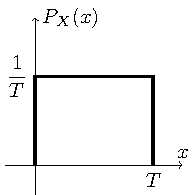
\includegraphics{densità-probabilità.pdf}%
\end{figure}

Si può calcolare la probabilità la variabile aleatoria assumi un valore compreso in un intervallo $[a,b]$, si può esprimere come una differenza di distribuzioni di 
probabilità, oppure come l'integrale della densità di probabilità sull'intervallo considerato:
\begin{equation}
    P(a\leq x\leq b)=D_X(b)-D_X(a)
\end{equation}
\begin{gather*}
    D_X(b)-D_X(a)=\displaystyle\int_{-\infty}^bP_X(x)\df x-\int_{-\infty}^aP_X(x)\df x\\
    \int_{-\infty}^bP_X(x)\df x+\int^{-\infty}_aP_X(x)\df x=\int_a^bP_X(x)\df x
\end{gather*}
\begin{equation}
    P(a\leq x\leq b)=\displaystyle\int_a^bP_X(x)\df x
\end{equation}
Per la variabile aleatoria tempo di attesa, la probabilità assuma un valore nell'intervallo $[a,b]$ si ottiene come:
\begin{gather*}
    P(a\leq t\leq b)=\displaystyle\int_a^b\frac{1}{T}\df t=\frac{b-a}{T}
\end{gather*}
La densità di probabilità deve essere normalizzata, per cui il suo integrale sull'intervallo dove è definita la variabile aleatoria deve tendere al valore $1$:
\begin{equation}
    \displaystyle\int_{\mathbb{R}^n}P_X(x)\df x=1
\end{equation}

\subsection{Statistiche Notevoli}

La statistica più nota è quella gaussiana, in questa statistica, la funzione densità di probabilità della variabile aleatoria $x$ assume la seguente forma:
\begin{equation}
    P_X(x)=\displaystyle e^{-\left(\frac{x-\mu_x}{\sqrt{2}\sigma_x}\right)^2}\frac{1}{\sqrt{2\pi}\sigma_x}
\end{equation}
%% grafico 
Si chiama $\sigma_x$ deviazione standard, mentre il suo quadrato si definisce varianza. Il valore dove è centrata la gaussiana $\mu_x$ si chiama valor medio. 
Questa funzione deve rispettare la condizione di chiusura. 
L'integrale su tutti le possibili determinazioni della densità di probabilità di $x$ corrisponde all'integrale di Gauss:
\begin{gather*}
    \displaystyle\int_{-\infty}^{+\infty}P_x(x)\df x=\int_{-\infty}^{+\infty}e^{-\frac{(x-\mu_x)^2}{2\sigma_x^2}}\frac{1}{\sqrt{2\pi}\sigma_x}\df x\\
    t=\displaystyle\frac{x-\mu_x}{\sqrt{2}\sigma_x}\\
    \displaystyle\int_{_\infty}^{+\infty}e^{-t^2}\frac{\sqrt{2}{\sigma_x}}{\sqrt{2}\sigma_x}\frac{1}{\sqrt{pi}}{\df x}=\frac{\sqrt{\pi}}{\sqrt{\pi}}=1
\end{gather*}
La sua distribuzione di probabilità si ottiene come:
\begin{gather*}
    D_X(x)=\displaystyle\int_{-\infty}^xP_X(\overline{x})\df\overline{x}
\end{gather*}
%% grafico
Un altra funzione molto utilizzata è la Laplaciana. La probabilità della variabile aleatoria $x$ è quindi della forma:
\begin{equation}
    P_X(x)=\lambda e^{-\lambda x}u(x)
\end{equation}
%% grafico 

Si verifica la condizione di normalizzazione:
\begin{gather*}
    \displaystyle\int_{-\infty}^{+\infty}P_X(x)\df x=\int_{-\infty}^{+\infty}\lambda e^{-\lambda x}u(x)\df x=\int_0^{+\infty}xe^{-\lambda x}\df x=-e^{-\lambda x}\Bigg|_0^{+\infty}=1
\end{gather*}
La sua distribuzione di probabilità si ottiene come:
\begin{gather*}
    D_X(x)=\displaystyle\int_{-\infty}^xP_X(\overline{x})\df\overline{x}=u(x)\int_0^x\lambda e^{-\lambda\overline{x}}\df\overline{x}=-e^{-\lambda\overline{x}}\Bigg|_0^xu(x)=\left(1-e^{-\lambda x}\right)u(x)
\end{gather*}
%% grafico

\subsection{Variabili Aleatorie Dipendenti}

Sia data una variabile aleatoria di cui sia nota la statistica $X$, e una variabile aleatoria $Y$, di cui non si conosce la statistica, espressa rispetto ad $X$ tramite la 
seguente espressione:
\begin{gather*}
    Y=aX+b
\end{gather*}
%% grafico 

Si calcola la funzione di distribuzione cumulativa di $Y$:
\begin{gather*}
    D_Y(y)=P(Y\leq y)
\end{gather*}
Poiché è una relazione lineare, questa relazione si può esprimere rispetto alla variabile $X$:
\begin{gather*}
    y=f(x)=ax+b\\
    x=g(y)=\displaystyle\frac{y-b}{a}\\
    P(Y\leq y)=P\left(X\leq\displaystyle\frac{y-b}{a}\right)\\
    D_Y(y)=D_X\left(\displaystyle\frac{y-b}{a}\right)=D_X(g(y))
\end{gather*}
\begin{equation}
    D_Y(y)=D_X(g(y))
\end{equation}

La densità di probabilità si ottiene derivando la distribuzione cumulativa:
\begin{gather*}
    P_Y(y)=\displaystyle\frac{\df}{\df y}D_Y(y)\\
    \frac{\df}{\df y}D_X(g(y))=\frac{\df}{\df x}D_X(g(y))\frac{\df x}{\df y}\\ % chain-rule
    P_X(g(y))\frac{\df}{\df y}g(y)
\end{gather*}
Per cui si può esprimere la densità di probabilità della variabile $Y$ rispetto alla densità nota della variabile $X$:
\begin{equation*}
    P_Y(y)=P_X(g(y))g'(y)
\end{equation*}

Se la curva che lega le due variabili è decrescente allora la distribuzione della variabile $Y$ può essere espressa rispetto alla probabilità che la variabile $X$ sia 
maggiore del valore per cui la determinazione di $Y$ è minore del valore $y$: 
%% grafico
\begin{gather*}
    D_Y(y)=P(Y\leq y)=P\left(\displaystyle X>\frac{y-b}{a}\right)\\
    1-P\left(X\leq\frac{y-b}{a}\right)=1-D_X\left(\frac{y-b}{a}\right)
\end{gather*}
Derivando questa relazione si ottiene:
\begin{gather*}
    P_Y(y)=\displaystyle\frac{\df}{\df y}D_Y(y)\\
    -\displaystyle\frac{\df}{\df x}D_X\left(\frac{y-b}{a}\right)=-P_X(g(y))g'(y)
\end{gather*}
Per cui bisogna tenere conto della pendenza della curva che lega le due variabili aleatorie:
\begin{equation}
    P_Y(y)=P_X(g(y))\left|g'(y)\right|
\end{equation}


In caso la relazione $y=f(x)$ tra le due variabili non sia invertibile, si divide il dominio in $N$ tratti dove la funzione che lega le due variabile è monotona crescente o 
decrescente in modo da poter esprimere la loro relazione inversa $x=g_i(y)$. In questo modo si può applicare la formula dimostrata precedentemente su ogni 
sotto-insieme del dominio per ottenere la densità di probabilità della variabile $Y$:
\begin{gather*}
    P_Y(y)=\displaystyle\sum_{i=1}^NP_{Y,i}(y)=\sum_{i=1}^NP_X(g_i(y))|g_i'(y)|
\end{gather*} 

\subsection{Parametri Statistici}
\label{sec:parametri-statistici}

I parametri statistici di una variabile aleatoria $X$ sono dei valori associati alla variabile, non sono funzioni, ma possono essere parametrici. 

Si definisce il valore medio o valore attesto di una variabile aleatoria discreta $X$, capace di assumere $N$ realizzazioni:
\begin{gather*}
    x\in\left\{x_1,\cdots,x_N\right\}
\end{gather*}
Se vengono effettuate $M$ ripetizioni, viene definito il valore medio $\mu_x$ come il numero di volte $n_i$ che si verifica una delle realizzazioni $x_i$ moltiplicata per 
il valore della realizzazione, per ognuna delle $N$ realizzazioni, diviso per il numero totale di ripetizioni:
\begin{equation}
    \mu_x=\displaystyle\frac{\displaystyle\sum_{i=1}^Nn_ix_i}{M}=\sum_{i=1}^Nx_iP_i
\end{equation}

Per una variabile aleatoria continua, il valore medio è definito come:
\begin{equation}
    \mu_x=\displaystyle\int_{-\infty}^{+\infty}xP_X(x)\df x
\end{equation}
Viene chiamato anche come ``expectation'', e può essere espresso come:
\begin{equation}
    \mu_x=E[x]
\end{equation}


Inserendo nell'integrale per una variabile aleatoria continua la densità di probabilità di una variabile discreta, si ottiene la definizione per una variabile aleatoria discreta:
\begin{gather*}
    P_X(x)=\displaystyle\sum_{i=1}^NP_i\delta(x-x_i)\\
    \mu_x=\displaystyle\int_{-\infty}^{+\infty}x\sum_{i=1}^NP_i\delta(x-x_i)\df x=\sum_{i=1}^NP_i\int_{-\infty}^{+\infty}x\delta(x-x_i)\df x=\sum_{i=1}^Nx_iP_i
\end{gather*}


Il valore atteso di una variabile aleatoria uniforme, distribuita sull'intervallo $[a,b]$, si ottiene come:
\begin{gather*}
    \mu_x=\displaystyle\int_{-\infty}^{+\infty}xP_X(x)\df x=\int_{a}^b\frac{1}{b-a}\df x=\frac{b^2-a^2}{2(b-a)}=\frac{b-a}{2}
\end{gather*}


Si calcolare ora il valore medio di una variabile aleatoria di statistica gaussiana:
\begin{gather*}
    P_X(x)=\displaystyle\frac{1}{\sqrt{2\pi}\sigma_x}e^{-\frac{(x-\mu_x)^2}{\sigma_x^2}}\\
    \mu_x=\displaystyle\int_{-\infty}^{+\infty}xP_X(x)\df x=\int_{-\infty}^{+\infty}\frac{x}{\sqrt{2\pi}\sigma_x}e^{-\frac{(x-\mu_x)^2}{\sigma_x^2}}\df x
\end{gather*}
Si applica un cambio di variabile $t=(x-\mu_x)/(\sqrt{2}\sigma_x)$:
\begin{gather*}
    \mu_x=\displaystyle\int_{-\infty}^{+\infty}\frac{\sqrt{2}\sigma_xt+\mu_x}{\sqrt{2\pi}\sigma_x}e^{-t^2}\sqrt{2}\sigma_x\df t=\cancelto{0}{\int_{-\infty}^{+\infty}\sqrt{2}\sigma_xte^{-t^2}}\df t+\frac{\mu_x}{\sqrt{\pi}}\int_{-\infty}^{+\infty}e^{-t^2}\df t=\mu_x\cancelto{1}{\frac{\sqrt{\pi}}{\sqrt{\pi}}}
\end{gather*}
Si è dimostrato che il fattore di traslazione di una gaussiana $\mu_x$ corrisponde al suo valore medio. 


Si calcola il valore medio di una statistica esponenziale:
\begin{gather*}
    P_X(x)=\lambda e^{-\lambda x}u(x)\\
    \mu-x=\displaystyle\int_{-\infty}^{+\infty}xP(x)\df x=\lambda\int_{0}^{+\infty}xe^{-\lambda x}\df x=\cancelto{0}{\left[xe^{-\lambda x}\right]_0^{+\infty}}+\int_0^{+\infty}e^{-\lambda x}\df x\\
    \mu_x=\displaystyle\cancelto{0}{\left[-xe^{-\lambda x}\right]_0^{+\infty}}+\left[-\frac{e^{-\lambda x}}{\lambda}\right]_0^{+\infty}=\frac{1}{\lambda}
\end{gather*}


Si definisce il valore atteso quadratico o il momento del secondo ordine $\mu_x^{(2)}$ come:
\begin{equation}
    \mu_x^{(2)}=\displaystyle\int_{-\infty}^{+\infty}x^2P_X(x)\df x=E[x^2]
\end{equation}

Si definisce il momento centrato del secondo ordine $E[(x-\mu_x)^2]$ o varianza:
\begin{equation}
    \sigma_x^2=\displaystyle\int_{-\infty}^{+\infty}(x-\mu_x)^2P_X(x)\df x=E[(x-\mu_x)^2]
\end{equation}
La varianza fornisce informazioni sull'estensione della distribuzione intorno al valore medio. 


Si definisce la deviazione standard $E[x-\mu_x]$:
\begin{equation}
    \sigma_x=\displaystyle\int_{-\infty}^{+\infty}(x-\mu_x)P_X(x)\df x=E[x-\mu_x]
\end{equation}


Si calcola il momento centrato del secondo ordine tramite la definizione:
\begin{gather*}
    E\left[(x-\mu_x)^2\right]=\displaystyle\int_{-\infty}^{+\infty}(x-\mu_x)^2P_X(x)\df x=\sigma_x^2\\
    \int_{-\infty}^{+\infty}x^2P_X(x)\df x-\int_{-\infty}^{+\infty}x\mu_xP_X(x)\df x+\mu_x^2\int_{-\infty}^{+\infty}P_X(x)\df x\\
    \mu_x^{(2)}+\mu_x^2\int_{-\infty}^{+\infty}P_X(x)\df x-2\mu_x\int_{-\infty}^{+\infty}xP_X(x)\df x
\end{gather*}
Il primo integrale corrisponde al momento del secondo ordine, il secondo integrale assume valore unitario poiché la densità di probabilità è normalizzata e l'ultimo 
integrale corrisponde al valore medio:
\begin{gather*}
    \sigma_x^2=\mu_x^{(2)}+\mu_x^2-2\mu_x\mu_x=\mu_x^{(2)}-\mu_x^2
\end{gather*}

Data una statistica esponenziale, si calcola la sua deviazione standard tramite la definizione:
\begin{gather*}
    \mu_x^{(2)}=\displaystyle\int_{-\infty}^{+\infty}x^2\lambda e^{-\lambda x}u(x)\df x=\cancelto{0}{\left[-x^2e^{-\lambda x}\right]_0^{+\infty}}+2\int_{0}^{+\infty}xe^{-\lambda x}\df x\\
    \cancelto{0}{\left[-2\displaystyle\frac{e^{-\lambda x}}{\lambda}\right]_0^{+\infty}}+2\int_{0}^{+\infty}\frac{e^{-\lambda x}}{\lambda}\df x=\left[-\frac{2}{\lambda^2}\right]^{+\infty}_0=\frac{2}{\lambda^2}
\end{gather*}
Mentre la sua varianza si ottiene come:
\begin{gather*}
    \sigma_x^2=\mu_x^{(2)}-\mu_x^2=\displaystyle\frac{2}{\lambda^2}-\frac{1}{\lambda^2}=\frac{1}{\lambda}
\end{gather*}


Data una statistica gaussiana, si calcola la sua varianza:
\begin{gather*}
    E[(x-\mu_x)^2]=\displaystyle\int_{-\infty}^{+\infty}(x-\mu_x)^2e^{-\frac{(x-\mu_x)^2}{2\sigma_x^2}}\frac{\df x}{\sqrt{2\pi}\sigma_x}\\
    t=\displaystyle\frac{x-\mu_x}{\sqrt{2}\sigma_x}\\
    \displaystyle\int_{-\infty}^{+\infty}t^22\sigma_x^2e^{-t^2}\frac{\df t}{\sqrt{\pi}}=\cancelto{0}{\left[\frac{1}{\sqrt{\pi}}2\sigma_x^2\left(\frac{-te^{-t^2}}{2}\right)\right]}+\frac{2\sigma_x^2}{\sqrt{\pi}}\int_{-\infty}^{+\infty}\frac{e^{-t^2}}{2}\df t=\sigma_x^2
\end{gather*}


Data una statistica uniforma, si calcola il momento del secondo ordine:
\begin{gather*}
    \mu_x^{(2)}=\displaystyle\int_{-\infty}^{+\infty}x^2P_X(x)\df x=\int_a^bx^2\frac{\df x}{b-a}=\frac{1}{3}\frac{b^3-a^3}{b-a}=\frac{b^2+ab+a^2}{3}
\end{gather*}

Si calcola ora la sua varianza:
\begin{gather*}
    \sigma_x^2=\mu_x^{(2)}-\mu_x^2=\displaystyle\frac{b^2+ab+a^2}{3}-\frac{(b+a)^2}{4}=\frac{(b-a)^2}{12}
\end{gather*}



Si definisce la funzione caratteristica come:
\begin{equation}
    E\left[e^{-2i\pi fx}\right]=\displaystyle\int_{-\infty}^{+\infty}e^{-2i\pi fx}p_X(x)\df x=\mathscr{P}_X(f)
\end{equation}
Corrisponde alla trasformata di Fourier della densità di probabilità. 

La derivata della funzione caratteristica rispetto alla frequenza si ottiene il seguente termine:
\begin{gather*}
    \displaystyle\frac{\df}{\df f}\mathscr{P}_X(f)=-2i\pi\int_{-\infty}^{+\infty}xP_X(x)e^{-2i\pi fx}\df x\\
    \displaystyle-\frac{1}{2i\pi}\frac{\df}{\df f}\mathscr{P}_X(f)\bigg|_{f=0}=\int_{-\infty}^{+\infty}xP_X(x)\df x=\mu_x
\end{gather*}

Si calcola la funzione caratteristica di una statistica uniforme, gaussiana ed esponenziale:
\begin{gather*}
    P_X(x)=\displaystyle\frac{1}{b-a}\rect\left(\frac{x-(b-a)/2}{b-a}\right)\\
    \mathscr{P}_X(f)=\displaystyle\sinc\left[(b-a)f\right]e^{-i\pi f(b-a)}
\end{gather*}
La trasformata di una gaussiana è una gaussiana, come è stato precedentemente calcolato: 
\begin{gather*}
    P_X(x)=\frac{1}{\sqrt{2\pi}\sigma_x}e^{-\frac{(x-\mu_x)^2}{2\sigma_x^2}}\\
    \mathscr{P}_X(f)=e^{-\pi^2\sigma_x^2f^2}e^{-2i\pi f\mu_x}
\end{gather*}
Analogamente è stata già calcolata la trasformata di una funzione esponenziale: 
\begin{gather*}
    P_X(x)=\lambda e^{-\lambda x}u(x)\\
    \mathscr{P}_X(f)=\displaystyle\frac{\lambda}{\lambda+2i\pi f}
\end{gather*}


Si considerano i parametri precedentemente definiti:
\begin{gather*}
    E[x]=\mu_x\\
    E[x^2]=\mu_x^{(2)}\\
    E[(x-\mu_x)^2]=\sigma_x^2\\
    E\left[e^{-2i\pi fx}\right]=\mathscr{P}_X(f)
\end{gather*}
Tramite la funzione ``expectation", e questi altri parametri appena definiti, è possibile esprimere le variabili aleatorie. Date due variabili aleatorie legate dalla 
relazione $f(x)=y$, si può calcolare il valore atteso della variabile $y$ come:
\begin{gather*}
    E[y]=\displaystyle\int_{-\infty}^{*\infty}yP_Y(y)\df y=\int_{-\infty}^{+\infty}f(x)P_X(x)\df x=E[f(x)]
\end{gather*}

Gode della proprietà di linearità:
\begin{gather*}
    E[af(x)+bg(x)]=\displaystyle\int_{-\infty}^{+\infty}(af(x)+bg(x))P_X(x)\df x\\
    a\int_{-\infty}^{+\infty}f(x)P_X(x)\df x+b\int_{-\infty}^{+\infty}g(x)P_X(x)\df x=aE[f(x)]+bE[g(x)]
\end{gather*}

\subsection{Variabile Aleatoria Bidimensionale}

Si considera una variabile aleatoria definita da due variabili $X$ e $Y$. Si calcola la sua distribuzione di probabilità:
\begin{gather*}
    D_{X,Y}(x,y)=P(X\leq x,Y\leq y)
\end{gather*}
Si definisce la densità di probabilità congiunta, la derivata seconda di questa distribuzione di probabilità:
\begin{gather*}
    \displaystyle\frac{d^2}{\df x\df y}D_{X,Y}(x,y)=P_{X,Y}(x,y)
\end{gather*}
Se la variabile aleatoria è discreta si esprime questa densità congiunta come una doppia sommatoria:
\begin{gather*}
    P_{X,Y}(x,y)=\displaystyle\sum_{i=1}^N\sum_{j=1}^M\delta(x-x_i)\delta(y-y_j)
\end{gather*}
Deve soddisfare la condizione di normalizzazione sull'intero piano:
\begin{gather*}
    \iint_{\mathbb{R}^2}P_{X,Y}(x,y)\df x\df y=1
\end{gather*}
Altrimenti ci si riferisce alle densità di probabilità marginali, integrando la probabilità congiunta rispetto a solo una variabile, rimuovendo la dipendenza della funzione 
dalla variabile di integrazione. Si dice che si ``satura" una delle due variabili aleatorie, poiché non si considera più la sua statistica. Per una variabile 
bidimensionale si hanno quindi due probabilità marginali:
\begin{gather*}
    \displaystyle\int_{-\infty}^{+\infty}P_{X,Y}(x,y)\df y=P_X(x)\\
    \displaystyle\int_{-\infty}^{+\infty}P_{X,Y}(x,y)\df x=P_Y(y)
\end{gather*}
Se e solo se le dua variabili sono indipendenti tra di loro, allora la probabilità congiunta fattorizza e rappresenta il prodotto tra le due densità di probabilità marginali:
\begin{gather*}
    P_{X,Y}(x,y)=P_X(x)P_Y(y)
\end{gather*}

Per determinare il valore atteso si considera:
\begin{gather*}
    E[f(x,y)]=\displaystyle\iint_{\mathbb{R}^2}f(x,y)P_{X,Y}(x,y)\df x\df y
\end{gather*}
Si quindi estendono tutti gli integrali calcolati precedentemente sull'intero piano, per calcolare i parametri statistici di una variabile aleatoria bidimensionale. 

Si definisce il momento misto di ordine $1,1$ o correlazione:
\begin{gather*}
    E[xy]=\displaystyle\iint_{\mathbb{R}^2}xyP_{X,Y}(x,y)\df x\df y=\mu_{x,y}^{1,1}
\end{gather*}
Questo parametro quantifica se i due segnali aleatori sono correlati tra di loro. Se i due segnali sono indipendenti tra di loro, allora il momento misto di ordine $1,1$ si 
può calcolare come:
\begin{gather*}
    E[xy]=\displaystyle\iint_{\mathbb{R}^2}xyP_{X,Y}(x,y)\df x\df y=\iint_{\mathbb{R}^2}(xP_X(x))(yP_Y(y))\df x\df y
\end{gather*}
Poiché le variabili di integrazione sono indipendenti è possibile separare gli integrali:
\begin{gather*}
    \displaystyle\int_{-\infty}^{+\infty}xP_X(x)\df x\cdot\int_{-\infty}^{+\infty}yP_Y(y)\df y=\mu_x\mu_y
\end{gather*}


Si definisce la covarianza $\sigma_{x,y}$ di una variabile aleatoria bidimensionale come:
\begin{gather*}
    \sigma_{x,y}=E[(x-\mu_x)\cdot(y-\mu_y)]
\end{gather*}
Se $X=Y$, ovvero se le due variabili aleatorie indipendenti sono la stessa variabile, allora la covarianza sarebbe la varianza $\sigma_x^2$. 
Si esprime la covarianza tramite la definizione integrale:
\begin{gather*}
    \sigma_{x,y}=\iint_{\mathbb{R}^2}(x-\mu_x)(y-\mu_y)P_{X,Y}(x,x)\df x\df y\\
    \displaystyle\iint_{\mathbb{R}^2}xyP_{X,Y}(x,y)\df x\df y-\mu_x\int_{-\infty}^{+\infty}y\left(\int_{-\infty}^{+\infty}P_{X,Y}(x,y)\df x\right)\df y\\
    -\displaystyle\mu_y\int_{-\infty}^{+\infty}x\left(\int_{-\infty}^{+\infty}P_{X,Y}(x,y)\df y\right)\df x+\mu_x\mu_y\cancelto{1}{\iint_{\mathbb{R}^2}P_{X,Y}(x,y)\df x\df y}\\
    \displaystyle\iint_{\mathbb{R}^2}xyP_{X,Y}(x,y)\df x\df y-\mu_x\int_{-\infty}^{+\infty}yP_Y(y)\df y-\mu_y\int_{-\infty}^{+\infty}xP_X(x)\df x+\mu_x\mu_y\\
    \mu_{x,y}^{1,1}-\mu_x\mu_y-\mu_x\mu_y+\mu_x\mu_y
\end{gather*}
\begin{equation}
    \sigma_{x,y}=\mu_{x,y}^{1,1}-\mu_x\mu_y
\end{equation}

Tramite la covarianza si studia il grado di correlazione tra due variabili aleatorie per identificare se sono legate. 
L'indice di correlazione $\rho_{x,y}$ è definito come:
\begin{equation}
    \rho_{x,y}=\displaystyle\frac{\sigma_{x,y}}{\sqrt{\sigma_x^2\sigma_y^2}}=\frac{\sigma_{x,y}}{\sigma_x\sigma_y}
\end{equation}
Questo valore è compreso nell'intervallo $[0,1]$, se la covarianza è uguale a $0$ le due variabili sono in-correlate, mentre se è pari ad $1$, le due variabili sono 
correlate e probabilmente dipendenti dallo stesso fenomeno. 


Verrà trattato un unico caso di variabile aleatoria bidimensionale dipendente:

Si considera una variabile $Z$ definita come la combinazione lineare di due variabili aleatorie $X$ e $Y$ indipendenti. 
\begin{gather*}
    Z=X+Y
\end{gather*}
Si vuole determinare la sua densità di probabilità. 
Poiché sono indipendenti si può esprimere la densità di probabilità congiunta rispetto alle densità di probabilità marginali:
\begin{gather*}
    P_{X,Y}(x,y)=P_X(x)P_Y(y)
\end{gather*}

Si calcola il valore atteso della funzione caratteristica di $Z$:
\begin{gather*}
    \mathscr{P}_z(f)=\displaystyle\int_{-\infty}^{+\infty}ze^{-2i\pi fz}\df z\\
    z=x+y\\
    E[e^{-2i\pi fz}]=E[e^{-2i\pi f(x+y)}]\\
    E[e^{-2i\pi f(x+y)}]\displaystyle=\iint_{\mathbb{R}^2}e^{-2i\pi f(x+y)}P_{X,Y}(x,y)\df x\df y\\
    \displaystyle\int_{-\infty}^{+\infty}e^{-2i\pi fx}P_X(x)\df x\int_{-\infty}^{+\infty}e^{-2i\pi fy}P_Y(y)\df y=\mathscr{P}_x(f)\mathscr{P}_y(f)\\
    \mathscr{P}_z(f)=E[e^{-2i\pi fz}]=E[e^{-2i\pi f(x+y)}]=\mathscr{P}_x(f)\mathscr{P}_y(f)
\end{gather*}
\begin{equation}
    \mathscr{P}_z(f)=\mathscr{P}_x(f)\cdot\mathscr{P}_y(f)
\end{equation}

Poiché rappresentano la trasformata della densità di probabilità, ritornando nel dominio della variabile aleatoria, l'operazione rappresenta una convoluzione 
tra le due densità di probabilità $P_X$ e $P_Y$:
\begin{equation}
    P_Z(z)=P_X(x)*P_Y(y)
\end{equation}


Si calcola il valore atteso di $Z$, utilizzando la proprietà di linearità della funzione ``expectation'':
\begin{gather*}
    \mu_z=E[z]=E[x+y]=E[x]+E[y]=\mu_x+\mu_y
\end{gather*}
\begin{equation}
    \mu_z=\mu_x+\mu_y
\end{equation}

Si calcola il momento del secondo ordine di $Z$:
\begin{gather*}
    \mu_z^{(2)}=E[z^2]=E[(x+y)^2]=E[x^2]+2E[xy]+E[y^2]=\mu_x^{(2)}+2\mu_{x,y}^{(1,1)}+\mu_y^{(2)}
\end{gather*}
Poiché le due variabili sono indipendenti si può esprimere come:
\begin{gather}
    \mu_z^{(2)}=\mu_x^{(2)}+2\mu_x\mu_y+\mu_y^{(2)}
\end{gather}

Si calcola la varianza della variabile aleatoria $Z$:
\begin{gather*}
    \sigma_z^2=\mu_z^{(2)}-\mu_z^2=\mu_x^{(2)}+2\mu_x\mu_y+\mu_y^{(2)}-(\mu_x+\mu_y)^2=\mu_x^{(2)}-\mu_x^2+\mu_y^{(2)}-\mu_y^2=\sigma_x^2+\sigma_y^2
\end{gather*}
\begin{equation}
    \sigma_z^2=\sigma_x^2+\sigma_y^2
\end{equation}

\subsection{Processi Aleatori}

Dato un sistema composto da $N$ o infinite sorgenti della stessa tipologia, indipendenti tra di loro, ognuno associato ad un segnale nel tempo univoco. L'insieme di questi 
segnali viene chiamato processo aleatorio, poiché il segnale che varia nel tempo è del tipo aleatorio o stocastico o non deterministico. 

Si vogliono introdurre delle variabili e caratteristiche per individuare il processo e studiarne i parametri stocastici per analizzare i segnali. 
Si sceglie un istante di tempo $t_1$ e si misura per ogni sorgente il segnale prodotto $x_i(t_1)$, che rappresentano tutte le possibili realizzazioni della variabile 
aleatoria discreta o continua $X_1$:
\begin{gather*}
    X_1:=\left\{x_1(t_1),\cdots,x_N(t_1)\right\}
\end{gather*}

Questa variabile aleatoria puù essere analizzata per produrre i valori dei suoi parametri statistici, come è stato analizzato precedente \ref{sec:parametri-statistici}. 
Introducendo una nuova variabile $X_2$ misurando il valore in un istante di tempo diverso $t_2$, si possono analizzare le proprietà ed i parametri bidimensionali 
delle due variabili. 

In generale dato un istante di tempo $t_j$ ed un processo aleatoria, si definisce una gerarchia del primo ordine, la variabile aleatoria, discreta o continua, che può 
assumere come possibili realizzazioni tutti i possibili valori dei segnali del processo aleatorio nell'istante di tempo $t_j$:
\begin{equation}
    X_j=\left\{x_1(t_j),x_2(t_j),\cdots\right\}
\end{equation}
Quindi dato un processo aleatorio e fissati gli istanti di tempo possono essere estratte, possono essere estratte un numero corrispondente di variabili aleatorie. 
In caso si studi la funzione di correlazione o la covarianza tra due di gerarchie del primo ordine, si tratta di gerarchie del secondo ordine. 


Sia dato un processo aleatorio definito dal segnale $x(t)=A\cos(2\pi t/T)$, dove l'ampiezza del segnale è uniformemente distribuita sull'intervallo $[0,1]$. 
Se viene scelto come istante di tempo $t_1$ il periodo, per estrarre i valori del processo, si ottiene una variabile aleatoria con una distribuzione pari alla densità di probabilità 
dell'ampiezza:
\begin{gather*}
    P_A(A)=\rect\displaystyle\left(A-\frac{1}{2}\right)\\
    x(t_1=T)=A\cos(2\pi)=A\\
    X_1=A\\
    P_{X_1}(x_1)=\displaystyle\rect\left(x_1-\frac{1}{2}\right)
\end{gather*}
Invece scegliendo un tempo $t_2=T/2$:
\begin{gather*}
    x(t_2=T/2)=-A\\
    X_2=-A=-X_1\\
    P_{X_2}(x_2)=-\displaystyle\rect\left(x_1-\frac{1}{2}\right)=-P_{X_1}(x_2)
\end{gather*}
Per $t_3=T/4$ si ha:
\begin{gather*}
    x(t_3=T/4)=0\\
    P_{X_3}(x_3)=\delta(x_3)
\end{gather*}

Si vuole calcolare il valore medio di questo processo aleatorio, definito dalla variabile aleatoria $X=x(t)$
\begin{gather*}
    E[X]=\displaystyle\int_{-\infty}^{+\infty}x(t)P_x(x)\df x
\end{gather*}
Poiché l'ampiezza rende il processo stocastico, si integra rispetto a quest'ultima:
\begin{gather*}
    \displaystyle\int_{-\infty}^{+\infty}A\cos\left(\frac{2\pi t}{T}\right)P_A(A)dA=\cos\left(\frac{2\pi t}{T}\right)\int_0^1AdA=\frac{1}{2}\cos\left(\frac{2\pi t}{T}\right)
\end{gather*}
Si calcola ora il valore quadratico medio:
\begin{gather*}
    \mu_x^{(2)}=E[x(t)^2]\displaystyle\int_{-\infty}^{+\infty}A^2\cos^2\left(\frac{2\pi t}{T}\right)P_A(A)dA=\cos\left(\frac{2\pi t}{T}\right)\int_0^1A^2dA=\frac{1}{3}\cos^2\left(\frac{2\pi t}{T}\right)
\end{gather*}


Noto il valore medio ed il valore quadratico medio, si può calcolare la varianza del processo aleatorio:
\begin{gather*}
    \sigma_x^2=E[(x(t)-\mu_x)^2]=\mu_x^{(2)}-\mu_x^2=\displaystyle\frac{1}{3}\cos^2\left(\frac{2\pi t}{T}\right)-\frac{1}{4}\cos^2\left(\frac{2\pi t}{T}\right)=frac{1}{12}\cos^2\left(\frac{2\pi t}{T}\right)
\end{gather*}

Si calcolano le gerarchie del secondo ordine tra due variabile aleatorie estratte negli istanti di tempo $t_1$ e $t_2$. Partendo dalla correlazione si ottiene:
\begin{gather*}
    E[x(t_1),x(t_2)]=\displaystyle\iint_{\mathbb{R}^2}x(t_1)x(t_2)P_{X_1,X_2}(x_1,t_2,x_2,t_2)\df x_1\df x_2\\    
    \displaystyle\int_{-\infty}^{+\infty}A\cos\left(\frac{2\pi t_1}{T}\right)A\cos\left(\frac{2\pi t_2}{T}\right)\rect\displaystyle\left(A-\frac{1}{2}\right)\df A=\cos\left(\frac{2\pi t_1}{T}\right)\cos\left(\frac{2\pi t_2}{T}\right)\int_0^1A^2\df A\\
    R_X(t_1,t_2)=\displaystyle\frac{1}{3}\cos\left(\frac{2\pi t_1}{T}\right)\cos\left(\frac{2\pi t_2}{T}\right)
\end{gather*}
Per questo processo la correlazione dipende sia da $t_1$ che $t_2$ separatamente. 

\subsubsection{Processo Armonico}

Il processo aleatorio precedentemente descritto  rappresenta un oscillatore, ma nella realtà non quando si crea un oscillatore la frequenza è accurata, ma la fase iniziale rappresenta un fattore casuale, o 
variabile stocastico: 
\begin{equation*}
    x(t)=\displaystyle\cos\left(\frac{2\pi t}{T}+\varphi\right)
\end{equation*}
Questo processo prende il nome di processo armonico. 
Si considera la fase $\varphi$ uniformemente distribuita tra $0$ e $2\pi$:
\begin{gather*}
    P_{\varphi}(\varphi)=\displaystyle\frac{1}{2\pi}\rect\left(\frac{\varphi-\pi}{2\pi}\right)
\end{gather*}

In generale è difficile effettuare un aggancio in fase, dato che la fase iniziale dipende da parametri che spesso non vengono controllati. 
Si calcolano le statistiche di questo processo aleatorio:
\begin{gather*}
    \mu_{x}=E[x(t)]=\displaystyle\int_{-\infty}^{+\infty}\cos\left(\frac{2\pi t}{T}+\varphi\right)\frac{1}{2\pi}\rect\left(\frac{\varphi-\pi}{2\pi}\right)\df\varphi=\frac{1}{2\pi}\int_0^{2\pi}\cos\left(\frac{2\pi t}{T}+\varphi\right)\df\varphi\\
    \frac{1}{2\pi}\sin\left(\frac{2\pi t}{T}+2\pi\right)-\frac{1}{2\pi}\sin\left(\frac{2\pi t}{T}\right)=0
\end{gather*}
Si calcola il valore quadratico medio, utilizzando le formula di duplicazione del coseno inversa, per esprimere il coseno quadro:
\begin{gather*}
    \mu_{x}^{(2)}=E[x(t)^2]=\displaystyle\int_{-\infty}^{+\infty}\cos^2\left(\frac{2\pi t}{T}+\varphi\right)\frac{1}{2\pi}\rect\left(\frac{\varphi-\pi}{2\pi}\right)\df\varphi\\
    \frac{1}{2\pi}\int_0^{2\pi}\left[\frac{1}{2}+\frac{1}{2}\cos\left(\frac{4\pi t}{T}+2\varphi\right)\right]\df\varphi\\
    \frac{1}{4\pi}\int_0^{2\pi}\df\varphi+\frac{1}{4\pi}\cancelto{0}{\int_0^{2\pi}\cos\left(\frac{4\pi t}{T}+2\varphi\right)\df\varphi}=\frac{2\pi}{4}-0=\frac{1}{2}
\end{gather*}
La sua varianza è quindi:
\begin{gather*}
    \sigma_x^2=\mu_x^{(2)}-\mu_x^2=\displaystyle\frac{1}{2}-0=\frac{1}{2}
\end{gather*}

Le statistiche così calcolate non dipendono dal tempo. 

Si calcolano ora le gerarchie del secondo ordine tra due variabili aleatorie estratte in tempi $t_1$ e $t_2$:
\begin{gather*}
    X_1=x(t_1)=\displaystyle\cos\left(\frac{2\pi t_1}{T}+\varphi\right)\\
    X_2=x(t_2)=\displaystyle\cos\left(\frac{2\pi t_2}{T}+\varphi\right)\\
    E[x_1x_2]=\displaystyle\iint_{\mathbb{R}^2}x_1x_2P_{X_1,X_2}(x_1,,t_1,x_2,t_2)\df x_1\df x_2\\
    \displaystyle\iint_{\mathbb{R}^2}\cos\left(\frac{2\pi t_1}{T}+\varphi\right)\cos\left(\frac{2\pi t_2}{T}+\varphi\right)\frac{1}{2\pi}\rect\left(\frac{\varphi-\pi}{2\pi}\right)\df\varphi\\
    \displaystyle\frac{1}{4\pi}\cancelto{0}{\int_{0}^{2\pi}\cos\left[\frac{2\pi(t_1+t_2)}{T}+2\varphi\right]\df\varphi}+\frac{1}{4\pi}\int_{0}^{2\pi}\cos\left[\frac{2\pi(t_1-t_2)}{T}\right]\df\varphi\\
    \mu_{x_1,x_2}=\displaystyle\frac{1}{2}\cos\left[\frac{2\pi(t_1-t_2)}{T}\right]\cancelto{1}{\int_0^{2\pi}\frac{\df\varphi}{2\pi}}
\end{gather*}
Questa correlazione tra due variabili aleatorie estratte dallo stesso processo, prende il nome di autocorrelazione


La covarianza tra due variabili aleatorie estratte dallo stesso processo:
\begin{gather*}
    C_X(t_1,t_2)=R_X(t_1,t_2)-\mu_{x_1}(t_1)\mu_{x_2}(t_2)
\end{gather*}
Per un processo armonico, il valore medio è sempre nullo per ogni variabile aleatoria estratta, per cui la covarianza è uguale alla correlazione tra le due variabili 
estratte in $t_1$ e $t_2$:
\begin{gather*}
    C_X(t_1,t_2)=R_X(t_1,t_2)=\displaystyle\frac{1}{2}\cos\left[\frac{2\pi(t_1-t_2)}{T}\right]
\end{gather*} 

Inoltre si esprime l'indice di correlazione $\rho_{X}(t_1,t_2)$ come:
\begin{gather*}
    \rho_X(t_1,t_2)=\displaystyle\frac{C_X(t_1,t_2)}{\sqrt{\sigma_x^2(t_1)\sigma_x^2(t_2)}}
\end{gather*}

\subsubsection{Processi Stazionari}

Un processo stazionario per definizione presenta gerarchie del primo ordine indipendenti dal tempo, e gerarchie del secondo ordine dipendenti solo dalla differenza tra due 
istanti di tempo. 

Per questioni di semplicità si analizzano solamente processi reali, per cui nell'integrale di correlazione non sarà necessario considerare l'operazione di coniugato. In 
un processo stazionario dipende solo dalla differenza $\tau$ tra due istanti di tempo dove sono estratte le variabili aleatorie, come la covarianza:
\begin{gather*}
    R_X(\tau)=E[x(t+\tau)x^*(t)]=E[x(t+\tau)x(t)]=x(t)\otimes x(t)
\end{gather*}
Valgono le proprietà trattate precedentemente sull'operazione di correlazione \ref{sec:correlazione}, senza considerare il coniugato:
\begin{gather*}
    R_X(\tau)=R_x(-\tau)
\end{gather*} 
La correlazione è massima per $\tau=0$:
\begin{gather*}
    R_X(0)=E[x(t)x(t)]=E[x(t)^2]=P_X
\end{gather*}
La correlazione nell'origine coincide con la potenza del segnale. 


Le stesse proprietà che valgono per le variabili aleatorie generiche, valgono per variabili aleatorie estratte da due processi aleatori stazionari e indipendenti:
\begin{gather*}
    z(t)=x(t)+y(t)
    \mu_z=E[z(t)]=E[x(t)+y(t)]=\mu_x+\mu_y
\end{gather*}
Si calcola la correlazione tra queste due:
\begin{gather*}
    R_Z(\tau)=E[z(t+\tau)z(t)]=\displaystyle\int_{-\infty}^{+\infty}zP_Z(z)\df z\\
    E[z(t+\tau)z(t)]=E[(x(t+\tau)+y(t+\tau))(x(t)+y(t))]\\
    E[x(t+\tau)x(t)]+E[x(t+\tau)y(t)]+E[y(t+\tau)x(t)]+E[y(t+\tau)y(t)]\\
    R_X(\tau)+E[x(t+\tau)]E[y(t)]+E[x(t)]E[y(t+\tau)]+R_Y(\tau)\\
    R_Z(\tau)==R_X(\tau)+R_Y(\tau)+2\mu_x\mu_y
\end{gather*}
La densità spettrale di potenza si ottiene del processo aleatorio dipendente $z$ si ottiene come:
\begin{gather*}
    G_Z(f)=\int{-\infty}^{+\infty}\left(R_X(\tau)+R_Y(\tau)+2\mu_x\mu_y\right)e^{-2i\pi f\tau}\df \tau=G_X(f)+G_Y(f)+2\mu_x\mu_y\delta(f)
\end{gather*}

\subsubsection{Processo Ergotico}

Questa caratteristica è indipendente dalla stazionarietà, ma viene trattata come se fosse associata ad essa. 
Questi processi vengono descritti da un unica realizzazione. Ovvero le caratteristiche del processo dipendono da una sola realizzazione, traslata nel tempo. 

Per questi processi le medie temporali coincidono con le medie di insieme. Ovvero le statistiche calcolate tramite la funzione ``expectation'', possono essere 
calcolate sull'integrale rispetto al tempo del segnale:
\begin{gather*}
    E[x(t)]=\displaystyle\int_{-\infty}^{+\infty}x(t)P_X(x)\df x=\int_{-\infty}^{+\infty}x(t)\df t\\
    \widetilde{x(t)}=\overline{x(t)}^t
\end{gather*}
formalmente l'integrale rispetto al tempo si esprime tramite un limite, come per il calcolo della potenza di un segnale:
\begin{gather*}
    E[x(t)]=\lim_{\Delta T\to+\infty}\displaystyle\frac{1}{\Delta T}\int_{-\Delta T/2}^{\Delta T/2}x(t)\df t\\
    P_X=E[x^2(t)]=\lim_{\Delta T\to+\infty}\displaystyle\frac{1}{\Delta T}\int_{-\Delta T/2}^{\Delta T/2}x^2(t)\df t
\end{gather*}


Un processo armonico è un processo stazionario ed ergotico, per cui si calcola il suo valore medio rispetto al tempo:
\begin{gather*}
    \mu_x=\overline{x(t)}^t=\lim_{\Delta T\to+\infty}\displaystyle\frac{1}{\Delta T}\int_{-\Delta T/2}^{\Delta T/2}\cos\left(\frac{2\pi t}{T}+\varphi\right)\df t=0
\end{gather*}
Poiché il coseno è una funzione limitata nell'intervallo $[0,1]$, questo limite tende a zero. 


Nota la funzione di correlazione $R_X(\tau)$, la sua trasformata si indica come lo spettro densità di potenza $G_X(f)$:
\begin{gather*}
    G_X(f)=\displaystyle\int_{-\infty}^{+\infty}R_X(\tau)e^{-2i\pi f\tau}\df\tau=\mathscr{F}\{R_X(\tau)\}
\end{gather*}
Si chiama densità di potenza, poiché se viene integrata su tutte le frequenze restituisce la potenza $P_X$ del segnale:
\begin{gather*}
    R_X(0)=\displaystyle\int_{-\infty}^{+\infty}G_X(f)df=P_X
\end{gather*}

Per un processo armonico, il suo spettro densità di potenza si ottiene come:
\begin{gather*}
    R_X(\tau)=\displaystyle\frac{1}{2}\cos\left(\frac{2\pi t}{T}\right)\to G_X(f)=\displaystyle\frac{1}{4}\delta\left(f-\frac{1}{T}\right)+\frac{1}{4}\delta\left(f+\frac{1}{T}\right)
\end{gather*}

\subsubsection{Rumore}
Il rumore viene classificato come un processo aleatorio, dipendente dal tempo, e nella maggior parte dei casi si indica come rumore additivo gaussiano bianco 
``Additive White Gaussian Noise'' (AVGN) $n(t)$. 
Si dice additivo, poiché quando si analizza un segnale, si somma il rumore se è presente nel sistema:
\begin{gather*}
    x(t)+n(t)
\end{gather*} 

Questo rumore ha una statistica gaussiana. Il rumore ha valor medio nullo $\mu_n=0$. 
Per calcolare la varianza si sfrutta la densità spettrale di potenza, poiché questo processo è bianco, la densità spettrale di potenza è costante. 
Si dice bianco, poiché la luce bianca ha uno spettro di frequenze costante, si mantiene il termine per ogni tipo di segnale avente una densità spettrale di potenza 
costante. 

Se fosse veramente costante, allora la potenza di questo processo sarebbe infinita:
\begin{gather*}
    G_X(f)=k\\
    P_X=\displaystyle\int_{-\infty}^{+\infty}kdf=+\infty
\end{gather*}

Per cui si dice che è costante in banda, ovvero nell'intervallo di frequenze $[-\omega,\omega]$ dove si sta lavorando:
\begin{gather*}
    G_X(f)=\displaystyle K\rect\left(\frac{f}{2\omega}\right)
\end{gather*}
La potenza di questa densità spettrale in banda è quindi:
\begin{gather*}
    P_X=\displaystyle\int_{-\infty}^{+\infty}G_X(f)\df f=\int_{-\omega}^{+\omega}K\df f=2\omega K
\end{gather*}


La sua funzione di autocorrelazione è un impulso, per cui due campioni di ritardo $\tau$ estratti da questo processo non sono mai correlati, eccetto quando coincidono
$t_1=t_2\to \tau=0$:
\begin{gather*}
    \mathscr{F}^{-1}\{G_X(f)\}=k\delta(\tau)=R_X(\tau)
\end{gather*}
Se la densità spettrale è in banda, allora la funzione di autocorrelazione è un seno cardinale:
\begin{gather*}
    G_X(f)=\displaystyle K\rect\left(\frac{f}{2\omega}\right)\\
    R_X(\tau)=2\omega K\sinc(2\omega\tau)
\end{gather*}

Il rumore più studiato è il rumore termico, o di Johnson-Nyquist. Questo rumore dipende dalla temperatura, e la sua varianza vale:
\begin{gather*}
    \sigma_x^2=\displaystyle\frac{2\pi^2k_\mathrm{B}T^2R_\mathrm{eq}}{3\hbar}
\end{gather*}

Quando viene misurata la tensione di un circuito, si misura questo rumore che aumenta la sua varianza intorno al valor medio all'aumento della temperatura. 
Poiché il valore medio è nullo, la varianza coincide con il momento del secondo ordine, e quindi, al valore della potenza del segnale:
\begin{gather*}
    \sigma_x^2=\mu_x^{(2)}-\mu_x^2=\mu_x^{(2)}=E[x^2(t)]=P_X
\end{gather*}

\subsubsection{Transito Attraverso un Sistema}

Nell'ambito dei processi aleatori i sistemi possono essere definiti con memoria o senza memoria. Un sistema si dice senza memoria, se la sua uscita per ogni istante di 
tempo $t$ dipende interamente dall'entrata in quell'istante di tempo, mentre si dice con memoria, se l'uscita dipende anche dallo stato interno del sistema. 

I filtri sono sistemi con memoria, poiché l'uscita corrisponde alla convoluzione tra l'ingresso e la risposta impulsi del sistema. 

Dato un sistema senza memoria $y(t)=ax(t)+b$, e la statistica dell'entrata $X$, si determinano la statistiche dell'uscita $Y$:
\begin{gather*}
    \mu_y=E[y(t)]=E[ax(t)+b]=a[x(t)]+b=a\mu_x+b\\
    \mu_y^{(2)}=E[y^2(t)]=a^2E[x^2(t)]+2abE[x(t)]+b^2=a^2\mu_x^{(2)}+2ab\mu_x+b^2\\
    P_Y=a^2P_X+2ab\mu_x+b\\
    \sigma_y^2=\mu_y^{(2)}-\mu_y^2=a^2\mu_x^{(2)}+2ab\mu_x+b^2-(a\mu_x+b)^2=a^2\mu_x^{(2)}-a^2\mu_x^2=a^2\sigma_x^2\\
    R_Y(\tau)=E[y(t+\tau)y(\tau)]=E[(ax(t+\tau)+b)(ax(t)+b)]\\
    a^2E[x(t+\tau)x(t)]+abE[x(t+\tau)]+abE[x(t)]+b^2=a^2R_X(\tau)+2ab\mu_x+b^2\\
    P_Y=R_Y(0)=a^2R_X(0)+2ab\mu_x+b^2=a^2P_X+2ab\mu_x+b^2\\
    C_Y(\tau)=R_Y(\tau)-\mu_y^2=a^2R_X(\tau)+2ab\mu_x+b^2-a^2\mu_x^2-2ab\mu_x-b^2=a^2R_X(\tau)-a^2\mu_x^2=a^2C_Y(\tau)\\
    \rho_Y(\tau)=\displaystyle\frac{C_Y(\tau)}{\sqrt{\sigma_y^2}}=\frac{a^2C_X(\tau)}{\sqrt{a^2\sigma_x^2}}=\frac{C_X(\tau)}{\sqrt{\sigma_x^2}}
\end{gather*}


Dato un filtro $y(t)=x(t)*h(t)$, e nota la statistica dell'entrata $X$, si determinano le statistiche dell'uscita $Y$:
\begin{gather*}
    \mu_y=E[y(t)]=E[x(t)*h(t)]=E[x(t)]*h(t)=\displaystyle\mu_x\int_{-\infty}^{+\infty}h(t')\df t'=\mu_xH(0)
\end{gather*}
Dato che la risposta impulsiva integrata su tutti i reali coincide con la funzione di trasferimento del filtro, a frequenze nulle:
\begin{gather*}
    \displaystyle\int_{-\infty}^{+\infty}h(t)e^{-2i\pi ft}\df t=H(f)\\
    H(0)=\displaystyle\int_{-\infty}^{+\infty}h(t)\df t
\end{gather*}
Prima di calcolare la funzione di autocorrelazione del processo $y(t)$, bisogna determinare la correlazione tra i processi $x(t)$ e $y(t)$:
\begin{gather*}
    R_{yx}(\tau)=E[y(t+\tau)x^*(t)]=E[y(t+\tau)x(t)]=E\left[\displaystyle\int_{-\infty}^{+\infty}h(t')x(t+\tau-t')\df t'x(t)\right]\\
    \displaystyle\int_{-\infty}^{+\infty}h(t')E[x(t+\tau-t')x(t)]\df t'=\displaystyle\int_{-\infty}^{+\infty}h(t')R_X(\tau-t')\df t'=h(\tau)*R_X(\tau)
\end{gather*}
La funzione di autocorrelazione di $y(t)$ è quindi:
\begin{gather*}
    R_Y(\tau)=E[y(t+\tau)y(t)]=E\left[y(t+\tau)\displaystyle\int_{-\infty}^{+\infty}h(t')x(t-t')\df t'\right]=\int_{-\infty}^{+\infty}h(t')E[y(t+\tau)x(t-t')]\df t'\\
    \displaystyle\int_{-\infty}^{+\infty}h(t)R_{yx}(\tau+t')\df t'=h(\tau)\otimes R_{yx}(\tau)=h(-\tau)*R_{yx}(\tau)=h(-\tau)*h(t)*R_X(\tau)
\end{gather*}
La densità spettrale dell'uscita si ottiene trasformando quest'ultima relazione:
\begin{gather*}
    G_Y(f)=H^*(f)H(f)G_X(f)=|H(f)|^2G_X(f)
\end{gather*}


\end{document}